\documentclass[english,10pt,a4paper,oneside]{book}
\usepackage[english]{babel}

% PAGE GEOMETRY
\usepackage{geometry}
\geometry{margin=4cm}

% FONTS
% with lining figures for math roman; load before other text specs:
% \usepackage{eulervm}
\usepackage{amssymb,amsmath}
\usepackage{ifxetex}
\ifxetex
  \usepackage{microtype}
  \usepackage{mathspec} % only with xelatex; before fontspec
  \usepackage{fontspec} % only with xelatex
  % \defaultfontfeatures{Ligatures=Common}
  \setmainfont[Ligatures=TeX]{Minion Pro}
  \setsansfont[Ligatures=TeX,Scale=MatchLowercase]{Myriad Pro}
  \setmonofont[Scale=.85]{Ubuntu Mono}
  % custom ampersand
  \newcommand{\amper}{{\fontspec[Scale=.95]{Hoefler Text}\selectfont\itshape\&}}
\else
  \usepackage[activate={true,nocompatibility},final,tracking=true,kerning=true,spacing=true,factor=1100,stretch=10,shrink=10]{microtype}
  \usepackage[T1]{fontenc}
  \usepackage[utf8]{inputenc}
  \DeclareUnicodeCharacter{2212}{-}
\fi

% TYPOGRAPHY SETTINGS
% disable protrusion for tt fonts
\UseMicrotypeSet[protrusion]{basicmath}
% remove excessive space after full-stop
\frenchspacing

% % CHAPTER HEADINGS
% \usepackage{sectsty} % don't work with 'quotchap'
% \chapterfont{\usefont{T1}{qhv}{b}{n}\selectfont\huge}
% qotation ahead of chapters and fancy chapter heading
\usepackage{quotchap}
\renewcommand*{\sectfont}{\sffamily\bfseries\Huge\selectfont}

% SECTION, SUBSECTION, ETC. TITLES
\usepackage[compact]{titlesec}
% \titleformat{\chapter} % don't work with 'quotchap'
%   {\normalfont\Huge\sffamily\bfseries}
%   {\thechapter}
%   {1em}
%   {}
\titleformat{\section}
  {\normalfont\LARGE\sffamily\bfseries}
  {\thesection}
  {1em}
  {}
\titleformat{\subsection}
  {\normalfont\Large\sffamily\bfseries}
  {\thesubsection}
  {1em}
  {}
\titleformat{\subsubsection}
  {\normalfont\large\sffamily\bfseries\slshape}
  {\thesubsubsection}
  {1em}
  {}
% \titlespacing*{<command>}{<left>}{<before-sep>}{<after-sep>}
\titlespacing*{\section}
  {0pt}
  {1.2ex plus 1ex minus .2ex}
  {0.5ex plus .1ex minus .1ex}
\titlespacing*{\subsection}
  {0pt}
  {1.2ex plus 1ex minus .2ex}
  {0.5ex plus .1ex minus .1ex}
\titlespacing*{\subsubsection}
  {0pt}
  {1.2ex plus 1ex minus .2ex}
  {0.5ex plus .1ex minus .1ex}

% FIGURE AND TABLE CAPTIONS
\usepackage{floatrow}
\floatsetup[figure]{capposition=bottom}
\floatsetup[table]{capposition=top}

% QUOTATIONS AND QUOTATION MARKS
\usepackage[autostyle]{csquotes} % works with babel
% use upquote if available, for straight quotes in verbatim environments
\usepackage{upquote}{}

% HYPERLINKS
\usepackage{hyperref}
\hypersetup{
    colorlinks=true,
    linkcolor=blue,
    filecolor=magenta,
    urlcolor=cyan,
}
\urlstyle{same}
% avoid problems with \sout in headers with hyperref
\usepackage[normalem]{ulem}
\pdfstringdefDisableCommands{\renewcommand{\sout}{}}

% FOOTNOTES
\usepackage{fancyvrb}
\VerbatimFootnotes % allows verbatim text in footnotes
% Make links footnotes instead of hotlinks
\renewcommand{\href}[2]{#2\footnote{\url{#1}}}
% Use protect on footnotes to avoid problems with footnotes in titles
\let\rmarkdownfootnote\footnote%
\def\footnote{\protect\rmarkdownfootnote}

% BIBLIOGRAPHY
\usepackage{natbib}

% TABLES
\usepackage{longtable,booktabs,tabularx,ragged2e,dcolumn,multirow,multicol}
\setlength\heavyrulewidth{0.1em}
\setlength\lightrulewidth{0.0625em}

% SI UNITS
\usepackage{siunitx}
    \sisetup{%
        detect-mode,
        group-digits            = false,
        input-symbols           = ( ) [ ] - + < > * §,
        table-align-text-post   = false,
        round-mode              = places,
        round-precision         = 3
        }

% GRAPHICS SETTINGS
\usepackage{graphicx,grffile}
\makeatletter
\def\maxwidth{\ifdim\Gin@nat@width>\linewidth\linewidth\else\Gin@nat@width\fi}
\def\maxheight{\ifdim\Gin@nat@height>\textheight\textheight\else\Gin@nat@height\fi}
\makeatother
% Scale images if necessary, so that they will not overflow the page
% margins by default, and it is still possible to overwrite the defaults
% using explicit options in \includegraphics[width, height, ...]{}
\setkeys{Gin}{width=\maxwidth,height=\maxheight,keepaspectratio}

% LINESPACING
% \usepackage{setspace}
% \setstretch{1.5}

% NO INDENTATION WITH A SPACE BETWEEN PARAGRAPHS
\usepackage{parskip}
\setlength{\parindent}{0pt}
\setlength{\parskip}{6pt plus 2pt minus 1pt}
% prevent overfull lines
\setlength{\emergencystretch}{3em}
\providecommand{\tightlist}{%
  \setlength{\itemsep}{0pt}\setlength{\parskip}{0pt}}

% THE NEXT LINES OF CODE SPECIFY SOME YAML ENTRIES %
%%%%%%%%%%%%%%%%%%%%%%%%%%%%%%%%%%%%%%%%%%%%%%%%%%%%
% switch yes/no in YAML header

% ENABLES LISTING OF CODE (echo = TRUE)
% listings: yes/no
\usepackage{color}
\usepackage{fancyvrb}
\newcommand{\VerbBar}{|}
\newcommand{\VERB}{\Verb[commandchars=\\\{\}]}
\DefineVerbatimEnvironment{Highlighting}{Verbatim}{commandchars=\\\{\}}
% Add ',fontsize=\small' for more characters per line
\usepackage{framed}
\definecolor{shadecolor}{RGB}{248,248,248}
\newenvironment{Shaded}{\begin{snugshade}}{\end{snugshade}}
\newcommand{\AlertTok}[1]{\textcolor[rgb]{0.94,0.16,0.16}{#1}}
\newcommand{\AnnotationTok}[1]{\textcolor[rgb]{0.56,0.35,0.01}{\textbf{\textit{#1}}}}
\newcommand{\AttributeTok}[1]{\textcolor[rgb]{0.77,0.63,0.00}{#1}}
\newcommand{\BaseNTok}[1]{\textcolor[rgb]{0.00,0.00,0.81}{#1}}
\newcommand{\BuiltInTok}[1]{#1}
\newcommand{\CharTok}[1]{\textcolor[rgb]{0.31,0.60,0.02}{#1}}
\newcommand{\CommentTok}[1]{\textcolor[rgb]{0.56,0.35,0.01}{\textit{#1}}}
\newcommand{\CommentVarTok}[1]{\textcolor[rgb]{0.56,0.35,0.01}{\textbf{\textit{#1}}}}
\newcommand{\ConstantTok}[1]{\textcolor[rgb]{0.00,0.00,0.00}{#1}}
\newcommand{\ControlFlowTok}[1]{\textcolor[rgb]{0.13,0.29,0.53}{\textbf{#1}}}
\newcommand{\DataTypeTok}[1]{\textcolor[rgb]{0.13,0.29,0.53}{#1}}
\newcommand{\DecValTok}[1]{\textcolor[rgb]{0.00,0.00,0.81}{#1}}
\newcommand{\DocumentationTok}[1]{\textcolor[rgb]{0.56,0.35,0.01}{\textbf{\textit{#1}}}}
\newcommand{\ErrorTok}[1]{\textcolor[rgb]{0.64,0.00,0.00}{\textbf{#1}}}
\newcommand{\ExtensionTok}[1]{#1}
\newcommand{\FloatTok}[1]{\textcolor[rgb]{0.00,0.00,0.81}{#1}}
\newcommand{\FunctionTok}[1]{\textcolor[rgb]{0.00,0.00,0.00}{#1}}
\newcommand{\ImportTok}[1]{#1}
\newcommand{\InformationTok}[1]{\textcolor[rgb]{0.56,0.35,0.01}{\textbf{\textit{#1}}}}
\newcommand{\KeywordTok}[1]{\textcolor[rgb]{0.13,0.29,0.53}{\textbf{#1}}}
\newcommand{\NormalTok}[1]{#1}
\newcommand{\OperatorTok}[1]{\textcolor[rgb]{0.81,0.36,0.00}{\textbf{#1}}}
\newcommand{\OtherTok}[1]{\textcolor[rgb]{0.56,0.35,0.01}{#1}}
\newcommand{\PreprocessorTok}[1]{\textcolor[rgb]{0.56,0.35,0.01}{\textit{#1}}}
\newcommand{\RegionMarkerTok}[1]{#1}
\newcommand{\SpecialCharTok}[1]{\textcolor[rgb]{0.00,0.00,0.00}{#1}}
\newcommand{\SpecialStringTok}[1]{\textcolor[rgb]{0.31,0.60,0.02}{#1}}
\newcommand{\StringTok}[1]{\textcolor[rgb]{0.31,0.60,0.02}{#1}}
\newcommand{\VariableTok}[1]{\textcolor[rgb]{0.00,0.00,0.00}{#1}}
\newcommand{\VerbatimStringTok}[1]{\textcolor[rgb]{0.31,0.60,0.02}{#1}}
\newcommand{\WarningTok}[1]{\textcolor[rgb]{0.56,0.35,0.01}{\textbf{\textit{#1}}}}

% NUMBERED SECTIONS OR NOT
% numbersections: yes/no
\setcounter{secnumdepth}{5}

% REDEFINE SUBPARAGRAPHS
% subparagraph: yes
% Redefines (sub)paragraphs to behave more like sections
\ifx\paragraph\undefined\else
\let\oldparagraph\paragraph
\renewcommand{\paragraph}[1]{\oldparagraph{#1}\mbox{}}
\fi
\ifx\subparagraph\undefined\else
\let\oldsubparagraph\subparagraph
\renewcommand{\subparagraph}[1]{\oldsubparagraph{#1}\mbox{}}
\fi

% COMPACT TITLES
% CREATE SUBTITLE COMMAND FOR USE IN MAKETITLE
\usepackage{titling}
\newcommand{\subtitle}[1]{
  \posttitle{
    \begin{center}\large#1\end{center}
    }
}

% YAML ENTRIES: 'title', 'subtitle', 'author' and 'date'
\setlength{\droptitle}{-2em}
  \title{Basic Statistics}
  \pretitle{\vspace{\droptitle}\centering\huge}
  \posttitle{\par}
\subtitle{\sf A primer in basic statistics for BCB (Hons) 2018}
  \author{AJ Smit and Robert Schlegel}
  \preauthor{\centering\large\emph}
  \postauthor{\par}
  \predate{\centering\large\emph}
  \postdate{\par}
  \date{2018-04-23}

% COMMENT IF FIGURE ABOVE TITLE IS NOT REQUIRED
% \pretitle{%
%   \begin{center}
%   \LARGE
%   
\includegraphics[width=5cm]{figures/769_life_finds_a_way.png}\\[\bigskipamount]
% }
% \posttitle{\end{center}}

% ANY HEADER/PREAMBLE LaTeX code can be added to the file
% specified here by
% header-includes: path/to/the/file.tex

\usepackage{amsthm}
\newtheorem{theorem}{Theorem}[chapter]
\newtheorem{lemma}{Lemma}[chapter]
\theoremstyle{definition}
\newtheorem{definition}{Definition}[chapter]
\newtheorem{corollary}{Corollary}[chapter]
\newtheorem{proposition}{Proposition}[chapter]
\theoremstyle{definition}
\newtheorem{example}{Example}[chapter]
\theoremstyle{definition}
\newtheorem{exercise}{Exercise}[chapter]
\theoremstyle{remark}
\newtheorem*{remark}{Remark}
\newtheorem*{solution}{Solution}
\begin{document}
\maketitle



% TABLE OF CONTENT
% toc: yes/no
{
\hypersetup{linkcolor=black}
\setcounter{tocdepth}{2}
\tableofcontents
}

% LIST OF TABLES

% LIST OF FIGURES

\hypertarget{preface}{%
\chapter*{Preface}\label{preface}}


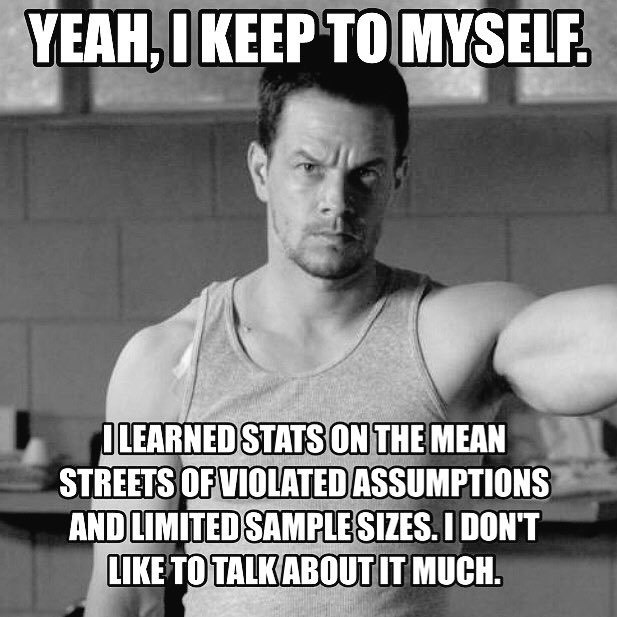
\includegraphics[width=0.7\linewidth]{figures/walberg_assumptions}

This is a workshop about the practice of the basic statistics used by
biologists, and not about the theory and mathematical underpinnings of
the methods used. Each of the Chapters will cover a basic kind of
statistical approach, and the main classes of data it applies to. Since
much insight and understanding can be gained from visualising our data,
we will also explore the main types of graphical summaries that best
accompany the statistical methodologies. It is our intention to
demonstrate how we go about analysing our data.

\hypertarget{prerequisites}{%
\chapter*{Prerequisites}\label{prerequisites}}


A prerequisite for this course is a basic proficiency in using R
\citep{R2017}. The necessary experience will have been gained from
completing the
\href{https://robwschlegel.github.io/Intro_R_Workshop/}{Intro R
Workshop: Data Manipulation, Analysis, and Graphing} Workshop that was
part of your BCB Core Honours module (i.e.~Biostatistics). You will also
need a laptop with R and RStudio installed as per the instructions
provided in that workshop. If you do not have a personal laptop, most
computers in the 5th floor lab will be correctly set up for this
purpose.

\hypertarget{introduction}{%
\chapter{Introduction}\label{introduction}}

\begin{quote}
\emph{\enquote{A scientist worthy of a lab coat should be able to make
original discoveries while wearing a clown suit, or give a lecture in a
high squeaky voice from inhaling helium. It is written nowhere in the
math of probability theory that one may have no fun.}}

--- Eliezer Yudkowsky
\end{quote}

\begin{quote}
\emph{\enquote{Prediction is very difficult, especially about the
future.}}

---- Niels Bohr
\end{quote}

\hypertarget{venue-date-and-time}{%
\section{Venue, date and time}\label{venue-date-and-time}}

Basic Statistics is the second half of the BSc (Hons) Biostats core
module, and will run from 12 April to 26 April 2018. This workshop will
take place on Tuesdays from \textbf{13:00--17:00}, Thursdays from
\textbf{10:40--17:00}, and Fridays from \textbf{08:30--17:00}. There
will be an assignment due about six weeks after the end of this module,
and it will provide the other half of the marks for the Biostats module.
More on the assignment later.

\hypertarget{course-outline}{%
\section{Course outline}\label{course-outline}}

\begin{enumerate}
\def\labelenumi{\arabic{enumi}.}
\tightlist
\item
  Introduction (this chapter)
\item
  Types of data
\item
  Descriptive statistics: Measures of location and dispersion
\item
  Representing data graphically
\item
  Distributions
\item
  One-sample and two-sample tests
\item
  Multi-sample (\textgreater{}2) tests
\item
  Linear regression
\item
  Correlation
\item
  Confidence intervals
\item
  Transforming data
\item
  Generalised linear model (GLM)
\item
  Chi square tests
\end{enumerate}

The course content can broadly be classified into two parts:
\emph{Descriptive Statistics} and \emph{Inferential Statistics}.

Descriptive statistics and their associated statistical and graphical
data summaries will be covered in Chapters 3 and 4. In Chapter 5 we will
introduce the concepts of data distributions, knowledge of which is
required to select the most appropriate inferential statistical methods.

Chapters 6-15 are about inferential statistics. Inferential tests allow
us to evaluate hypotheses within a framework of probabalistic theory,
which helps us infer the nature of a \enquote{population} based on a
smaller represenative set of samples. In partiucular, we can infer
whether the property under scrutiny (arrived at by means of a designed
experiment or a directed sampling programme) occured as a result of
deterministic influences, or whether it is as a result of chance.

\hypertarget{about-this-workshop}{%
\section{About this Workshop}\label{about-this-workshop}}

The aim of this workshop is to guide you through the outline given
above. The workshop focuses broadly (and unequally) on three groups of
concepts:

\begin{itemize}
\tightlist
\item
  Data and distributions
\item
  Descriptive statistics and graphics
\item
  Inferential statistics
\end{itemize}

Data and distributions are unsurprisingly about the data itself. Here we
will talk about the various kinds of data that we will encounter as
biologists. In the second part we will describe the data using a
combination of numerical and graphical summaries. Third, all of this
culminates in trying to infer from a small subset (a sample) of subjects
if the characteristics under scrutiny also hold true for the entire
population. We may also ask questions about probailities, i.e.~measuring
the likelihood that an event will occur, or that an experiment has an
outcome that is different from a situation where the influential
factor(s) has no effect, or that some observation or outcome is
non-random.

\hypertarget{this-is-biology-why-more-r-coding}{%
\section{This is biology: why more R
coding?}\label{this-is-biology-why-more-r-coding}}

Please refer to the
\href{https://robwschlegel.github.io/Intro_R_Workshop/}{Intro R
Workshop: Data Manipulation, Analysis and Graphing} for why we feel
strongly that you use R \citep{R2017} for the analyses that we will
perform here. All of the reasons provided there are valid here too, but
one reason perhaps more so than others---R and RStudio promote the
principles of \emph{reproducible research}, and in fact make it very
easy to implement. We will focus on some of these principles throughout
the workshop, and the assignments will require that you submit a fully
functional working script, complete with all the notes, memos, examples,
data, executable code, and output that will result from completing the
course material.

What other options are there for analysing the kinds of data that we
will encounter in biological research? Software packages like the ones
you may be familiar with, such as Statistica and SPSS, are often used to
perform many of these analyses. They are rather limited with regards to
the full scope of modern statistical methods in use by biologists today,
but many people still use these kinds of software as they provide the
basic kinds analyses that still form the staple of the biological and
medical sciences. For the many reasons provided above, we prefer to use
R as the \emph{engine} within which to do our biological data analysis.
R is used by academic statisticians the world over, and it is therefore
an excellent choice for our purpose here.

\hypertarget{installing-r-and-rstudio}{%
\section{Installing R and RStudio}\label{installing-r-and-rstudio}}

We assume that you already have R installed on your computer, as all of
you will have already completed the the Intro R Workshop. If you need a
refresher, please refer to
\href{https://robwschlegel.github.io/Intro_R_Workshop/}{Intro R
Workshop: Data Manipulation, Analysis and Graphing} for the installation
instructions.

\hypertarget{resources}{%
\section{Resources}\label{resources}}

\begin{itemize}
\tightlist
\item
  New users should introduce themselves to the
  \href{fg2re.sellorm.com}{R ecosystem}
\item
  A fancy interactive website that covers a wide range of
  \href{http://students.brown.edu/seeing-theory/}{basic statistics}
\item
  An easy to follow walkthrough for a
  \href{http://www.sthda.com/english/wiki/unpaired-two-samples-t-test-in-r}{statistical
  analysis}
\item
  Learn more about \href{https://infer.netlify.com}{tidy statistical
  inference}
\item
  A thorough journey through the philosophy of
  \href{http://www.serialmentor.com/dataviz/}{data visualisation}
\item
  \href{www.google.com}{Google}
\item
  \href{www.stackoverflow.com}{Stack Overflow}
\end{itemize}

\hypertarget{style-and-code-conventions}{%
\section{Style and code conventions}\label{style-and-code-conventions}}

Early on, develop the habit of unambiguous and consistent style and
formatting when writing your code, or anything else for that matter. Pay
attention to detail and be pedantic. This will benefit your scientific
writing in general. Although many R commands rely on precisely formatted
statements (code blocks), style can nevertheless to \emph{some extent}
have a personal flavour to it. The key is \emph{consistency}. In this
book we use certain conventions to improve readability. We also use a
consistent set of conventions to refer to code, and in particular to
typed commands and package names.

\begin{itemize}
\tightlist
\item
  Package names are shown in a bold font over a grey box, \emph{e.g.}
  \textbf{\texttt{tidyr}}.
\item
  Functions are shown in normal font followed by parentheses and also
  over a grey box , \emph{e.g.} \texttt{plot()}, or \texttt{summary()}.
\item
  Other R objects, such as data, function arguments or variable names
  are again in normal font over a grey box, but without parentheses,
  \emph{e.g.} \texttt{x} and \texttt{apples}.
\item
  Sometimes we might directly specify the package that contains the
  function by using two colons, \emph{e.g.} \texttt{dplyr::filter()}.
\item
  Commands entered onto the R command line (console) and the output that
  is returned will be shown in a code block, which is a light grey
  background with code font. The commands entered start at the beginning
  of a line and the output it produces is preceded by
  \texttt{R\textgreater{}}, like so:
\end{itemize}

\begin{Shaded}
\begin{Highlighting}[]
\KeywordTok{set.seed}\NormalTok{(}\DecValTok{666}\NormalTok{)}
\KeywordTok{rnorm}\NormalTok{(}\DataTypeTok{n =} \DecValTok{10}\NormalTok{, }\DataTypeTok{mean =} \DecValTok{0}\NormalTok{, }\DataTypeTok{sd =} \DecValTok{13}\NormalTok{)}
\end{Highlighting}
\end{Shaded}

\begin{verbatim}
R>  [1]   9.7930436  26.1866107  -4.6167480  26.3661820 -28.8193679
R>  [6]   9.8591503 -16.9804084 -10.4327544 -23.2991308  -0.5464219
\end{verbatim}

Consult these resources for more about R code style :

\begin{itemize}
\tightlist
\item
  \href{https://google.github.io/styleguide/Rguide.xml}{Google's R style
  guide}
\item
  \href{http://style.tidyverse.org}{The tidyverse style guide}
\item
  \href{http://adv-r.had.co.nz/Style.html}{Hadley Wickham's advanced R
  style guide}
\end{itemize}

We may also insert maths expressions within the text, like this
\(f(k) = {n \choose k} p^{k} (1-p)^{n-k}\) or on their own, like this:
\[f(k) = {n \choose k} p^{k} (1-p)^{n-k}\]

\hypertarget{assessment-and-teaching-philosophy}{%
\section{Assessment and teaching
philosophy}\label{assessment-and-teaching-philosophy}}

Grades will be based on the aggregate performance across two group
projects; the first group project was completed after the Intro R
Workshop. The project for this workshop will represent 35\% of the total
grade for BioStatistics. The remaining 15\% will come from daily
participation. This will be assessed by the R scripts produced in class
and follows these five criteria:

\begin{itemize}
\tightlist
\item
  The script has been uploaded to GitHub
\item
  The script covers the content of the day
\item
  The code runs without errors
\item
  Proper style conventions have been observed
\item
  Liberally commented
\end{itemize}

\textbf{BONUS POINTS}

\begin{itemize}
\tightlist
\item
  Additional analysis not performed in class
\item
  Additional figure not created in class
\end{itemize}

In cases where students are borderline between lower and higher grades,
a high level of participation in the class discussions and class in
general will win the day for the higher grade.

The daily scripts are essential to understanding the material. Although
they comprise only 15\% of the final grade, performance on the projects
is usually correlated with effort on the daily assignments.

Whereas plagiarism will not be tolerated, students ARE encouraged to
work together to learn from one another and solve problems in a
collaborative and collegial way.

\hypertarget{about-this-document}{%
\section{About this document}\label{about-this-document}}

This document, which as available as an HTML file that's viewable on a
web browser of your choice (anything will do, but we discourage using
Internet Explorer) and as a PDF (accessible from the link at the top of
any of the website's pages) that may be printed, was prepared by the
software tools available to R via RStudio. We use the package called
\texttt{bookdown} that may be accessed and read about
\href{https://bookdown.org/yihui/bookdown/}{here} to produce this
documentation. The entire source code to reproduce this book is
available from my \href{https://github.com/ajsmit/Basic_stats}{GitHub
repo}.

You will notice that this repository uses
\href{https://github.com}{GitHub}, and you are advised to set up your
own repository for R scripts and all your data. We will touch on GitHub
and the principles of reproducible research later, and GitHub forms a
core ingredient of such a workflow.

\hypertarget{types-of-data}{%
\chapter{Types of data}\label{types-of-data}}

\begin{quote}
\emph{\enquote{The plural of anecdote is not data.}}

--- Roger Brinner
\end{quote}

In this chapter we will, firstly, look at the different kinds of
biological and environmental data that are typically encountered by most
biologists. The data seen here are not an exhaustive list of all the
various types of data out there, but it should represent the bulk of our
needs.

After we have become familiar with the different kinds of data, we will
look at summaries of these data, which is generally required as the
starting point for our analyses. After summarising the data in tables
and so forth, we may want to produce graphical summaries to see broad
patterns and trends; visual data representations, which complement the
tabulated data, will be covered in a later chapter (Chapter 4). Both of
these approaches form the basis of \enquote{exploratory data analysis.}

\hypertarget{data-classes}{%
\section{Data classes}\label{data-classes}}

In biology we will encounter many kinds of data, and depending on which
kind, the type of statistical analysis will be decided.

\hypertarget{numerical-data}{%
\subsection{Numerical data}\label{numerical-data}}

Numerical data are quantitative in nature. They represent things that
can be objectively counted, measured or claculated.

\hypertarget{nominal-discrete-data}{%
\subsubsection{Nominal (discrete) data}\label{nominal-discrete-data}}

Integer data (discrete numbers or whole numbers), such as counts. For
example, family A may have 3 children and family B may have 1 child,
neither may have 2.3 children. Integer data usually answer the question,
\enquote{how many?} In R integer data are called \texttt{int} or
\texttt{\textless{}int\textgreater{}}.

\hypertarget{continuous-data}{%
\subsubsection{Continuous data}\label{continuous-data}}

These usually represent measured \enquote{things,} such as something's
heat content (temperature, measured in degrees Celsius) or distance
(measured in metres or similar), etc. They can be rational numbers
including integers and fractions, but typically they have an infinite
number of \enquote{steps} that depends on rounding (they can even be
rounded to whole integers) or considerations such as measurement
precision and accuracy. Often, continuous data have upper and lower
bounds that depend on the characteristics of the phenomenon being
studied or the measurement being taken. In R, continuous data are
denoted \texttt{num} or \texttt{\textless{}dbl\textgreater{}}.

The kinds of summaries that lend themselves to continuous data are:

\begin{itemize}
\tightlist
\item
  Frequency distributions
\item
  Relative frequency distributions
\item
  Cumulative frequency distributions
\item
  Bar graphs
\item
  Box plots
\item
  Scatter plots
\end{itemize}

\hypertarget{dates}{%
\subsubsection{Dates}\label{dates}}

Dates are a special class of continuous data, and there are many
different representations of the date classes. This is a complex group
of data, and we will not cover much of it in this course.

\hypertarget{qualitative-data}{%
\subsection{Qualitative data}\label{qualitative-data}}

Qualitative data may be well-defined categories or they may be
subjective, and generally include descriptive words for classes
(e.g.~mineral, animal , plant) or rankings (e.g.~good, better, best).

\hypertarget{categorical-data}{%
\subsubsection{Categorical data}\label{categorical-data}}

Because there are categories, the number of members belonging to each of
the categories can be counted. For example, there are three red flowers,
66 purple flowers, and 13 yellow flowers. The categories cannot be
ranked relative to each other; in the example just provided, for
instance, no value judgement can be assigned to the different colours.
It is not better to be red than it is to be purple. There are just fewer
red flowers than purple ones. Contrast this to another kind of
categorical data called \enquote{ordinal data} (see next). This class of
data in an R dataframe (or in a \enquote{tibble}) is indicated by
\texttt{Factor} or \texttt{\textless{}fctr\textgreater{}}.

The kinds of summaries that lend themselves to categorical data are:

\begin{itemize}
\tightlist
\item
  Frequency distributions
\item
  Relative frequency distributions
\item
  Bar graphs
\item
  Pie graphs (!!!)
\item
  Category statistics
\end{itemize}

\hypertarget{ordinal-data}{%
\subsubsection{Ordinal data}\label{ordinal-data}}

This is a type of categorical data where the classes are ordered (a
synonym is \enquote{ranked}), typically from low to high (or \emph{vice
versa}), but where the magnitude between the ordered classes cannot be
precisely measured or quantified. In other words, the difference between
them is somewhat subjective (i.e.~it is qualitative rather than
quantitative). These data are on an ordinal scale. The data may be
entered as descriptive character strings (i.e.~as words), or they may
have been translated to an ordered vector of integers; for example,
\enquote{1} for terrible, \enquote{2} for so-so, \enquote{3} for
average, \enquote{4} for good and \enquote{5} for brilliant.
Irrespective of how the data are present in the dataframe,
computationally (for some calculations) they are treated as an ordered
sequence of integers, but they are simultaneously treated as categories
(say, where the number of responses that report \enquote{so-so} can be
counted). Ordinal data usually answer questions such as, \enquote{how
many categories can the phenomenon be divided into, and how does each
category rank with respect to the others?} Columns containing this kind
of data are named \texttt{Ord.factor} or
\texttt{\textless{}ord\textgreater{}}.

\hypertarget{binary-data}{%
\subsection{Binary data}\label{binary-data}}

Right or wrong? True or false? Accept or reject? Black or white?
Positive or negative? Good or bad? You get the idea\ldots{} In other
words, these are observations or responses that can take only one of two
mutually exclusive outcomes. In R these are treated as \enquote{Logical}
data that take the values of \texttt{TRUE} or \texttt{FALSE} (note the
case). In R, and computing generally, logical data are often denoted
with 1 for \texttt{TRUE} and 0 for \texttt{FALSE}. This class of data is
indicated by \texttt{logi} or \texttt{\textless{}lgl\textgreater{}}.

\hypertarget{character-values}{%
\subsection{Character values}\label{character-values}}

As the name implies, these are not numbers. Rather, they are human words
that have found their way into R for one reason or another. In biology
we most commonly encounter character values when we have a list of
things, such as sites or species. These values will often be used as
categorical or ordinal data.

\hypertarget{missing-values}{%
\subsection{Missing values}\label{missing-values}}

Unfortunately, one of the most reliable aspects of any biological
dataset is that it will contain some missing data. But how can something
contain missing data? One could be forgiven for assuming that if the
data are missing, then they obviously aren't contained in the dataset.
TO better understand this concept we must think back to the principles
of tidy data. Every observation must be in a row, and every column in
that row must contain a value. The combination of multiple observations
then makes up our matrix of data. Because data are therefore presented
in a two-dimensional format, any missing values from an observation will
need to have an empty place-holder to ensure the consistency of the
matrix. These are waht we are referring to when we speak of
\enquote{missing values}. In R these appear as a \texttt{NA} in a
dataframe and are slighlty lighter than the other values. These data are
indicated in the Environment as \texttt{NA} and if a column contains
only missing values it will be denoted as
\texttt{\textless{}NA\textgreater{}}.

\hypertarget{complex-numbers}{%
\subsection{Complex numbers}\label{complex-numbers}}

\begin{quote}
\emph{\enquote{And if you gaze long enough into an abyss, the abyss will
gaze back into you.}}

--- Friedrich Nietzsche
\end{quote}

In an attempt to allow the shreds of our sanity to remain stitched
together we will end here with data types. But be warned, ye who enter,
that below countless rocks, and around a legion of corners, lay in wait
a myriad of complex data types. We will encounter many of these at the
end of this course when we encounter modeling, but by then we will have
learned a few techniques that will prepare us for the encounter.

\hypertarget{viewing-our-data}{%
\section{Viewing our data}\label{viewing-our-data}}

There are many ways of finding broad views of our data in R. The first
few functions that we will look at were designed to simply scrutinise
the contents of the tibbles, which is the \enquote{tidyverse} name for
the general \enquote{container} that holds our data in the software's
environment (i.e.~in a block of the computer's memory dedicated to the R
software). Whatever data are in R's environment will be seen in the
\enquote{Environment} tab in the top right of RStudio's four panes.

\hypertarget{from-the-environment-pane}{%
\subsection{From the Environment pane}\label{from-the-environment-pane}}

The first way to see what's in the tibble is not really a function at
all, but a convenient (and lazy) way of quickly seeing a few basic
things about our data. Let us look at the \texttt{ChickWeight} data.
Load it like so (you'll remember from the Intro R Workshop):

\begin{Shaded}
\begin{Highlighting}[]
\CommentTok{# loads the tidyverse functions; it contains the 'as_tibble()' function}
\KeywordTok{library}\NormalTok{(tidyverse)}
\CommentTok{# the 'ChickWeight' data are built into R;}
\CommentTok{# here we assign it as a tibble to an object named 'chicks'}
\NormalTok{chicks <-}\StringTok{ }\KeywordTok{as_tibble}\NormalTok{(ChickWeight)}
\end{Highlighting}
\end{Shaded}

In the Environment pane, the object named \texttt{chicks} will now
appear under the panel named Data. To the left of it is a small white
arrow in a blue circular background. By default the arrow points to the
right. Clicking on it causes it to point down, which denotes that the
data contained within the tibble have become expanded. The names of the
columns (more correctly called \enquote{variables}) can now be seen.
There you can see the variables \texttt{weight}, \texttt{Time},
\texttt{Chick} and \texttt{Diet}. The class of data they represent can
be seen too: there's continuous data of class \texttt{num}, a variable
of \texttt{Ord.factor}, and a categorical variable of class
\texttt{Factor}. Beneath these there's a lot of attributes that denote
some meta-data, which you may safely ignore for now.

\begin{figure}[h!]
\begin{center}
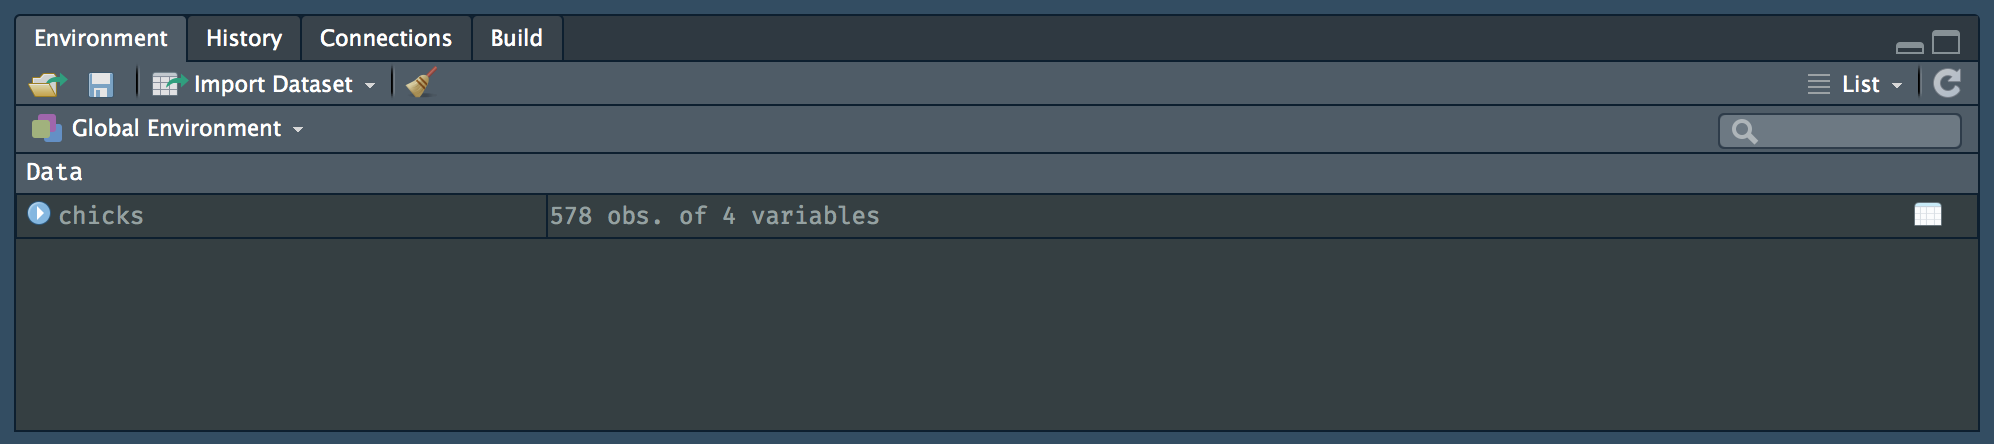
\includegraphics[width=0.7\linewidth]{figures/chicks_1}
\end{center}
\caption{What is in the Chicks data?}
\end{figure}

\begin{figure}[h!]
\begin{center}
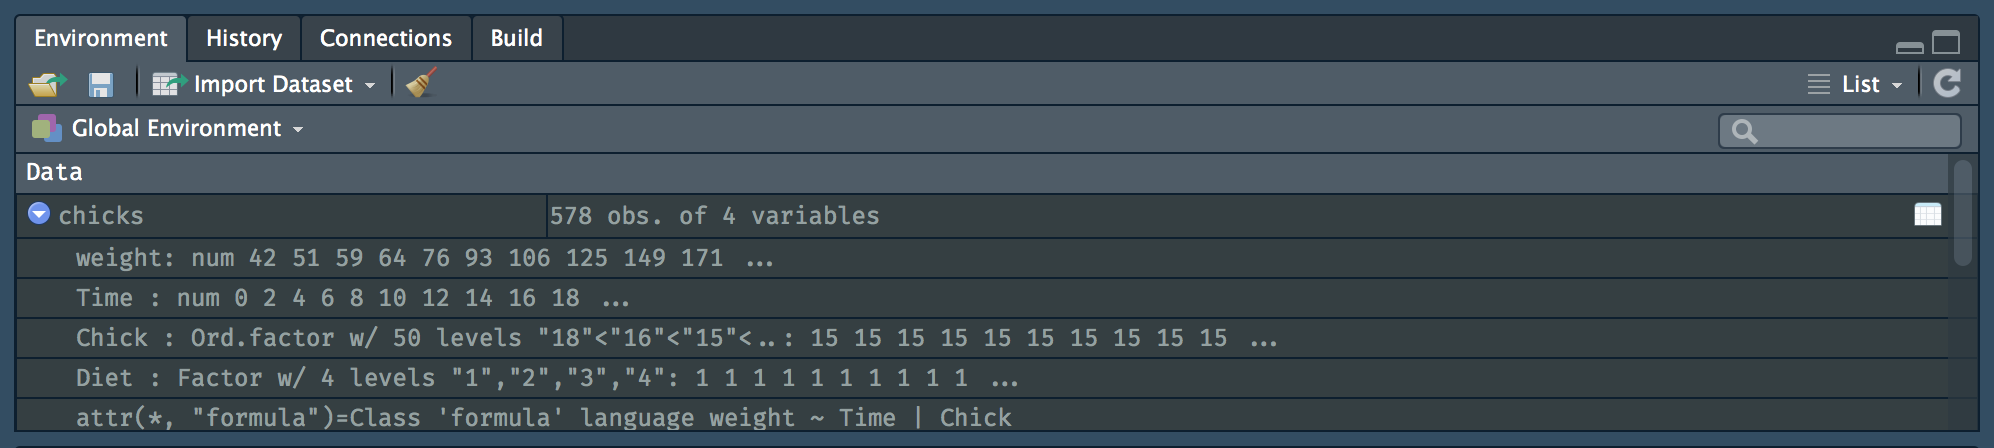
\includegraphics[width=0.7\linewidth]{figures/chicks_2}
\end{center}
\caption{This is what is in the Chicks data.}
\end{figure}

\hypertarget{head-and-tail}{%
\subsection{\texorpdfstring{\texttt{head()} and
\texttt{tail()}}{head() and tail()}}\label{head-and-tail}}

The \texttt{head()} and \texttt{tail()} functions simply display top and
bottom portions of the tibble, and you may add the \texttt{n} argument
and an integer to request that only a certain number of rows are
returned; by default the top or bottom six rows are displayed.

There are various bits of additional information printed out. The
display will change somewhat if there are many more variables than that
which can comfortably fit within the width of the output window
(typically the Console). The same kinds of information as was returned
with the Environment pane expansion arrow are displayed, but the data
class is now accompanied by an angle bracket (i.e.
\texttt{\textless{}...\textgreater{}}) notation. For example,
\texttt{num} in the Environment pane and
\texttt{\textless{}dbl\textgreater{}} as per the \texttt{head()} or
\texttt{tail()} methods are exactly the same: both denote continuous (or
\enquote{double precision}) data.

\begin{Shaded}
\begin{Highlighting}[]
\KeywordTok{head}\NormalTok{(chicks)}
\end{Highlighting}
\end{Shaded}

\begin{verbatim}
R> # A tibble: 6 x 4
R>   weight  Time Chick Diet 
R>    <dbl> <dbl> <ord> <fct>
R> 1    42.    0. 1     1    
R> 2    51.    2. 1     1    
R> 3    59.    4. 1     1    
R> 4    64.    6. 1     1    
R> 5    76.    8. 1     1    
R> 6    93.   10. 1     1
\end{verbatim}

\begin{Shaded}
\begin{Highlighting}[]
\KeywordTok{tail}\NormalTok{(chicks, }\DataTypeTok{n =} \DecValTok{2}\NormalTok{)}
\end{Highlighting}
\end{Shaded}

\begin{verbatim}
R> # A tibble: 2 x 4
R>   weight  Time Chick Diet 
R>    <dbl> <dbl> <ord> <fct>
R> 1   264.   20. 50    4    
R> 2   264.   21. 50    4
\end{verbatim}

As an alternative to \texttt{head()}, you may also simply type the name
of the object (here \texttt{chicks}) in the Console (or write it in the
Source Editor if it is necessary to retain the function for future use)
and the top portion of the tibble will be displayed, again trimmed to
account for the width of the display.

\hypertarget{colnames}{%
\subsection{\texorpdfstring{\texttt{colnames()}}{colnames()}}\label{colnames}}

This function simply returns a listing of the variable (column) names.

\begin{Shaded}
\begin{Highlighting}[]
\KeywordTok{colnames}\NormalTok{(chicks)}
\end{Highlighting}
\end{Shaded}

\begin{verbatim}
R> [1] "weight" "Time"   "Chick"  "Diet"
\end{verbatim}

There is an equivalent function called \texttt{rownames()} that may be
used to show the names of rows in your tibble, if these are present. Row
names are generally discouraged, and we will refrain from using them
here.

\hypertarget{summary}{%
\subsection{\texorpdfstring{\texttt{summary()}}{summary()}}\label{summary}}

The next way to see the contents of the tibble is to apply the
\texttt{summary()} function. Here we see something else. Some
descriptive statistics that describe properties of the full set of data
are now visible. These summary statistics condense each of the variables
into numbers that describe some properties of the data within each
column. You will already know the concepts of the \enquote{minimum,}
\enquote{median,} \enquote{mean,} and \enquote{maximum.} These are
displayed here.

\begin{Shaded}
\begin{Highlighting}[]
\KeywordTok{summary}\NormalTok{(chicks)}
\end{Highlighting}
\end{Shaded}

\begin{verbatim}
R>      weight           Time           Chick     Diet   
R>  Min.   : 35.0   Min.   : 0.00   13     : 12   1:220  
R>  1st Qu.: 63.0   1st Qu.: 4.00   9      : 12   2:120  
R>  Median :103.0   Median :10.00   20     : 12   3:120  
R>  Mean   :121.8   Mean   :10.72   10     : 12   4:118  
R>  3rd Qu.:163.8   3rd Qu.:16.00   17     : 12          
R>  Max.   :373.0   Max.   :21.00   19     : 12          
R>                                  (Other):506
\end{verbatim}

This will serve well as an introduction to the next chapter, which is
about descriptive statistics. What are they, and how do we calculate
them?

\hypertarget{descriptive-statistics-central-tendency-and-dispersion}{%
\chapter{Descriptive statistics: central tendency and
dispersion}\label{descriptive-statistics-central-tendency-and-dispersion}}

\begin{quote}
\emph{\enquote{I think it is much more interesting to live with
uncertainty than to live with answers that might be wrong.}}

---- Richard Feynman
\end{quote}

In this Chapter we will focus on basic descriptions of the data, and
these initial forrays are built around measures of the central tendency
of the data (the mean, median, mode) and the dispersion and variability
of the data (standard deviations and their ilk). The materials covered
in this and the next two chapters concern a broad discussion that will
aid us in understanding our data better prior to analysing it, and
before we can draw inference from it. In this work flow it emerges that
descriptive statistics generally precede inferential statistics.

Let us now turn to some of the most commonly used descriptive
statistics, and learn about how to calculate them.

\hypertarget{samples-and-populations}{%
\section{Samples and populations}\label{samples-and-populations}}

This is a simple toy example. In real life, however, our data will be
available in a tibble (initially perhaps captured in MS Excel before
importing it as a \texttt{.csv} file into R, where the tibble is
created). To see how this can be done more realistically using actual
data, let us turn to the ChickenWeight data, which, as before, we place
in the object \texttt{chicks}. Recall the pipe operator
(\texttt{\%\textgreater{}\%}, pronounced \enquote{then}) that we
introduced in the Intro R Workshop---we will use that here, throughout.
Let us calculate the sample size:

To determine the sample size we can use the \texttt{length()} or
\texttt{n()} functions; the latter is for use within \textbf{dplyr}'s
\texttt{summarise()} method, and it is applied without writing anything
inside of the \texttt{()}, like this:

\begin{Shaded}
\begin{Highlighting}[]
\CommentTok{# first load the tidyverse packages that has the pipe operator, %>%}
\KeywordTok{library}\NormalTok{(tidyverse)}
\NormalTok{chicks <-}\StringTok{ }\KeywordTok{as_tibble}\NormalTok{(ChickWeight)}

\CommentTok{# how many weights are available across all Diets and Times?}
\NormalTok{chicks }\OperatorTok\StringTok{ }
\StringTok{  }\KeywordTok{summarise}\NormalTok{(}\DataTypeTok{length =} \KeywordTok{n}\NormalTok{())}
\end{Highlighting}
\end{Shaded}

\begin{verbatim}
R> # A tibble: 1 x 1
R>   length
R>    <int>
R> 1    578
\end{verbatim}

\begin{Shaded}
\begin{Highlighting}[]
\CommentTok{# the same as}
\KeywordTok{length}\NormalTok{(chicks}\OperatorTok{$}\NormalTok{weight)}
\end{Highlighting}
\end{Shaded}

\begin{verbatim}
R> [1] 578
\end{verbatim}

Note that this gives us the number of all of the chicks in the
experiment, irrespective oif which diet they were given. It will make
more sense to know how many chicks were assigned to each of the
experimental diets they were raised on.

\begin{quote}
\textbf{Task:} Figure out the number of chicks in each of the feed
categories.
\end{quote}

\hypertarget{measures-of-central-tendency}{%
\section{Measures of central
tendency}\label{measures-of-central-tendency}}

\begin{longtable}[]{@{}lll@{}}
\caption{Measures of central tendency.}\tabularnewline
\toprule
\begin{minipage}[b]{0.25\columnwidth}\raggedright
Statistic\strut
\end{minipage} & \begin{minipage}[b]{0.18\columnwidth}\raggedright
Function\strut
\end{minipage} & \begin{minipage}[b]{0.18\columnwidth}\raggedright
Package\strut
\end{minipage}\tabularnewline
\midrule
\endfirsthead
\toprule
\begin{minipage}[b]{0.25\columnwidth}\raggedright
Statistic\strut
\end{minipage} & \begin{minipage}[b]{0.18\columnwidth}\raggedright
Function\strut
\end{minipage} & \begin{minipage}[b]{0.18\columnwidth}\raggedright
Package\strut
\end{minipage}\tabularnewline
\midrule
\endhead
\begin{minipage}[t]{0.25\columnwidth}\raggedright
Mean\strut
\end{minipage} & \begin{minipage}[t]{0.18\columnwidth}\raggedright
\texttt{mean()}\strut
\end{minipage} & \begin{minipage}[t]{0.18\columnwidth}\raggedright
\textbf{base}\strut
\end{minipage}\tabularnewline
\begin{minipage}[t]{0.25\columnwidth}\raggedright
Median\strut
\end{minipage} & \begin{minipage}[t]{0.18\columnwidth}\raggedright
\texttt{median()}\strut
\end{minipage} & \begin{minipage}[t]{0.18\columnwidth}\raggedright
\textbf{base}\strut
\end{minipage}\tabularnewline
\begin{minipage}[t]{0.25\columnwidth}\raggedright
Skewness\strut
\end{minipage} & \begin{minipage}[t]{0.18\columnwidth}\raggedright
\texttt{skewness()}\strut
\end{minipage} & \begin{minipage}[t]{0.18\columnwidth}\raggedright
\textbf{e1071}\strut
\end{minipage}\tabularnewline
\begin{minipage}[t]{0.25\columnwidth}\raggedright
Kurtosis\strut
\end{minipage} & \begin{minipage}[t]{0.18\columnwidth}\raggedright
\texttt{kurtosis()}\strut
\end{minipage} & \begin{minipage}[t]{0.18\columnwidth}\raggedright
\textbf{e1071}\strut
\end{minipage}\tabularnewline
\bottomrule
\end{longtable}

The measures of central tendency are also sometimes called
\enquote{location} statistics. We have already seen summaries of the
mean and the median when we called to \texttt{summary()} function on the
\texttt{chicks} data in Chapter 2. Here we shall show you how they can
be calculated using some built-in R functions.

\hypertarget{the-mean}{%
\subsection{The mean}\label{the-mean}}

The sample \emph{mean} is the arithmetic average of the data, and it is
calculated by summing all the data and dividing it by the sample size,
\emph{n}. The mean, \(\bar{x}\), is calculated thus:

\[\bar{x} = \frac{1}{n}\sum_{i=1}^{n}x_{i} = \frac{x_{1} + x_{2} + \cdots + x_{n}}{n}\]
where \(x_{1} + x_{2} + \cdots + x_{n}\) are the observations and \(n\)
is the number of observations in the sample.

In R one can quickly apply the \texttt{mean()} function to some data.
Let us create a vector of arbitrary numbers using the \enquote{combine}
function, \texttt{c()}, and then apply the function for the mean:

\begin{Shaded}
\begin{Highlighting}[]
\CommentTok{# combine a series of numbers into a vector;}
\CommentTok{# hint: use this function in the exercises that we will require from you}
\CommentTok{# later on...}
\NormalTok{dat1 <-}\StringTok{ }\KeywordTok{c}\NormalTok{(}\DecValTok{23}\NormalTok{, }\DecValTok{45}\NormalTok{, }\DecValTok{23}\NormalTok{, }\DecValTok{66}\NormalTok{, }\DecValTok{13}\NormalTok{)}
\KeywordTok{mean}\NormalTok{(dat1)}
\end{Highlighting}
\end{Shaded}

\begin{verbatim}
R> [1] 34
\end{verbatim}

Below, we use another tidyverse package, \textbf{\texttt{dplyr}} and its
\texttt{summarise()} function, whose purpose it is to \emph{summarise}
the entire column into one summary statistic, in this case the mean:

\begin{Shaded}
\begin{Highlighting}[]
\NormalTok{chicks }\OperatorTok\StringTok{ }
\StringTok{  }\KeywordTok{summarise}\NormalTok{(}\DataTypeTok{mean_wt =} \KeywordTok{mean}\NormalTok{(weight))}
\end{Highlighting}
\end{Shaded}

\begin{verbatim}
R> # A tibble: 1 x 1
R>   mean_wt
R>     <dbl>
R> 1    122.
\end{verbatim}

We can achieve the same using the more traditional syntax, which in some
instances may be slightly less verbose, but less user-friendly,
especially when multiple summary statistics are required (we shall later
on how we can summarise a vector of data into multiple statistics). The
traditional syntax is:

\begin{Shaded}
\begin{Highlighting}[]
\CommentTok{# the '$' operator is used to denote a variable inside of the tibble}
\KeywordTok{mean}\NormalTok{(chicks}\OperatorTok{$}\NormalTok{weight)}
\end{Highlighting}
\end{Shaded}

\begin{verbatim}
R> [1] 121.8183
\end{verbatim}

\begin{quote}
\textbf{Task:} How would you manually calculate the mean mass for the
chicks? Do it now!
\end{quote}

Notice above how the two approaches display the result differently: in
the first instance, using \texttt{summarise()}, the answer is rounded to
zero decimal places; in the second, it is displayed (here) at full
precision. The precision of the answer that you require depends on the
context of your study, so make sure that you use the appropriate number
of significant digits. Using the \texttt{summarise()} approach again,
here is how you can adjust the number of decimal places of the answer:

\begin{Shaded}
\begin{Highlighting}[]
\CommentTok{# the value printed in the HTML/PDF versions is incorrect;}
\CommentTok{# check in the console for correct output}
\NormalTok{chicks }\OperatorTok\StringTok{ }
\StringTok{  }\KeywordTok{summarise}\NormalTok{(}\DataTypeTok{mean_wt =} \KeywordTok{round}\NormalTok{(}\KeywordTok{mean}\NormalTok{(weight), }\DecValTok{1}\NormalTok{))}
\end{Highlighting}
\end{Shaded}

\begin{verbatim}
R> # A tibble: 1 x 1
R>   mean_wt
R>     <dbl>
R> 1    122.
\end{verbatim}

\begin{quote}
\textbf{Task:} What happens when there are missing values (\texttt{NA})?
Consult the help file for the \texttt{mean()} function, discuss amongst
yourselves, and then provide a demonstration to the class of how you
would handle missing values. Hint: use the \texttt{c()} function to
capture a series of data that you can then use to demonstrate your
understanding.
\end{quote}

At this point it might be useful to point out that the mean (or any
function for that matter, even one that does not yet exist) can be
programatically calculated. Let us demonstrate the principle by
reproducing the mean function from the constituent parts:

\begin{Shaded}
\begin{Highlighting}[]
\NormalTok{chicks }\OperatorTok\StringTok{ }
\StringTok{  }\KeywordTok{summarise}\NormalTok{(}\DataTypeTok{mean_wt =} \KeywordTok{sum}\NormalTok{(weight) }\OperatorTok{/}\StringTok{ }\KeywordTok{n}\NormalTok{())}
\end{Highlighting}
\end{Shaded}

\begin{verbatim}
R> # A tibble: 1 x 1
R>   mean_wt
R>     <dbl>
R> 1    122.
\end{verbatim}

The mean is quite sensitive to the presence of outliers or extreme
values in the data, and it is advised that its use be reserved for
normally distributed data from which the extremes/outliers have been
removed. When extreme values are indeed part of our data and not simply
\enquote{noise,} then we have to resort to a different measure of
central tendency: the median.

\begin{quote}
*Task:** In statistics, what do we mean with \enquote{noise}?
\end{quote}

\hypertarget{the-median}{%
\subsection{The median}\label{the-median}}

The \emph{median} can be calculated by \enquote{hand} (if you have a
small enough amount of data) by arranging all the numbers in sequence
from low to high, and then finding the middle value. If there are five
numbers, say \texttt{5,\ 2,\ 6,\ 13,\ 1}, then you would arrange them
from low to high, i.e. \texttt{1,\ 2,\ 5,\ 6,\ 13}. The middle number is
\texttt{5}. This is the median. But there is no middle if we have an
even number of values. What now? Take this example sequence of six
integers (they may also be floating point numbers), which has already
been ordered for your pleasure: \texttt{1,\ 2,\ 5,\ 6,\ 9,\ 13}. Find
the middle two numbers (i.e. \texttt{5,\ 6}) and take the mean. It is
\texttt{5.5}. That is the median.

Let us find the median for the weights of the chickens in the
ChickWeight data:

\begin{Shaded}
\begin{Highlighting}[]
\NormalTok{chicks }\OperatorTok\StringTok{ }
\StringTok{  }\KeywordTok{summarise}\NormalTok{(}\DataTypeTok{med_wt =} \KeywordTok{median}\NormalTok{(weight))}
\end{Highlighting}
\end{Shaded}

\begin{verbatim}
R> # A tibble: 1 x 1
R>   med_wt
R>    <dbl>
R> 1   103.
\end{verbatim}

The median is therefore the value that separates the lower half of the
sample data from the upper half. In normally distributed continuous data
the median is equal to the mean. Comparable concepts to the median are
the \emph{1st} and \emph{3rd quartiles}, which, respectively, separate
the first quarter of the data from the last quarter---see later. The
advantage of the median over the mean is that it is unaffected (i.e.~not
skewed) by extreme values or outliers, and it gives an idea of the
typical value of the sample. The median is also used to provide a robust
description of non-parametric data (see Chapter 4 for a discussion on
normal data and other data distributions).

\hypertarget{skewness}{%
\subsection{Skewness}\label{skewness}}

Skewness is a measure of symmetry, and it is best understood by
understanding the location of the median relative to the mean. A
negative skewness indicates that the mean of the data is less than their
median---the data distribution is left-skewed. A positive skewness
results from data that have a mean that is larger than their median;
these data have a right-skewed distribution.

\begin{Shaded}
\begin{Highlighting}[]
\KeywordTok{library}\NormalTok{(e1071)}
\KeywordTok{skewness}\NormalTok{(faithful}\OperatorTok{$}\NormalTok{eruptions)}
\end{Highlighting}
\end{Shaded}

\begin{verbatim}
R> [1] -0.4135498
\end{verbatim}

\begin{quote}
\textbf{Task:} Is the distribution left or right skewed?
\end{quote}

\hypertarget{kurtosis}{%
\subsection{Kurtosis}\label{kurtosis}}

Kurtosis describes the tail shape of the data's distribution. A normal
distribution has zero kurtosis and thus the standard tail shape
(mesokurtic). Negative kurtosis indicates data with a thin-tailed
(platykurtic) distribution. Positive kurtosis indicates a fat-tailed
distribution (leptokurtic).

\begin{Shaded}
\begin{Highlighting}[]
\CommentTok{# library(e1071)}
\KeywordTok{kurtosis}\NormalTok{(faithful}\OperatorTok{$}\NormalTok{eruptions)}
\end{Highlighting}
\end{Shaded}

\begin{verbatim}
R> [1] -1.511605
\end{verbatim}

\hypertarget{measures-of-variation-and-spread}{%
\section{Measures of variation and
spread}\label{measures-of-variation-and-spread}}

Since the mean or median does not tell us everything there is to know
about data, we will also have to determine some statistics that inform
us about the variation (or spread or dispersal or inertia) around the
central/mean value.

\begin{longtable}[]{@{}ll@{}}
\caption{Measures of variation and spread.}\tabularnewline
\toprule
\begin{minipage}[b]{0.29\columnwidth}\raggedright
Statistic\strut
\end{minipage} & \begin{minipage}[b]{0.29\columnwidth}\raggedright
Function\strut
\end{minipage}\tabularnewline
\midrule
\endfirsthead
\toprule
\begin{minipage}[b]{0.29\columnwidth}\raggedright
Statistic\strut
\end{minipage} & \begin{minipage}[b]{0.29\columnwidth}\raggedright
Function\strut
\end{minipage}\tabularnewline
\midrule
\endhead
\begin{minipage}[t]{0.29\columnwidth}\raggedright
Variance\strut
\end{minipage} & \begin{minipage}[t]{0.29\columnwidth}\raggedright
\texttt{var()}\strut
\end{minipage}\tabularnewline
\begin{minipage}[t]{0.29\columnwidth}\raggedright
Standard deviation\strut
\end{minipage} & \begin{minipage}[t]{0.29\columnwidth}\raggedright
\texttt{sd()}\strut
\end{minipage}\tabularnewline
\begin{minipage}[t]{0.29\columnwidth}\raggedright
Minimum\strut
\end{minipage} & \begin{minipage}[t]{0.29\columnwidth}\raggedright
\texttt{min()}\strut
\end{minipage}\tabularnewline
\begin{minipage}[t]{0.29\columnwidth}\raggedright
Maximum\strut
\end{minipage} & \begin{minipage}[t]{0.29\columnwidth}\raggedright
\texttt{max()}\strut
\end{minipage}\tabularnewline
\begin{minipage}[t]{0.29\columnwidth}\raggedright
Range\strut
\end{minipage} & \begin{minipage}[t]{0.29\columnwidth}\raggedright
\texttt{range()}\strut
\end{minipage}\tabularnewline
\begin{minipage}[t]{0.29\columnwidth}\raggedright
Quantile\strut
\end{minipage} & \begin{minipage}[t]{0.29\columnwidth}\raggedright
\texttt{quantile()}\strut
\end{minipage}\tabularnewline
\begin{minipage}[t]{0.29\columnwidth}\raggedright
Covariance\strut
\end{minipage} & \begin{minipage}[t]{0.29\columnwidth}\raggedright
\texttt{cov()}\strut
\end{minipage}\tabularnewline
\begin{minipage}[t]{0.29\columnwidth}\raggedright
Correlation\strut
\end{minipage} & \begin{minipage}[t]{0.29\columnwidth}\raggedright
\texttt{cor()}\strut
\end{minipage}\tabularnewline
\bottomrule
\end{longtable}

\hypertarget{the-variance-and-standard-deviation}{%
\subsection{The variance and standard
deviation}\label{the-variance-and-standard-deviation}}

The variance and standard deviation are examples of interval estimates.
The \emph{sample variance}, \(S^{2}\), may be calculated according to
the following formula:

\[S^{2} = \frac{1}{n-1}\sum_{i=1}^{n}(x_{i}-\bar{x})^{2}\]

This reads: \enquote{the sum of the squared differences from the mean,
divided by the sample size minus 1.}

To get the \emph{standard deviation}, \(S\), we take the square root of
the variance, i.e. \(S = \sqrt{S^{2}}\).

No need to plug these equations into MS Excel. Let us quickly calculate
\(S\) in R. Again, we use the \texttt{chicks} data:

\begin{Shaded}
\begin{Highlighting}[]
\NormalTok{chicks }\OperatorTok\StringTok{ }
\StringTok{  }\KeywordTok{summarise}\NormalTok{(}\DataTypeTok{sd_wt =} \KeywordTok{sd}\NormalTok{(weight))}
\end{Highlighting}
\end{Shaded}

\begin{verbatim}
R> # A tibble: 1 x 1
R>   sd_wt
R>   <dbl>
R> 1  71.1
\end{verbatim}

The interpretation of the concepts of mean and median are fairly
straight forward and intuitive. Not so for the measures of variance.
What does \(S\) represent? Firstly, the unit of measurement of \(S\) is
the same as that of \(\bar{x}\) (but the variance doesn't share this
characteristic). If temperature is measured in °C, then \(S\) also takes
a unit of °C. Since \(S\) measures the dispersion \emph{around} the
mean, we write it as \(\bar{x} \pm S\) (note that often the mean and
standard deviation are written with the letters \emph{mu} and
\emph{sigma}, respectively; i.e. \(\mu \pm \sigma\)). The smaller \(S\)
the closer the sample data are to \(\bar{x}\), and the larger the value
is the further away they will spread out from \(\bar{x}\). So, it tells
us about the proportion of observations above and below \(\bar{x}\). But
what proportion? We invoke the the 68-95-99.7 rule:
\textasciitilde{}68\% of the population (as represented by a random
sample of \(n\) observations taken from the population) falls within
1\(S\) of \(\bar{x}\) (i.e. \textasciitilde{}34\% below \(\bar{x}\) and
\textasciitilde{}34\% above \(\bar{x}\)); \textasciitilde{}95\% of the
population falls within 2\(S\); and \textasciitilde{}99.7\% falls within
3\(S\).

\textbackslash{}begin\{figure\}{[}h!{]}

\begin{center}
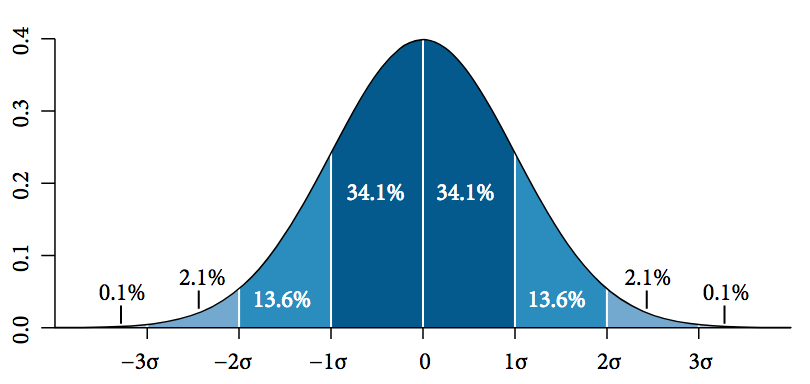
\includegraphics[width=0.7\linewidth]{figures/Standard_deviation_diagram.png}
\end{center}

\textbackslash{}caption\{The proportions of data representation by the
standard deviation. Credit: wikipedia/Standard\_deviation\}
\textbackslash{}end\{figure\}

Like the mean, \(S\) is affected by extreme values and outliers, so
before we attach \(S\) as a summary statistic to describe some data, we
need to ensure that the data are in fact normally distributed. We will
talk about how to do this in Chapter 6, where we will go over the
numerous ways to check the assumption of normality. When the data are
found to be non-normal, we need to find appropriate ways to express the
spread of the data. Enter the quartiles.

\hypertarget{quantiles}{%
\subsection{Quantiles}\label{quantiles}}

A more forgiving approach (forgiving of the extremes, often called
\enquote{robust}) is to divide the distribution of ordered data into
quarters, and find the points below which 25\% (0.25, the first
quartile), 50\% (0.50, the median) and 75\% (0.75, the third quartile)
of the data are distributed. These are called \emph{quartiles} (for
\enquote{quarter;} not to be confused with \emph{quantile}, which is a
more general form of the function that can be used to divide the
distribution into any arbitrary proportion from 0 to 1). In R we use the
\texttt{quantile()} function to provide the quartiles; we demonstrate
two approaches:

\begin{Shaded}
\begin{Highlighting}[]
\KeywordTok{quantile}\NormalTok{(chicks}\OperatorTok{$}\NormalTok{weight)}
\end{Highlighting}
\end{Shaded}

\begin{verbatim}
R>     0%    25%    50%    75%   100% 
R>  35.00  63.00 103.00 163.75 373.00
\end{verbatim}

\begin{Shaded}
\begin{Highlighting}[]
\NormalTok{chicks }\OperatorTok\StringTok{ }
\StringTok{  }\KeywordTok{summarise}\NormalTok{(}\DataTypeTok{min_wt =} \KeywordTok{min}\NormalTok{(weight),}
            \DataTypeTok{qrt1_wt =} \KeywordTok{quantile}\NormalTok{(weight, }\DataTypeTok{p =} \FloatTok{0.25}\NormalTok{),}
            \DataTypeTok{med_wt =} \KeywordTok{median}\NormalTok{(weight),}
            \DataTypeTok{qrt3_wt =} \KeywordTok{median}\NormalTok{(weight, }\DataTypeTok{p =} \FloatTok{0.75}\NormalTok{),}
            \DataTypeTok{max_wt =} \KeywordTok{max}\NormalTok{(weight))}
\end{Highlighting}
\end{Shaded}

\begin{verbatim}
R> # A tibble: 1 x 5
R>   min_wt qrt1_wt med_wt qrt3_wt max_wt
R>    <dbl>   <dbl>  <dbl>   <dbl>  <dbl>
R> 1    35.     63.   103.    103.   373.
\end{verbatim}

\begin{Shaded}
\begin{Highlighting}[]
\CommentTok{# note median(weight) is the same as quantile(weight, p = 0.5) }
\CommentTok{# in the summarise() implementation, above}
\end{Highlighting}
\end{Shaded}

\begin{quote}
\emph{Task:} What is different about the \texttt{quantile()} function
that caused us to specify the calculation in the way in which we have
done so above? You will have to consult the help file, read it,
understand it, think about it, and experiment with the ideas. Take 15
minutes to figure it out and report back to the class.
\end{quote}

\hypertarget{the-minimum-maximum-and-range}{%
\subsection{The minimum, maximum and
range}\label{the-minimum-maximum-and-range}}

A description of the extent of the data can also be provided by the
functions \texttt{min()}, \texttt{max()} and \texttt{range()}.

These statistics apply to data of any distribution, and not only to
normal data. This if often the first place you want to start when
looking at the data for the first time. We've seen above how to use
\texttt{min()} and \texttt{max()}, so below we will quickly look at how
to use \texttt{range()} in both the base R and tidy methods:

\begin{Shaded}
\begin{Highlighting}[]
\KeywordTok{range}\NormalTok{(chicks}\OperatorTok{$}\NormalTok{weight)}
\end{Highlighting}
\end{Shaded}

\begin{verbatim}
R> [1]  35 373
\end{verbatim}

\begin{Shaded}
\begin{Highlighting}[]
\NormalTok{chicks }\OperatorTok\StringTok{ }
\StringTok{  }\KeywordTok{summarise}\NormalTok{(}\DataTypeTok{lower_wt =} \KeywordTok{range}\NormalTok{(weight)[}\DecValTok{1}\NormalTok{],}
            \DataTypeTok{upper_wt =} \KeywordTok{range}\NormalTok{(weight)[}\DecValTok{2}\NormalTok{])}
\end{Highlighting}
\end{Shaded}

\begin{verbatim}
R> # A tibble: 1 x 2
R>   lower_wt upper_wt
R>      <dbl>    <dbl>
R> 1      35.     373.
\end{verbatim}

Note that \texttt{range()} actually gives us the minimum and maximum
values, and not the difference between them. To find the range value
properly we must be a bit more clever:

\begin{Shaded}
\begin{Highlighting}[]
\KeywordTok{range}\NormalTok{(chicks}\OperatorTok{$}\NormalTok{weight)[}\DecValTok{2}\NormalTok{] }\OperatorTok{-}\StringTok{ }\KeywordTok{range}\NormalTok{(chicks}\OperatorTok{$}\NormalTok{weight)[}\DecValTok{1}\NormalTok{]}
\end{Highlighting}
\end{Shaded}

\begin{verbatim}
R> [1] 338
\end{verbatim}

\begin{Shaded}
\begin{Highlighting}[]
\NormalTok{chicks }\OperatorTok\StringTok{ }
\StringTok{  }\KeywordTok{summarise}\NormalTok{(}\DataTypeTok{range_wt =} \KeywordTok{range}\NormalTok{(weight)[}\DecValTok{2}\NormalTok{] }\OperatorTok{-}\StringTok{ }\KeywordTok{range}\NormalTok{(weight)[}\DecValTok{1}\NormalTok{])}
\end{Highlighting}
\end{Shaded}

\begin{verbatim}
R> # A tibble: 1 x 1
R>   range_wt
R>      <dbl>
R> 1     338.
\end{verbatim}

\hypertarget{covariance}{%
\subsection{Covariance}\label{covariance}}

\hypertarget{correlation}{%
\subsection{Correlation}\label{correlation}}

The correlation coefficient of two matched (paired) variables is equal
to their covariance divided by the product of their individual standard
deviations. It is a normalised measurement of how linearly related the
two variables are.

Graphical displays of correlations are provided by scatter plots as can
be seen in Section X.

\hypertarget{missing-values-1}{%
\section{Missing values}\label{missing-values-1}}

As mentioned in Chapter 2, missing data are pervaise in the biological
sciences. Happily for us, R is designed to handle these data easily. It
is important to note here explicitly that all of the basic functions in
R will by default \emph{NOT} ignore missing data. This has been done so
as to prevent the user from accidentally forgetting about the missing
data and potentially making errors in later stages in an analysis.
Therefore, we must explicitly tell R when we want it to ommit missing
values from a calculation. Let's create a small vector of data to
demonstrate this:

\begin{Shaded}
\begin{Highlighting}[]
\NormalTok{dat1 <-}\StringTok{ }\KeywordTok{c}\NormalTok{(}\OtherTok{NA}\NormalTok{, }\DecValTok{12}\NormalTok{, }\DecValTok{76}\NormalTok{, }\DecValTok{34}\NormalTok{, }\DecValTok{23}\NormalTok{)}

\CommentTok{# Without telling R to ommit missing data}
\KeywordTok{mean}\NormalTok{(dat1)}
\end{Highlighting}
\end{Shaded}

\begin{verbatim}
R> [1] NA
\end{verbatim}

\begin{Shaded}
\begin{Highlighting}[]
\CommentTok{# Ommitting the missing data}
\KeywordTok{mean}\NormalTok{(dat1, }\DataTypeTok{na.rm =} \OtherTok{TRUE}\NormalTok{)}
\end{Highlighting}
\end{Shaded}

\begin{verbatim}
R> [1] 36.25
\end{verbatim}

Note that this argument, \texttt{na.rm\ =\ TRUE} may be used in all of
the functions we have seen thus far in this chapter.

\hypertarget{descriptive-statistics-by-group}{%
\section{Descriptive statistics by
group}\label{descriptive-statistics-by-group}}

Above we have revised the basic kinds of summary statistics, and how to
calculate them. This is nice. But it can be more useful. The real reason
why we might want to see the descriptive statistics is to facilitate
comparisons between groups. In the chicks data we calculated the mean
(etc.) for all the chickens, over all the diet groups to which they had
been assigned (there are four factors, i.e.~Diets 1 to 4), and over the
entire duration of the experiment (the experiment lasted 21 days). It
would be more useful to see what the weights are of the chickens in each
of the four groups at the end of the experiment --- we can compare means
(± SD) and medians (± interquartile ranges, etc.), for instance. You'll
notice now how the measures of central tendency is being combined with
the measures of variability/range. Further, we can augment this
statistical summary with many kinds of graphical summaries, which will
be far more revealing of differences (if any) amongst groups. We will
revise how to produce the group statistics and show a range of graphical
displays.

\hypertarget{groupwise-summary-statistics}{%
\subsection{Groupwise summary
statistics}\label{groupwise-summary-statistics}}

At this point you need to refer to
\href{https://robwschlegel.github.io/Intro_R_Workshop/tidy.html}{Chapter
10} (Tidy data) and
\href{https://robwschlegel.github.io/Intro_R_Workshop/tidier.html}{Chapter
11} (Tidier data) in the \textbf{Intro R Workshop} to remind yourself
about in what format the data need to be before we can efficiently work
with it. A hint: one observation in a row, and one variable per column.
From this point, it is trivial to do the various data descriptions,
visualisations, and analyses. Thankfully, the \texttt{chicks} data are
already in this format.

So, what are the summary statistics for the chickens for each diet group
at day 21?

\begin{Shaded}
\begin{Highlighting}[]
\NormalTok{grp_stat <-}\StringTok{ }\NormalTok{chicks }\OperatorTok
\StringTok{  }\KeywordTok{filter}\NormalTok{(Time }\OperatorTok{==}\StringTok{ }\DecValTok{21}\NormalTok{) }\OperatorTok\StringTok{ }
\StringTok{  }\KeywordTok{group_by}\NormalTok{(Diet, Time) }\OperatorTok\StringTok{ }
\StringTok{  }\KeywordTok{summarise}\NormalTok{(}\DataTypeTok{mean_wt =} \KeywordTok{round}\NormalTok{(}\KeywordTok{mean}\NormalTok{(weight, }\DataTypeTok{na.rm =} \OtherTok{TRUE}\NormalTok{), }\DecValTok{2}\NormalTok{),}
            \DataTypeTok{med_wt =} \KeywordTok{median}\NormalTok{(weight, }\DataTypeTok{na.rm =} \OtherTok{TRUE}\NormalTok{),}
            \DataTypeTok{sd_wt =} \KeywordTok{round}\NormalTok{(}\KeywordTok{sd}\NormalTok{(weight, }\DataTypeTok{na.rm =} \OtherTok{TRUE}\NormalTok{), }\DecValTok{2}\NormalTok{),}
            \DataTypeTok{sum_wt =} \KeywordTok{sum}\NormalTok{(weight),}
            \DataTypeTok{min_wt =} \KeywordTok{min}\NormalTok{(weight),}
            \DataTypeTok{qrt1_wt =} \KeywordTok{quantile}\NormalTok{(weight, }\DataTypeTok{p =} \FloatTok{0.25}\NormalTok{),}
            \DataTypeTok{med_wt =} \KeywordTok{median}\NormalTok{(weight),}
            \DataTypeTok{qrt3_wt =} \KeywordTok{median}\NormalTok{(weight, }\DataTypeTok{p =} \FloatTok{0.75}\NormalTok{),}
            \DataTypeTok{max_wt =} \KeywordTok{max}\NormalTok{(weight),}
            \DataTypeTok{n_wt =} \KeywordTok{n}\NormalTok{())}
\NormalTok{grp_stat}
\end{Highlighting}
\end{Shaded}

\begin{verbatim}
R> # A tibble: 4 x 11
R> # Groups:   Diet [?]
R>   Diet   Time mean_wt med_wt sd_wt sum_wt min_wt qrt1_wt qrt3_wt max_wt
R>   <fct> <dbl>   <dbl>  <dbl> <dbl>  <dbl>  <dbl>   <dbl>   <dbl>  <dbl>
R> 1 1       21.    178.   166.  58.7  2844.    96.    138.    166.   305.
R> 2 2       21.    215.   212.  78.1  2147.    74.    169.    212.   331.
R> 3 3       21.    270.   281.  71.6  2703.   147.    229.    281.   373.
R> 4 4       21.    239.   237.  43.4  2147.   196.    204.    237.   322.
R> # ... with 1 more variable: n_wt <int>
\end{verbatim}

\hypertarget{displays-of-group-summaries}{%
\subsection{Displays of group
summaries}\label{displays-of-group-summaries}}

There are several kinds of graphical displays for your data. We will
show some which are able to display the spread of the raw data, the mean
or median, as well as the appropriate accompanying indicators of
variation around the mean or median.

\begin{Shaded}
\begin{Highlighting}[]
\KeywordTok{library}\NormalTok{(ggpubr) }\CommentTok{# needed for arranging multi-panel plots}
\NormalTok{plt1 <-}\StringTok{ }\NormalTok{chicks }\OperatorTok
\StringTok{  }\KeywordTok{filter}\NormalTok{(Time }\OperatorTok{==}\StringTok{ }\DecValTok{21}\NormalTok{) }\OperatorTok\StringTok{ }
\StringTok{  }\KeywordTok{ggplot}\NormalTok{(}\KeywordTok{aes}\NormalTok{(}\DataTypeTok{x =}\NormalTok{ Diet, }\DataTypeTok{y =}\NormalTok{ weight)) }\OperatorTok{+}
\StringTok{  }\KeywordTok{geom_point}\NormalTok{(}\DataTypeTok{data =}\NormalTok{ grp_stat, }\KeywordTok{aes}\NormalTok{(}\DataTypeTok{x =}\NormalTok{ Diet, }\DataTypeTok{y =}\NormalTok{ mean_wt), }
             \DataTypeTok{col =} \StringTok{"black"}\NormalTok{, }\DataTypeTok{fill =} \StringTok{"red"}\NormalTok{, }\DataTypeTok{shape =} \DecValTok{23}\NormalTok{, }\DataTypeTok{size =} \DecValTok{3}\NormalTok{) }\OperatorTok{+}
\StringTok{  }\KeywordTok{geom_jitter}\NormalTok{(}\DataTypeTok{width =} \FloatTok{0.05}\NormalTok{) }\OperatorTok{+}\StringTok{ }\CommentTok{# geom_point() if jitter not required}
\StringTok{  }\KeywordTok{labs}\NormalTok{(}\DataTypeTok{y =} \StringTok{"Chicken mass (g)"}\NormalTok{) }\OperatorTok{+}\StringTok{ }
\StringTok{  }\KeywordTok{theme_pubr}\NormalTok{()}

\NormalTok{plt2 <-}\StringTok{ }\KeywordTok{ggplot}\NormalTok{(}\DataTypeTok{data =}\NormalTok{ grp_stat, }\KeywordTok{aes}\NormalTok{(}\DataTypeTok{x =}\NormalTok{ Diet, }\DataTypeTok{y =}\NormalTok{ mean_wt)) }\OperatorTok{+}
\StringTok{  }\KeywordTok{geom_bar}\NormalTok{(}\DataTypeTok{position =} \KeywordTok{position_dodge}\NormalTok{(), }\DataTypeTok{stat =} \StringTok{"identity"}\NormalTok{, }
           \DataTypeTok{col =} \OtherTok{NA}\NormalTok{, }\DataTypeTok{fill =} \StringTok{"salmon"}\NormalTok{) }\OperatorTok{+}
\StringTok{  }\KeywordTok{geom_errorbar}\NormalTok{(}\KeywordTok{aes}\NormalTok{(}\DataTypeTok{ymin =}\NormalTok{ mean_wt }\OperatorTok{-}\StringTok{ }\NormalTok{sd_wt, }\DataTypeTok{ymax =}\NormalTok{ mean_wt }\OperatorTok{+}\StringTok{ }\NormalTok{sd_wt),}
                \DataTypeTok{width =} \FloatTok{.2}\NormalTok{) }\OperatorTok{+}
\StringTok{  }\KeywordTok{labs}\NormalTok{(}\DataTypeTok{y =} \StringTok{"Chicken mass (g)"}\NormalTok{) }\OperatorTok{+}\StringTok{ }
\StringTok{  }\KeywordTok{theme_pubr}\NormalTok{()}
\CommentTok{# position_dodge() places bars side-by-side}
\CommentTok{# stat = "identity" prevents the default count from being plotted}

\CommentTok{# a description of the components of a boxplot is provided in the help file}
\CommentTok{# geom_boxplot()}
\NormalTok{plt3 <-}\StringTok{ }\NormalTok{chicks }\OperatorTok
\StringTok{  }\KeywordTok{filter}\NormalTok{(Time }\OperatorTok{==}\StringTok{ }\DecValTok{21}\NormalTok{) }\OperatorTok\StringTok{ }
\StringTok{  }\KeywordTok{ggplot}\NormalTok{(}\KeywordTok{aes}\NormalTok{(}\DataTypeTok{x =}\NormalTok{ Diet, }\DataTypeTok{y =}\NormalTok{ weight)) }\OperatorTok{+}
\StringTok{  }\KeywordTok{geom_boxplot}\NormalTok{(}\DataTypeTok{fill =} \StringTok{"salmon"}\NormalTok{) }\OperatorTok{+}
\StringTok{  }\KeywordTok{geom_jitter}\NormalTok{(}\DataTypeTok{width =} \FloatTok{0.05}\NormalTok{, }\DataTypeTok{fill =} \StringTok{"white"}\NormalTok{, }\DataTypeTok{col =} \StringTok{"blue"}\NormalTok{, }\DataTypeTok{shape =} \DecValTok{21}\NormalTok{) }\OperatorTok{+}
\StringTok{  }\KeywordTok{labs}\NormalTok{(}\DataTypeTok{y =} \StringTok{"Chicken mass (g)"}\NormalTok{) }\OperatorTok{+}\StringTok{ }
\StringTok{  }\KeywordTok{theme_pubr}\NormalTok{()}

\NormalTok{plt4 <-}\StringTok{ }\NormalTok{chicks }\OperatorTok
\StringTok{  }\KeywordTok{filter}\NormalTok{(Time }\OperatorTok\StringTok{ }\KeywordTok{c}\NormalTok{(}\DecValTok{10}\NormalTok{, }\DecValTok{21}\NormalTok{)) }\OperatorTok\StringTok{ }
\StringTok{  }\KeywordTok{ggplot}\NormalTok{(}\KeywordTok{aes}\NormalTok{(}\DataTypeTok{x =}\NormalTok{ Diet, }\DataTypeTok{y =}\NormalTok{ weight, }\DataTypeTok{fill =} \KeywordTok{as.factor}\NormalTok{(Time))) }\OperatorTok{+}
\StringTok{  }\KeywordTok{geom_boxplot}\NormalTok{() }\OperatorTok{+}
\StringTok{  }\KeywordTok{geom_jitter}\NormalTok{(}\DataTypeTok{shape =} \DecValTok{21}\NormalTok{, }\DataTypeTok{width =} \FloatTok{0.1}\NormalTok{) }\OperatorTok{+}
\StringTok{  }\KeywordTok{labs}\NormalTok{(}\DataTypeTok{y =} \StringTok{"Chicken mass (g)"}\NormalTok{, }\DataTypeTok{fill =} \StringTok{"Time"}\NormalTok{) }\OperatorTok{+}
\StringTok{  }\KeywordTok{theme_pubr}\NormalTok{()}

\KeywordTok{ggarrange}\NormalTok{(plt1, plt2, plt3, plt4, }\DataTypeTok{ncol =} \DecValTok{2}\NormalTok{, }\DataTypeTok{nrow =} \DecValTok{2}\NormalTok{, }\DataTypeTok{labels =} \StringTok{"AUTO"}\NormalTok{)}
\end{Highlighting}
\end{Shaded}

\begin{figure}
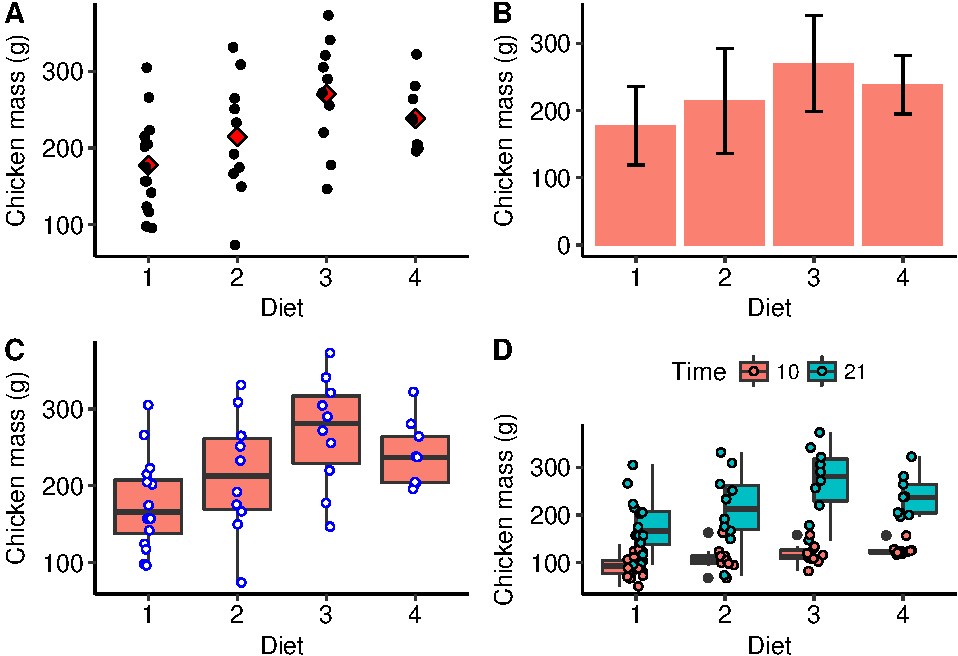
\includegraphics[width=0.7\linewidth]{03-discriptive_files/figure-latex/descriptive-plot1-1} \caption{A) Scatterplot of the mean and raw chicken mass values. B) Bar graph of the chicken mass values, showing whiskers indicating 1 ±SD. C) Box and whisker plot of the chicken mass data.}\label{fig:descriptive-plot1}
\end{figure}

\hypertarget{exercises}{%
\section{Exercises}\label{exercises}}

\hypertarget{exercise-1}{%
\subsection{Exercise 1}\label{exercise-1}}

Notice how the data summary for chicken weights contained within
\texttt{wt\_summary} is very similar to the summary returned for
\texttt{weight} when we apply \texttt{summary(chicks)}. Please use the
\texttt{summarise()} approach and construct a data summary with exactly
the same summary statistics for \texttt{weight} as that which
\texttt{summary()} returns.

\hypertarget{graphical-data-displays}{%
\chapter{Graphical data displays}\label{graphical-data-displays}}

\begin{Shaded}
\begin{Highlighting}[]
\KeywordTok{library}\NormalTok{(tidyverse)}
\KeywordTok{library}\NormalTok{(ggpubr)}
\KeywordTok{library}\NormalTok{(RColorBrewer)}
\KeywordTok{library}\NormalTok{(ggthemes)}
\end{Highlighting}
\end{Shaded}

Here we shall provide examples of many kinds of graphical data
summaries. We use \textbf{ggplot2} for these figures and will refrain
from using the base R graphs. We shall provide examples of various
themes so you can see what is available to use for your own plots. We
also include various modifications of the default plots so you can get
an idea of how to modify some of the plot characteristics, and we always
make sure that our graphs are publication ready. The best way to learn
is to work by example. Deeper understanding will emerge only from
working through all of these example plots, and making your own changes
here and there to see how your own modification will affect your graphs'
appearance. Then find your own data and plot them. As always, liberally
make use of the built-in help facility (the more you do, the easier it
becomes, like riding a bicycle). Also, don't be shy to use Google.

\hypertarget{qualitative-data-1}{%
\section{Qualitative data}\label{qualitative-data-1}}

Qualitative data that describe group representivity to various
categories are best presented as frequency distribution histograms (I
interchangeably use histograms, frequency histograms, and frequency
distribution histograms). Histograms apply to categorical data. Although
it can be presented numerically in tabular form, one more frequently
creates a bar or pie graph of the number of occurrences in a collection
of non-overlapping classes or categories. Both the data and graphical
displays will be demonstrated here.

The first case of a frequency distribution histogram is one that shows
the raw counts per each of the categories that are represented in the
data. The count within each of the categories (represented by a bar
graph called a histogram) sums to the sample size, \(n\). In the second
case, we may want to report those data as proportions. Here we show the
frequency proportion in a collection of non-overlapping categories. For
example, we have a sample size of 12 (\(n=12\)). In this sample, two are
coloured blue, six red, and five purple. The relative proportions are
\(2/12=0.1666667\) blue, \(6/12=0.5\) red, and \(5/12=0.4166667\)
purple. The important thing to note here is that the relative
proportions sum to 1, i.e. \(0.1666667+0.5+0.4166667=1\). These data may
be presented as a table or as a graph.

Let us demonstrate the numerical and graphical summaries using the
built-in \texttt{iris} data:

\begin{Shaded}
\begin{Highlighting}[]
\CommentTok{# the numerical summary produced by a piped series of functions;}
\CommentTok{# create a summary of the data (i.e. number of replicates per species)}
\CommentTok{# used for (A), (B) and (C), below}
\NormalTok{iris.cnt <-}\StringTok{ }\NormalTok{iris }\OperatorTok
\StringTok{  }\KeywordTok{count}\NormalTok{(Species) }\OperatorTok\StringTok{ }\CommentTok{# automagically creates a column, n, with the counts}
\StringTok{  }\KeywordTok{mutate}\NormalTok{(}\DataTypeTok{prop =}\NormalTok{ n }\OperatorTok{/}\StringTok{ }\KeywordTok{sum}\NormalTok{(n)) }\CommentTok{# creates the relative proportion of each species}
\NormalTok{iris.cnt}
\end{Highlighting}
\end{Shaded}

\begin{verbatim}
R> # A tibble: 3 x 3
R>   Species        n  prop
R>   <fct>      <int> <dbl>
R> 1 setosa        50 0.333
R> 2 versicolor    50 0.333
R> 3 virginica     50 0.333
\end{verbatim}

\begin{Shaded}
\begin{Highlighting}[]
\CommentTok{# a stacked bar graph with the cumulative sum of observations}
\NormalTok{plt1 <-}\StringTok{ }\KeywordTok{ggplot}\NormalTok{(}\DataTypeTok{data =}\NormalTok{ iris.cnt, }\KeywordTok{aes}\NormalTok{(}\DataTypeTok{x =} \StringTok{""}\NormalTok{, }\DataTypeTok{y =}\NormalTok{ n, }\DataTypeTok{fill =}\NormalTok{ Species)) }\OperatorTok{+}
\StringTok{  }\KeywordTok{geom_bar}\NormalTok{(}\DataTypeTok{width =} \DecValTok{1}\NormalTok{, }\DataTypeTok{stat =} \StringTok{"identity"}\NormalTok{) }\OperatorTok{+}
\StringTok{  }\KeywordTok{labs}\NormalTok{(}\DataTypeTok{title =} \StringTok{"Stacked bar graph"}\NormalTok{, }\DataTypeTok{subtitle =} \StringTok{"cumulative sum"}\NormalTok{,}
       \DataTypeTok{x =} \OtherTok{NULL}\NormalTok{, }\DataTypeTok{y =} \StringTok{"Count"}\NormalTok{) }\OperatorTok{+}
\StringTok{  }\KeywordTok{theme_pubclean}\NormalTok{() }\OperatorTok{+}\StringTok{ }\KeywordTok{scale_color_few}\NormalTok{() }\OperatorTok{+}
\StringTok{  }\KeywordTok{scale_fill_few}\NormalTok{()}

\CommentTok{# a stacked bar graph with the relative proportions of observations}
\NormalTok{plt2 <-}\StringTok{ }\KeywordTok{ggplot}\NormalTok{(}\DataTypeTok{data =}\NormalTok{ iris.cnt, }\KeywordTok{aes}\NormalTok{(}\DataTypeTok{x =} \StringTok{""}\NormalTok{, }\DataTypeTok{y =}\NormalTok{ prop, }\DataTypeTok{fill =}\NormalTok{ Species)) }\OperatorTok{+}
\StringTok{  }\KeywordTok{geom_bar}\NormalTok{(}\DataTypeTok{width =} \DecValTok{1}\NormalTok{, }\DataTypeTok{stat =} \StringTok{"identity"}\NormalTok{) }\OperatorTok{+}
\StringTok{  }\KeywordTok{scale_y_continuous}\NormalTok{(}\DataTypeTok{breaks =} \KeywordTok{c}\NormalTok{(}\FloatTok{0.00}\NormalTok{, }\FloatTok{0.33}\NormalTok{, }\FloatTok{0.66}\NormalTok{, }\FloatTok{1.00}\NormalTok{)) }\OperatorTok{+}
\StringTok{  }\KeywordTok{labs}\NormalTok{(}\DataTypeTok{title =} \StringTok{"Stacked bar graph"}\NormalTok{, }\DataTypeTok{subtitle =} \StringTok{"relative proportions"}\NormalTok{,}
       \DataTypeTok{x =} \OtherTok{NULL}\NormalTok{, }\DataTypeTok{y =} \StringTok{"Proportion"}\NormalTok{) }\OperatorTok{+}
\StringTok{  }\KeywordTok{theme_pubclean}\NormalTok{() }\OperatorTok{+}\StringTok{ }\KeywordTok{scale_color_few}\NormalTok{() }\OperatorTok{+}
\StringTok{  }\KeywordTok{scale_fill_few}\NormalTok{()}


\CommentTok{# a basic pie chart}
\NormalTok{plt3 <-}\StringTok{ }\NormalTok{plt1 }\OperatorTok{+}\StringTok{ }\KeywordTok{coord_polar}\NormalTok{(}\StringTok{"y"}\NormalTok{, }\DataTypeTok{start =} \DecValTok{0}\NormalTok{) }\OperatorTok{+}
\StringTok{  }\KeywordTok{labs}\NormalTok{(}\DataTypeTok{title =} \StringTok{"Friends don't let..."}\NormalTok{, }\DataTypeTok{subtitle =} \StringTok{"...friends make pie charts"}\NormalTok{,}
       \DataTypeTok{x =} \OtherTok{NULL}\NormalTok{, }\DataTypeTok{y =} \OtherTok{NULL}\NormalTok{) }\OperatorTok{+}
\StringTok{  }\KeywordTok{scale_fill_brewer}\NormalTok{(}\DataTypeTok{palette =} \StringTok{"Blues"}\NormalTok{) }\OperatorTok{+}
\StringTok{  }\KeywordTok{theme_minimal}\NormalTok{()}
\CommentTok{# if you seriously want a pie chart, rather use the base R function, `pie()`}

\CommentTok{# here now a bar graph...}
\CommentTok{# the default mapping of `geom_bar` is `stat = count`, which is a}
\CommentTok{# bar for each fo the categories (`Species`), with `count` along y}
\NormalTok{plt4 <-}\StringTok{ }\KeywordTok{ggplot}\NormalTok{(}\DataTypeTok{data =}\NormalTok{ iris, }\KeywordTok{aes}\NormalTok{(}\DataTypeTok{x =}\NormalTok{ Species, }\DataTypeTok{fill =}\NormalTok{ Species)) }\OperatorTok{+}
\StringTok{  }\KeywordTok{geom_bar}\NormalTok{(}\DataTypeTok{show.legend =} \OtherTok{FALSE}\NormalTok{) }\OperatorTok{+}
\StringTok{  }\KeywordTok{labs}\NormalTok{(}\DataTypeTok{title =} \StringTok{"Side-by-side bars"}\NormalTok{, }\DataTypeTok{subtitle =} \StringTok{"n per species"}\NormalTok{, }\DataTypeTok{y =} \StringTok{"Count"}\NormalTok{) }\OperatorTok{+}
\StringTok{ }\KeywordTok{theme_pubclean}\NormalTok{() }\OperatorTok{+}\StringTok{ }\KeywordTok{scale_color_few}\NormalTok{() }\OperatorTok{+}
\StringTok{  }\KeywordTok{scale_fill_few}\NormalTok{()}

\KeywordTok{ggarrange}\NormalTok{(plt1, plt2, plt3, plt4, }\DataTypeTok{nrow =} \DecValTok{2}\NormalTok{, }\DataTypeTok{ncol =} \DecValTok{2}\NormalTok{, }\DataTypeTok{labels =} \StringTok{"AUTO"}\NormalTok{)}
\end{Highlighting}
\end{Shaded}

\begin{figure}
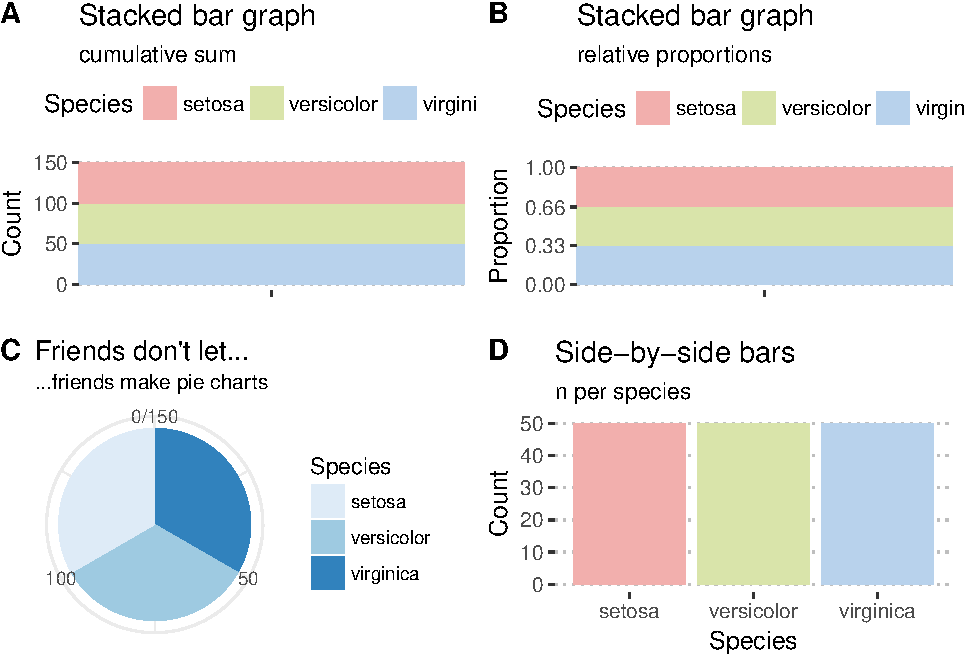
\includegraphics[width=0.7\linewidth]{04-graphics_files/figure-latex/graphics-plot1-1} \caption{Examples of histograms for the built-in Iris data. A) A default frequency histogram showing the count of samples for each of the three species. B) A relative frequency histogram of the same data; here, the sum of counts of samples available for each of the three species is 1. C) A boring pie chart. D) A frequency histogram of raw data counts shown as a series of side-by-side bars.}\label{fig:graphics-plot1}
\end{figure}

\hypertarget{continuous-data-1}{%
\section{Continuous data}\label{continuous-data-1}}

\hypertarget{frequency-distributions-histograms}{%
\subsection{Frequency distributions
(histograms)}\label{frequency-distributions-histograms}}

As with discrete data, we have a choice of absolute (Fig. 4.2A) and
relative (Fig. 4.2 B-C) frequency histograms. There's also the empirical
cumulative distribution function (ECDF) (Fig. 4.2 D) that uses relative
proportions, but in this instance it is the relative proportion that
each individual observation has towards the sample. Since the purpose of
frequency histograms is to count the number of times something takes
place or occurs within a category, what do we do when we are faced with
continuous data where no categories are available? We can create our own
categories, called \emph{bins}. See the Old Faithful data, for example.
The eruptions last between 1.6 and 5.1 minutes. So, we create intervals
of time spanning these times, and within each count the number of times
an event lasts as long as denoted by the intervals. Here we might choose
intervals of 1-2 minutes, 2-3 minutes, 3-4 minutes, 4-5 minutes, and 5-6
minutes. The \textbf{ggplot2} \texttt{geom\_histogram()} function
automatically creates the bins, but we may specify our own. It is best
to explain these principles by example (see Figure 4.2 A-D).

\begin{Shaded}
\begin{Highlighting}[]
\CommentTok{# a normal frequency histogram, with count along y}
\NormalTok{hist1 <-}\StringTok{ }\KeywordTok{ggplot}\NormalTok{(}\DataTypeTok{data =}\NormalTok{ faithful, }\KeywordTok{aes}\NormalTok{(}\DataTypeTok{x =}\NormalTok{ eruptions)) }\OperatorTok{+}
\StringTok{  }\KeywordTok{geom_histogram}\NormalTok{(}\DataTypeTok{colour =} \StringTok{"black"}\NormalTok{, }\DataTypeTok{fill =} \StringTok{"salmon"}\NormalTok{, }\DataTypeTok{alpha =} \FloatTok{0.6}\NormalTok{) }\OperatorTok{+}
\StringTok{  }\KeywordTok{labs}\NormalTok{(}\DataTypeTok{title =} \StringTok{"Old Faithful data"}\NormalTok{,}
       \DataTypeTok{subtitle =} \StringTok{"A vanilla frequency histogram"}\NormalTok{,}
       \DataTypeTok{x =} \StringTok{"Eruption duration (min)"}\NormalTok{,}
       \DataTypeTok{y =} \StringTok{"Count"}\NormalTok{) }\OperatorTok{+}\StringTok{ }\KeywordTok{theme_pubclean}\NormalTok{()}

\CommentTok{# when the binwidth is 1, the density histogram *is* the relative}
\CommentTok{# frequency histogram}
\NormalTok{hist2 <-}\StringTok{ }\KeywordTok{ggplot}\NormalTok{(}\DataTypeTok{data =}\NormalTok{ faithful, }\KeywordTok{aes}\NormalTok{(}\DataTypeTok{x =}\NormalTok{ eruptions)) }\OperatorTok{+}
\StringTok{  }\KeywordTok{geom_histogram}\NormalTok{(}\KeywordTok{aes}\NormalTok{(}\DataTypeTok{y =}\NormalTok{ ..density..),}
                 \DataTypeTok{position =} \StringTok{'identity'}\NormalTok{, }\DataTypeTok{binwidth =} \DecValTok{1}\NormalTok{,}
                 \DataTypeTok{colour =} \StringTok{"black"}\NormalTok{, }\DataTypeTok{fill =} \StringTok{"salmon"}\NormalTok{, }\DataTypeTok{alpha =} \FloatTok{0.6}\NormalTok{) }\OperatorTok{+}
\StringTok{  }\KeywordTok{labs}\NormalTok{(}\DataTypeTok{title =} \StringTok{"Old Faithful data"}\NormalTok{,}
       \DataTypeTok{subtitle =} \StringTok{"Relative frequency histogram"}\NormalTok{,}
       \DataTypeTok{x =} \StringTok{"Eruption duration (min)"}\NormalTok{,}
       \DataTypeTok{y =} \StringTok{"Count"}\NormalTok{) }\OperatorTok{+}\StringTok{ }\KeywordTok{theme_pubclean}\NormalTok{()}


\CommentTok{# if binwidth is something other than 1, the relative frequency in}
\CommentTok{# a histogram is ..density.. * binwidth}
\NormalTok{hist3 <-}\StringTok{ }\KeywordTok{ggplot}\NormalTok{(}\DataTypeTok{data =}\NormalTok{ faithful, }\KeywordTok{aes}\NormalTok{(}\DataTypeTok{x =}\NormalTok{ eruptions)) }\OperatorTok{+}
\StringTok{  }\KeywordTok{geom_histogram}\NormalTok{(}\KeywordTok{aes}\NormalTok{(}\DataTypeTok{y =} \FloatTok{0.5} \OperatorTok{*}\StringTok{ }\NormalTok{..density..),}
                 \DataTypeTok{position =} \StringTok{'identity'}\NormalTok{, }\DataTypeTok{binwidth =} \FloatTok{0.5}\NormalTok{,}
                 \DataTypeTok{colour =} \StringTok{"black"}\NormalTok{, }\DataTypeTok{fill =} \StringTok{"salmon"}\NormalTok{, }\DataTypeTok{alpha =} \FloatTok{0.6}\NormalTok{) }\OperatorTok{+}
\StringTok{  }\KeywordTok{labs}\NormalTok{(}\DataTypeTok{title =} \StringTok{"Old Faithful data"}\NormalTok{,}
       \DataTypeTok{subtitle =} \StringTok{"Relative frequency histogram"}\NormalTok{,}
       \DataTypeTok{x =} \StringTok{"Eruption duration (min)"}\NormalTok{,}
       \DataTypeTok{y =} \StringTok{"Relative contribution"}\NormalTok{) }\OperatorTok{+}\StringTok{ }\KeywordTok{theme_pubclean}\NormalTok{()}

\CommentTok{# ECDF}
\NormalTok{hist4 <-}\StringTok{ }\KeywordTok{ggplot}\NormalTok{(}\DataTypeTok{data =}\NormalTok{ faithful, }\KeywordTok{aes}\NormalTok{(}\DataTypeTok{x =}\NormalTok{ eruptions)) }\OperatorTok{+}\StringTok{ }
\StringTok{  }\KeywordTok{stat_ecdf}\NormalTok{() }\OperatorTok{+}
\StringTok{  }\KeywordTok{labs}\NormalTok{(}\DataTypeTok{title =} \StringTok{"Old Faithful data"}\NormalTok{,}
       \DataTypeTok{subtitle =} \StringTok{"ECDF"}\NormalTok{,}
       \DataTypeTok{x =} \StringTok{"Eruption duration (min)"}\NormalTok{,}
       \DataTypeTok{y =} \StringTok{"Relative contribution"}\NormalTok{) }\OperatorTok{+}\StringTok{ }\KeywordTok{theme_pubclean}\NormalTok{()}

\KeywordTok{ggarrange}\NormalTok{(hist1, hist2, hist3, hist4, }\DataTypeTok{ncol =} \DecValTok{2}\NormalTok{, }\DataTypeTok{nrow =} \DecValTok{2}\NormalTok{, }\DataTypeTok{labels =} \StringTok{"AUTO"}\NormalTok{)}
\end{Highlighting}
\end{Shaded}

\begin{figure}
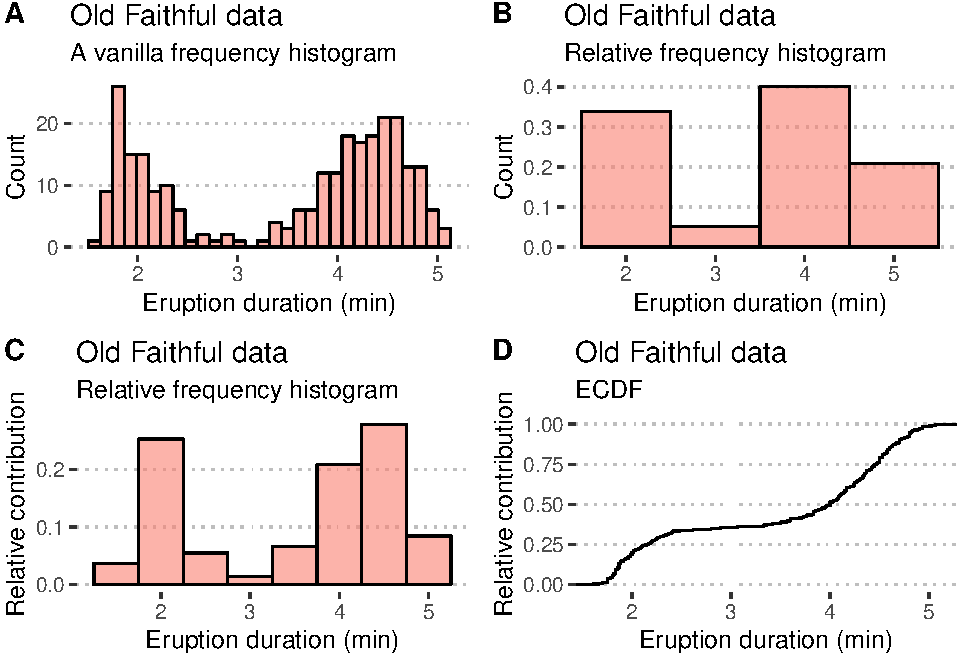
\includegraphics[width=0.7\linewidth]{04-graphics_files/figure-latex/graphics-plot2-1} \caption{Example histograms for the Old Faithful data. A) A default frequency histogram with the count of eruption times falling within the specified bins. B) A relative frequency histogram with bins adjusted to a width of 1 minute intervals; here, the sum of counts within each of the four bins is 1. C) Another relative frequency histogram, but with the bins adjusted to each be 0.5 minute increments; again the sum of counts represented by each bin is equal to 1.}\label{fig:graphics-plot2}
\end{figure}

What if we have continuous data belonging with multiple categories? The
\texttt{iris} data provide a nice set of measurements that we may use to
demonstrate a grouped frequency histogram. These data are size
measurements (cm) of the variables sepal length and width and petal
length and width, respectively, for 50 flowers from each of three
species of \emph{Iris}. The species are \emph{Iris setosa}, \emph{I.
versicolor}, and \emph{I. virginica}.

\begin{Shaded}
\begin{Highlighting}[]
\CommentTok{# first we make long data}
\NormalTok{iris.long <-}\StringTok{ }\NormalTok{iris }\OperatorTok\StringTok{ }
\StringTok{  }\KeywordTok{gather}\NormalTok{(}\DataTypeTok{key =} \StringTok{"variable"}\NormalTok{, }\DataTypeTok{value =} \StringTok{"size"}\NormalTok{, }\OperatorTok{-}\NormalTok{Species)}

\KeywordTok{ggplot}\NormalTok{(}\DataTypeTok{data =}\NormalTok{ iris.long, }\KeywordTok{aes}\NormalTok{(}\DataTypeTok{x =}\NormalTok{ size)) }\OperatorTok{+}
\StringTok{  }\KeywordTok{geom_histogram}\NormalTok{(}\DataTypeTok{position =} \StringTok{"dodge"}\NormalTok{, }\CommentTok{# ommitting this creates a stacked histogram}
                 \DataTypeTok{colour =} \OtherTok{NA}\NormalTok{, }\DataTypeTok{bins =} \DecValTok{20}\NormalTok{,}
                 \KeywordTok{aes}\NormalTok{(}\DataTypeTok{fill =}\NormalTok{ Species)) }\OperatorTok{+}
\StringTok{  }\KeywordTok{facet_wrap}\NormalTok{(}\OperatorTok{~}\NormalTok{variable) }\OperatorTok{+}
\StringTok{  }\KeywordTok{labs}\NormalTok{(}\DataTypeTok{title =} \StringTok{"Iris data"}\NormalTok{,}
       \DataTypeTok{subtitle =} \StringTok{"Grouped frequency histogram"}\NormalTok{,}
       \DataTypeTok{x =} \StringTok{"Size (mm)"}\NormalTok{,}
       \DataTypeTok{y =} \StringTok{"Count"}\NormalTok{) }\OperatorTok{+}
\StringTok{  }\KeywordTok{theme_pubclean}\NormalTok{()}
\end{Highlighting}
\end{Shaded}

\begin{figure}
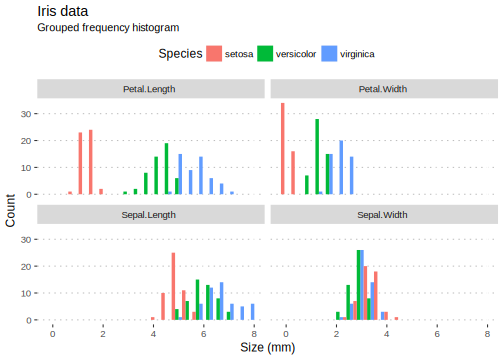
\includegraphics[width=0.7\linewidth]{04-graphics_files/figure-latex/graphics-plot3-1} \caption{Panelled grouped histograms for the four Iris variables.}\label{fig:graphics-plot3}
\end{figure}

\hypertarget{box-plots}{%
\subsection{Box plots}\label{box-plots}}

Box plots are sometimes called box-and-whisker plots. These graphs are a
a graphical representation of the data based on its quartiles as well as
its smallest and largest values. The keen eye can glance the
\enquote{shape} of the data distribution; they provide an alternative
view to that given by the frequency distribution. A variation of the
basic box-and-whisker plot is to superimpose a jittered scatter plot of
the raw data on each bar.

From the \texttt{geom\_boxplot} documentation, which says it best (type
\texttt{?geom\_boxplot}):

\enquote{The lower and upper hinges correspond to the first and third
quartiles (the 25th and 75th percentiles).}

\enquote{The upper whisker extends from the hinge to the largest value
no further than 1.5 * IQR from the hinge (where IQR is the
inter-quartile range, or distance between the first and third
quartiles). The lower whisker extends from the hinge to the smallest
value at most 1.5 * IQR of the hinge. Data beyond the end of the
whiskers are called \enquote{outlying} points and are plotted
individually.}

\enquote{In a notched box plot, the notches extend 1.58 * IQR / sqrt(n).
This gives a roughly 95\% confidence interval for comparing medians.}

Here be examples:

\begin{Shaded}
\begin{Highlighting}[]
\NormalTok{plt1 <-}\StringTok{ }\KeywordTok{ggplot}\NormalTok{(}\DataTypeTok{data =}\NormalTok{ iris, }\KeywordTok{aes}\NormalTok{(}\DataTypeTok{x =}\NormalTok{ Species, }\DataTypeTok{y =}\NormalTok{ Sepal.Length, }\DataTypeTok{fill =}\NormalTok{ Species)) }\OperatorTok{+}
\StringTok{  }\KeywordTok{geom_boxplot}\NormalTok{(}\DataTypeTok{show.legend =} \OtherTok{FALSE}\NormalTok{, }\DataTypeTok{notch =} \OtherTok{FALSE}\NormalTok{) }\OperatorTok{+}\StringTok{ }\KeywordTok{theme_pubclean}\NormalTok{() }\OperatorTok{+}
\StringTok{  }\KeywordTok{labs}\NormalTok{(}\DataTypeTok{y =} \StringTok{"Sepal length (mm)"}\NormalTok{) }\OperatorTok{+}
\StringTok{  }\KeywordTok{theme}\NormalTok{(}\DataTypeTok{axis.text.x =} \KeywordTok{element_text}\NormalTok{(}\DataTypeTok{face =} \StringTok{"italic"}\NormalTok{))}

\NormalTok{plt2 <-}\StringTok{ }\KeywordTok{ggplot}\NormalTok{(}\DataTypeTok{data =}\NormalTok{ iris.long, }\KeywordTok{aes}\NormalTok{(}\DataTypeTok{x =}\NormalTok{ Species, }\DataTypeTok{y =}\NormalTok{ size)) }\OperatorTok{+}
\StringTok{  }\KeywordTok{geom_boxplot}\NormalTok{(}\DataTypeTok{fill =} \StringTok{"red"}\NormalTok{, }\DataTypeTok{alpha =} \FloatTok{0.4}\NormalTok{, }\DataTypeTok{notch =} \OtherTok{TRUE}\NormalTok{) }\OperatorTok{+}
\StringTok{  }\KeywordTok{geom_jitter}\NormalTok{(}\DataTypeTok{width =} \FloatTok{0.1}\NormalTok{, }\DataTypeTok{shape =} \DecValTok{21}\NormalTok{, }\DataTypeTok{colour =} \StringTok{"blue"}\NormalTok{, }\DataTypeTok{fill =} \OtherTok{NA}\NormalTok{, }\DataTypeTok{alpha =} \FloatTok{0.2}\NormalTok{) }\OperatorTok{+}
\StringTok{  }\KeywordTok{facet_wrap}\NormalTok{(}\OperatorTok{~}\NormalTok{variable, }\DataTypeTok{nrow =} \DecValTok{1}\NormalTok{) }\OperatorTok{+}
\StringTok{  }\KeywordTok{labs}\NormalTok{(}\DataTypeTok{y =} \StringTok{"Size (mm)"}\NormalTok{) }\OperatorTok{+}\StringTok{ }\KeywordTok{theme_pubclean}\NormalTok{() }\OperatorTok{+}
\StringTok{  }\KeywordTok{theme}\NormalTok{(}\DataTypeTok{axis.text.x =} \KeywordTok{element_text}\NormalTok{(}\DataTypeTok{face =} \StringTok{"italic"}\NormalTok{)) }\OperatorTok{+}
\StringTok{  }\KeywordTok{theme}\NormalTok{(}\DataTypeTok{axis.ticks.length=}\KeywordTok{unit}\NormalTok{(}\OperatorTok{-}\FloatTok{0.25}\NormalTok{, }\StringTok{"cm"}\NormalTok{), }\DataTypeTok{axis.ticks.margin=}\KeywordTok{unit}\NormalTok{(}\FloatTok{0.5}\NormalTok{, }\StringTok{"cm"}\NormalTok{))}

\KeywordTok{ggarrange}\NormalTok{(plt1, plt2, }\DataTypeTok{nrow =} \DecValTok{2}\NormalTok{, }\DataTypeTok{ncol =} \DecValTok{1}\NormalTok{, }\DataTypeTok{labels =} \StringTok{"AUTO"}\NormalTok{)}
\end{Highlighting}
\end{Shaded}

\begin{figure}
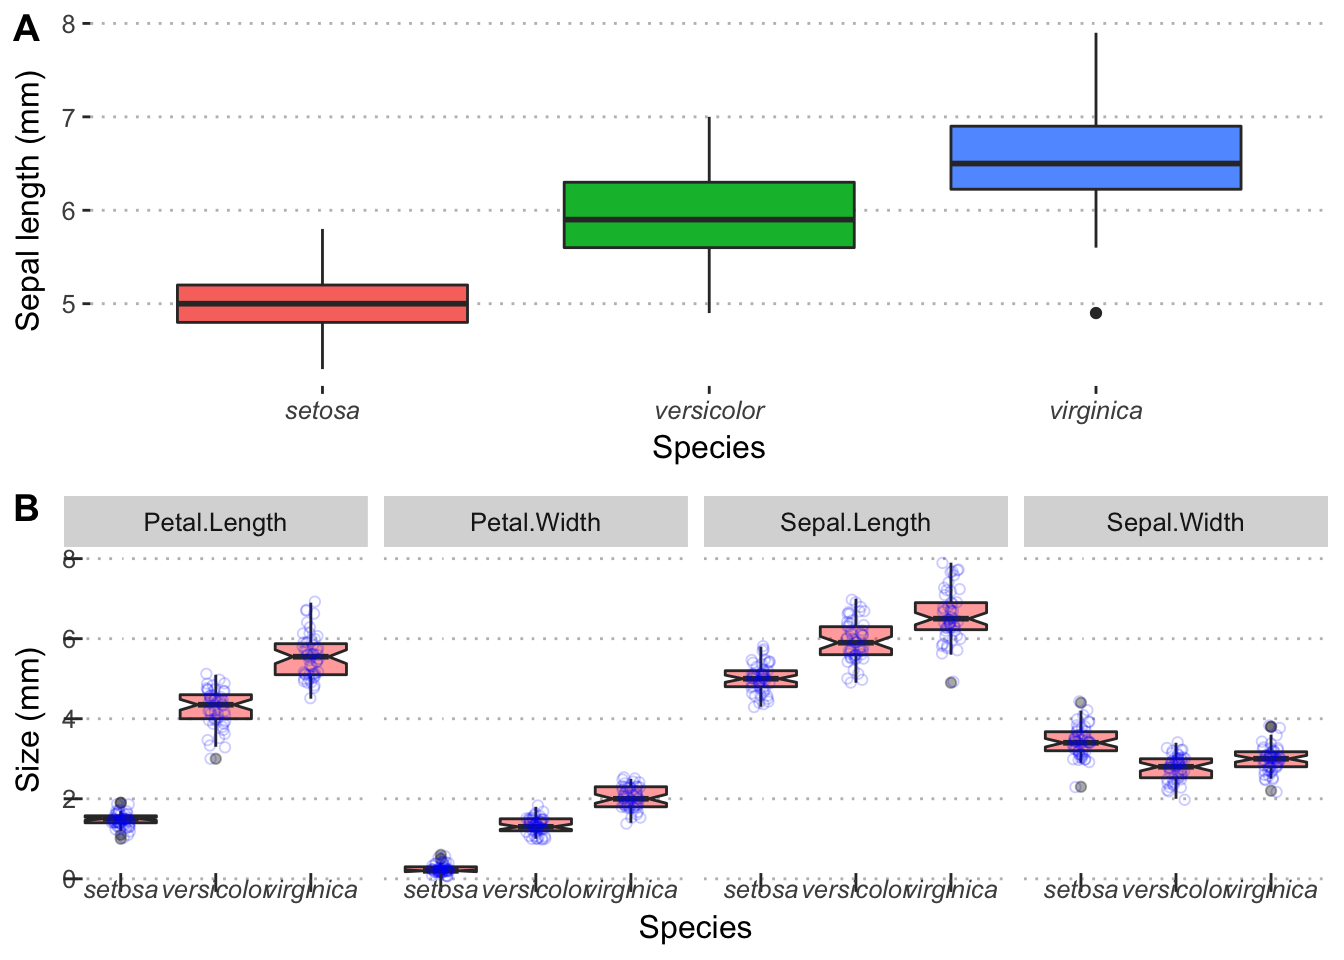
\includegraphics[width=0.7\linewidth]{04-graphics_files/figure-latex/graphics-plot4-1} \caption{Examples of box plots made for the Iris data. A) A default box plot for one of the variables only. B) A panelled collection of box plots, one for each of the four variables, with a scatterplot to indicate the spread of the actual replicates.}\label{fig:graphics-plot4}
\end{figure}

Box-and-whisker plots have traditionally been used to display data that
are not normally distributed, but I like to use them for any old data,
even normal data. I prefer these over the old-fashioned bar graphs (as
seen later in this section).

The \textbf{ggpubr} package provides many convenience functions for the
drawing of publication quality graphs, many of which include summaries
of pairwise comparisons (e.g.~in t-tests and ANOVAs). Please see
\href{http://www.sthda.com/english/articles/24-ggpubr-publication-ready-plots/}{here}
and \href{http://www.sthda.com/english/rpkgs/ggpubr/}{here}.

\hypertarget{pairwise-scatter-plots}{%
\subsection{Pairwise Scatter plots}\label{pairwise-scatter-plots}}

This graph shows the relationship between two (matched) continuous
variables. The statistical strength of the relationship can be indicated
by a correlation (no causal relationship implied as is the case here) or
a regression (when a causal link of \(x\) on \(y\) is demonstrated).

\begin{Shaded}
\begin{Highlighting}[]
\NormalTok{plt1 <-}\StringTok{ }\KeywordTok{ggplot}\NormalTok{(}\DataTypeTok{data =}\NormalTok{ iris, }\KeywordTok{aes}\NormalTok{(}\DataTypeTok{x =}\NormalTok{ Petal.Length, }\DataTypeTok{y =}\NormalTok{ Petal.Width, }\DataTypeTok{colour =}\NormalTok{ Species)) }\OperatorTok{+}
\StringTok{  }\KeywordTok{geom_point}\NormalTok{() }\OperatorTok{+}
\StringTok{  }\KeywordTok{labs}\NormalTok{(}\DataTypeTok{x =} \StringTok{"Petal length (mm)"}\NormalTok{, }\DataTypeTok{y =} \StringTok{"Petal width (mm)"}\NormalTok{) }\OperatorTok{+}
\StringTok{  }\KeywordTok{theme}\NormalTok{(}\DataTypeTok{legend.position =} \KeywordTok{c}\NormalTok{(}\FloatTok{0.18}\NormalTok{, }\FloatTok{0.85}\NormalTok{)) }\OperatorTok{+}
\StringTok{  }\KeywordTok{scale_color_fivethirtyeight}\NormalTok{() }\OperatorTok{+}
\StringTok{  }\KeywordTok{scale_fill_fivethirtyeight}\NormalTok{() }\OperatorTok{+}\StringTok{ }
\StringTok{  }\KeywordTok{theme_pubclean}\NormalTok{()}

\NormalTok{plt2 <-}\StringTok{ }\KeywordTok{ggplot}\NormalTok{(}\DataTypeTok{data =}\NormalTok{ iris, }\KeywordTok{aes}\NormalTok{(}\DataTypeTok{x =}\NormalTok{ Petal.Length, }\DataTypeTok{y =}\NormalTok{ Petal.Width, }\DataTypeTok{colour =}\NormalTok{ Species)) }\OperatorTok{+}
\StringTok{  }\KeywordTok{geom_point}\NormalTok{(}\DataTypeTok{show.legend =} \OtherTok{FALSE}\NormalTok{) }\OperatorTok{+}
\StringTok{  }\KeywordTok{geom_smooth}\NormalTok{(}\DataTypeTok{method =} \StringTok{"lm"}\NormalTok{, }\DataTypeTok{se =} \OtherTok{FALSE}\NormalTok{, }\DataTypeTok{show.legend =} \OtherTok{FALSE}\NormalTok{) }\OperatorTok{+}
\StringTok{  }\KeywordTok{scale_color_fivethirtyeight}\NormalTok{() }\OperatorTok{+}
\StringTok{  }\KeywordTok{scale_fill_fivethirtyeight}\NormalTok{() }\OperatorTok{+}
\StringTok{  }\KeywordTok{labs}\NormalTok{(}\DataTypeTok{x =} \StringTok{"Petal length (mm)"}\NormalTok{, }\DataTypeTok{y =} \StringTok{"Petal width (mm)"}\NormalTok{) }\OperatorTok{+}\StringTok{ }
\StringTok{  }\KeywordTok{theme_pubclean}\NormalTok{()}

\KeywordTok{ggarrange}\NormalTok{(plt1, plt2, }\DataTypeTok{ncol =} \DecValTok{2}\NormalTok{, }\DataTypeTok{nrow =} \DecValTok{1}\NormalTok{, }\DataTypeTok{labels =} \StringTok{"AUTO"}\NormalTok{)}
\end{Highlighting}
\end{Shaded}

\begin{figure}
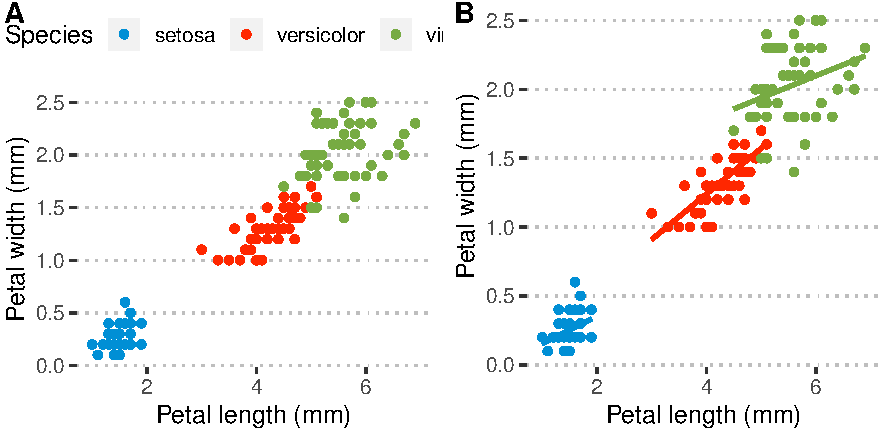
\includegraphics[width=0.7\linewidth]{04-graphics_files/figure-latex/graphics-plot5-1} \caption{Examples of scatterplots made for the Iris data. A) A default scatter plot showing the relationship between petal length and width. B) The same as (A) but with a correlation line added.}\label{fig:graphics-plot5}
\end{figure}

\hypertarget{bar-graphs}{%
\subsection{Bar graphs}\label{bar-graphs}}

Bar graphs display the mean plus/minus some measure of variation around
the mean---typically the standard error or the standard deviation. The
mean±SE and mean±SD are typically used for normally-distributed data.
Here I provide an example bar graph for one of the Iris data set's
variables:

\begin{Shaded}
\begin{Highlighting}[]
\CommentTok{# first make nice labels for the facets because the default ones}
\CommentTok{# in the dataframe are not so nice; use the `labeller()` function}
\CommentTok{# to receive the new variable names defined here}
\NormalTok{facet.names <-}\StringTok{ }\KeywordTok{c}\NormalTok{(}\DataTypeTok{Petal.Length =} \StringTok{"Petal length"}\NormalTok{,}
                 \DataTypeTok{Petal.Width =} \StringTok{"Petal width"}\NormalTok{,}
                 \DataTypeTok{Sepal.Length =} \StringTok{"Sepal length"}\NormalTok{,}
                 \DataTypeTok{Sepal.Width =} \StringTok{"Sepal width"}\NormalTok{)}

\CommentTok{# start with the `iris.long` long data that were produced above}
\CommentTok{# we create summaries of mean and SD and squirt it directly}
\CommentTok{# into the ggplot functions}
\NormalTok{iris.long }\OperatorTok\StringTok{ }
\StringTok{  }\KeywordTok{group_by}\NormalTok{(Species, variable) }\OperatorTok
\StringTok{  }\KeywordTok{summarise}\NormalTok{(}\DataTypeTok{mean.size =} \KeywordTok{mean}\NormalTok{(size),}
            \DataTypeTok{sd.size =} \KeywordTok{sd}\NormalTok{(size)) }\OperatorTok
\StringTok{  }\KeywordTok{ggplot}\NormalTok{(}\KeywordTok{aes}\NormalTok{(}\DataTypeTok{x =}\NormalTok{ Species, }\DataTypeTok{y =}\NormalTok{ mean.size)) }\OperatorTok{+}
\StringTok{  }\KeywordTok{geom_bar}\NormalTok{(}\DataTypeTok{stat =} \StringTok{"identity"}\NormalTok{) }\OperatorTok{+}
\StringTok{  }\KeywordTok{geom_errorbar}\NormalTok{(}\KeywordTok{aes}\NormalTok{(}\DataTypeTok{ymin =}\NormalTok{ mean.size }\OperatorTok{-}\StringTok{ }\NormalTok{sd.size, }\DataTypeTok{ymax =}\NormalTok{ mean.size }\OperatorTok{+}\StringTok{ }\NormalTok{sd.size), }\DataTypeTok{width =} \FloatTok{0.2}\NormalTok{) }\OperatorTok{+}
\StringTok{  }\KeywordTok{facet_wrap}\NormalTok{(}\OperatorTok{~}\NormalTok{variable, }\DataTypeTok{labeller =} \KeywordTok{labeller}\NormalTok{(}\DataTypeTok{variable =}\NormalTok{ facet.names)) }\OperatorTok{+}
\StringTok{  }\KeywordTok{labs}\NormalTok{(}\DataTypeTok{y =} \StringTok{"Size (mm)"}\NormalTok{, }\DataTypeTok{title =} \StringTok{"A box plot..."}\NormalTok{, }\DataTypeTok{subtitle =} \StringTok{"...of the Iris data"}\NormalTok{) }\OperatorTok{+}
\StringTok{  }\KeywordTok{theme}\NormalTok{(}\DataTypeTok{axis.text.x =} \KeywordTok{element_text}\NormalTok{(}\DataTypeTok{face =} \StringTok{"italic"}\NormalTok{))}
\end{Highlighting}
\end{Shaded}

\begin{figure}
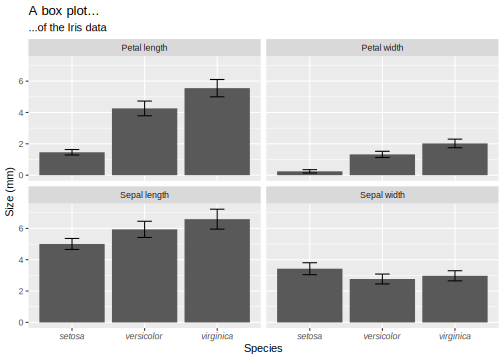
\includegraphics[width=0.7\linewidth]{04-graphics_files/figure-latex/graphics-plot6-1} \caption{Box plots of the mean ± SD of the four Iris variables.}\label{fig:graphics-plot6}
\end{figure}

\hypertarget{density-graphs}{%
\subsection{Density graphs}\label{density-graphs}}

Often when we are displaying a distribution of data we are interested in
the \enquote{shape} of the data more than the actual count of values in
a specific category, as shown by a standard histogram. When one wishes
to more organically visualise the frequency of values in a sample set a
density graphs is used. These may also be thought of as smooth
histograms. These work well with histograms and rug plots, as we may see
in the figure below. It is important to note with density plots that
they show the relative density of the distribution along the Y axis, and
\emph{not} the counts of the data. This can of course be changed, as
seen below, but is not the default setting. Sometimes it can be
informative to see how different the count and density distributions
appear.

\begin{Shaded}
\begin{Highlighting}[]
\CommentTok{# a normal density graph}
\NormalTok{dens1 <-}\StringTok{ }\KeywordTok{ggplot}\NormalTok{(}\DataTypeTok{data =}\NormalTok{ faithful, }\KeywordTok{aes}\NormalTok{(}\DataTypeTok{x =}\NormalTok{ eruptions)) }\OperatorTok{+}
\StringTok{  }\KeywordTok{geom_density}\NormalTok{(}\DataTypeTok{colour =} \StringTok{"black"}\NormalTok{, }\DataTypeTok{fill =} \StringTok{"salmon"}\NormalTok{, }\DataTypeTok{alpha =} \FloatTok{0.6}\NormalTok{) }\OperatorTok{+}
\StringTok{  }\KeywordTok{labs}\NormalTok{(}\DataTypeTok{title =} \StringTok{"Old Faithful data"}\NormalTok{,}
       \DataTypeTok{subtitle =} \StringTok{"A vanilla density plot"}\NormalTok{,}
       \DataTypeTok{x =} \StringTok{"Eruption duration (min)"}\NormalTok{,}
       \DataTypeTok{y =} \StringTok{"Density"}\NormalTok{) }\OperatorTok{+}\StringTok{ }\KeywordTok{theme_pubr}\NormalTok{()}

\CommentTok{# a density and rug plot combo}
\NormalTok{dens2 <-}\StringTok{ }\KeywordTok{ggplot}\NormalTok{(}\DataTypeTok{data =}\NormalTok{ faithful, }\KeywordTok{aes}\NormalTok{(}\DataTypeTok{x =}\NormalTok{ eruptions)) }\OperatorTok{+}
\StringTok{  }\KeywordTok{geom_density}\NormalTok{(}\DataTypeTok{colour =} \StringTok{"black"}\NormalTok{, }\DataTypeTok{fill =} \StringTok{"salmon"}\NormalTok{, }\DataTypeTok{alpha =} \FloatTok{0.6}\NormalTok{) }\OperatorTok{+}
\StringTok{  }\KeywordTok{geom_rug}\NormalTok{(}\DataTypeTok{colour =} \StringTok{"red"}\NormalTok{) }\OperatorTok{+}
\StringTok{  }\KeywordTok{labs}\NormalTok{(}\DataTypeTok{title =} \StringTok{"Old Faithful data"}\NormalTok{,}
       \DataTypeTok{subtitle =} \StringTok{"A density and rug plot"}\NormalTok{,}
       \DataTypeTok{x =} \StringTok{"Eruption duration (min)"}\NormalTok{,}
       \DataTypeTok{y =} \StringTok{"Density"}\NormalTok{) }\OperatorTok{+}\StringTok{ }\KeywordTok{theme_pubr}\NormalTok{()}

\CommentTok{# a relative frequency histogram overlayed with a density plot}
\NormalTok{dens3 <-}\StringTok{ }\KeywordTok{ggplot}\NormalTok{(}\DataTypeTok{data =}\NormalTok{ faithful, }\KeywordTok{aes}\NormalTok{(}\DataTypeTok{x =}\NormalTok{ eruptions)) }\OperatorTok{+}
\StringTok{  }\KeywordTok{geom_histogram}\NormalTok{(}\KeywordTok{aes}\NormalTok{(}\DataTypeTok{y =}\NormalTok{ ..density..),}
                 \DataTypeTok{position =} \StringTok{'identity'}\NormalTok{, }\DataTypeTok{binwidth =} \DecValTok{1}\NormalTok{,}
                 \DataTypeTok{colour =} \StringTok{"black"}\NormalTok{, }\DataTypeTok{fill =} \StringTok{"turquoise"}\NormalTok{, }\DataTypeTok{alpha =} \FloatTok{0.6}\NormalTok{) }\OperatorTok{+}
\StringTok{  }\KeywordTok{geom_density}\NormalTok{(}\DataTypeTok{colour =} \StringTok{"black"}\NormalTok{, }\DataTypeTok{fill =} \StringTok{"salmon"}\NormalTok{, }\DataTypeTok{alpha =} \FloatTok{0.6}\NormalTok{) }\OperatorTok{+}
\StringTok{  }\KeywordTok{labs}\NormalTok{(}\DataTypeTok{title =} \StringTok{"Old Faithful data"}\NormalTok{,}
       \DataTypeTok{subtitle =} \StringTok{"Relative frequency with density"}\NormalTok{,}
       \DataTypeTok{x =} \StringTok{"Eruption duration (min)"}\NormalTok{,}
       \DataTypeTok{y =} \StringTok{"Density"}\NormalTok{) }\OperatorTok{+}\StringTok{ }\KeywordTok{theme_pubr}\NormalTok{()}

\CommentTok{# a normal frequency histogram with density overlayed}
\CommentTok{# note that the density curve must be adjusted by}
\CommentTok{# the number of data points times the bin width}
\NormalTok{dens4 <-}\StringTok{ }\KeywordTok{ggplot}\NormalTok{(}\DataTypeTok{data =}\NormalTok{ faithful, }\KeywordTok{aes}\NormalTok{(}\DataTypeTok{x =}\NormalTok{ eruptions)) }\OperatorTok{+}
\StringTok{  }\KeywordTok{geom_histogram}\NormalTok{(}\KeywordTok{aes}\NormalTok{(}\DataTypeTok{y =}\NormalTok{ ..count..),}
                 \DataTypeTok{binwidth =} \FloatTok{0.2}\NormalTok{, }\DataTypeTok{colour =} \StringTok{"black"}\NormalTok{, }\DataTypeTok{fill =} \StringTok{"turquoise"}\NormalTok{, }\DataTypeTok{alpha =} \FloatTok{0.6}\NormalTok{) }\OperatorTok{+}
\StringTok{  }\KeywordTok{geom_density}\NormalTok{(}\KeywordTok{aes}\NormalTok{(}\DataTypeTok{y =}\NormalTok{ ..density.. }\OperatorTok{*}\StringTok{ }\KeywordTok{nrow}\NormalTok{(datasets}\OperatorTok{::}\NormalTok{faithful) }\OperatorTok{*}\StringTok{ }\FloatTok{0.2}\NormalTok{), }\DataTypeTok{position =} \StringTok{"identity"}\NormalTok{,}
               \DataTypeTok{colour =} \StringTok{"black"}\NormalTok{, }\DataTypeTok{fill =} \StringTok{"salmon"}\NormalTok{, }\DataTypeTok{alpha =} \FloatTok{0.6}\NormalTok{) }\OperatorTok{+}
\StringTok{  }\KeywordTok{labs}\NormalTok{(}\DataTypeTok{title =} \StringTok{"Old Faithful data"}\NormalTok{,}
       \DataTypeTok{subtitle =} \StringTok{"Frequency with density"}\NormalTok{,}
       \DataTypeTok{x =} \StringTok{"Eruption duration (min)"}\NormalTok{,}
       \DataTypeTok{y =} \StringTok{"Count"}\NormalTok{) }\OperatorTok{+}\StringTok{ }\KeywordTok{theme_pubr}\NormalTok{()}

\KeywordTok{ggarrange}\NormalTok{(dens1, dens2, dens3, dens4, }\DataTypeTok{ncol =} \DecValTok{2}\NormalTok{, }\DataTypeTok{nrow =} \DecValTok{2}\NormalTok{, }\DataTypeTok{labels =} \StringTok{"AUTO"}\NormalTok{)}
\end{Highlighting}
\end{Shaded}

\begin{figure}
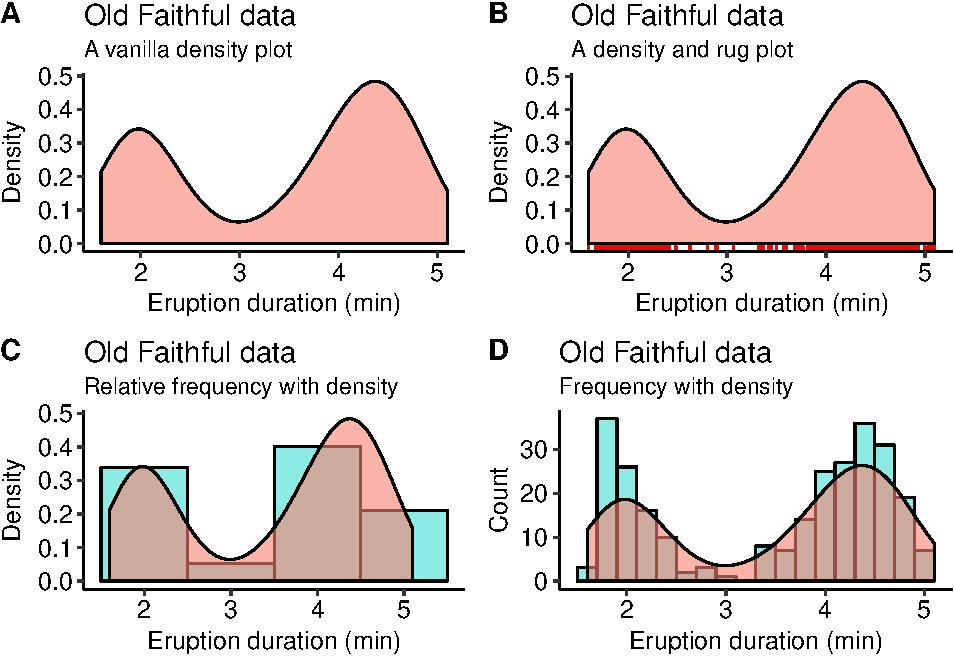
\includegraphics[width=0.7\linewidth]{04-graphics_files/figure-latex/graphics-plot7-1} \caption{A bevy of density graphs option based on the iris data. A) A lone density graph. B) A density graph accompanied by a rug plot. C) A histogram with a density graph overlay. D) A ridge plot.}\label{fig:graphics-plot7}
\end{figure}

\hypertarget{violin-plots}{%
\subsection{Violin plots}\label{violin-plots}}

The density graph is not limited to it's use with histograms. We may
combine this concept with box plots, too. These are known as violin
plots and are very useful when we want to show the distribution of
multiple categories of the same variable alongside one another. Violin
plots may show the same information as box plots but take things one
step further by allowing the shape of the boxplot to also show the
distribution of the data within the sample set. We will use the
\texttt{iris} data below to highlight the different types of violin
plots one may use.

\begin{Shaded}
\begin{Highlighting}[]
\CommentTok{# A basic violin plot}
\NormalTok{vio1 <-}\StringTok{ }\KeywordTok{ggplot}\NormalTok{(}\DataTypeTok{data =}\NormalTok{ iris, }\KeywordTok{aes}\NormalTok{(}\DataTypeTok{x =}\NormalTok{ Species, }\DataTypeTok{y =}\NormalTok{ Sepal.Length, }\DataTypeTok{fill =}\NormalTok{ Species)) }\OperatorTok{+}
\StringTok{  }\KeywordTok{geom_violin}\NormalTok{() }\OperatorTok{+}\StringTok{ }
\StringTok{  }\KeywordTok{theme_pubclean}\NormalTok{() }\OperatorTok{+}\StringTok{ }\KeywordTok{theme}\NormalTok{(}\DataTypeTok{legend.position =} \StringTok{"none"}\NormalTok{) }\OperatorTok{+}
\StringTok{  }\KeywordTok{labs}\NormalTok{(}\DataTypeTok{title =} \StringTok{"Iris data"}\NormalTok{,}
       \DataTypeTok{subtitle =} \StringTok{"Basic violin plot"}\NormalTok{, }\DataTypeTok{y =} \StringTok{"Sepal length (mm)"}\NormalTok{) }\OperatorTok{+}
\StringTok{  }\KeywordTok{theme}\NormalTok{(}\DataTypeTok{axis.text.x =} \KeywordTok{element_text}\NormalTok{(}\DataTypeTok{face =} \StringTok{"italic"}\NormalTok{))}

\CommentTok{# Aviolin plot showing the quartiles as lines}
\NormalTok{vio2 <-}\StringTok{ }\KeywordTok{ggplot}\NormalTok{(}\DataTypeTok{data =}\NormalTok{ iris, }\KeywordTok{aes}\NormalTok{(}\DataTypeTok{x =}\NormalTok{ Species, }\DataTypeTok{y =}\NormalTok{ Sepal.Length, }\DataTypeTok{fill =}\NormalTok{ Species)) }\OperatorTok{+}
\StringTok{  }\KeywordTok{geom_violin}\NormalTok{(}\DataTypeTok{show.legend =} \OtherTok{FALSE}\NormalTok{, }\DataTypeTok{draw_quantiles =} \KeywordTok{c}\NormalTok{(}\FloatTok{0.25}\NormalTok{, }\FloatTok{0.5}\NormalTok{, }\FloatTok{0.75}\NormalTok{)) }\OperatorTok{+}\StringTok{ }
\StringTok{  }\KeywordTok{theme_pubclean}\NormalTok{() }\OperatorTok{+}\StringTok{ }\KeywordTok{theme}\NormalTok{(}\DataTypeTok{legend.position =} \StringTok{"none"}\NormalTok{) }\OperatorTok{+}
\StringTok{  }\KeywordTok{labs}\NormalTok{(}\DataTypeTok{title =} \StringTok{"Iris data"}\NormalTok{,}
       \DataTypeTok{subtitle =} \StringTok{"Violin plot with quartiles"}\NormalTok{, }\DataTypeTok{y =} \StringTok{"Sepal length (mm)"}\NormalTok{) }\OperatorTok{+}
\StringTok{  }\KeywordTok{theme}\NormalTok{(}\DataTypeTok{axis.text.x =} \KeywordTok{element_text}\NormalTok{(}\DataTypeTok{face =} \StringTok{"italic"}\NormalTok{))}

\CommentTok{# Box plots nested within violin plots}
\NormalTok{vio3 <-}\StringTok{ }\KeywordTok{ggplot}\NormalTok{(}\DataTypeTok{data =}\NormalTok{ iris, }\KeywordTok{aes}\NormalTok{(}\DataTypeTok{x =}\NormalTok{ Species, }\DataTypeTok{y =}\NormalTok{ Sepal.Length, }\DataTypeTok{colour =}\NormalTok{ Species)) }\OperatorTok{+}
\StringTok{  }\KeywordTok{geom_violin}\NormalTok{(}\DataTypeTok{fill =} \StringTok{"grey70"}\NormalTok{) }\OperatorTok{+}\StringTok{ }
\StringTok{  }\KeywordTok{geom_boxplot}\NormalTok{(}\DataTypeTok{width =} \FloatTok{0.1}\NormalTok{, }\DataTypeTok{colour =} \StringTok{"grey30"}\NormalTok{, }\DataTypeTok{fill =} \StringTok{"white"}\NormalTok{) }\OperatorTok{+}
\StringTok{  }\KeywordTok{theme_pubclean}\NormalTok{() }\OperatorTok{+}\StringTok{ }\KeywordTok{theme}\NormalTok{(}\DataTypeTok{legend.position =} \StringTok{"none"}\NormalTok{) }\OperatorTok{+}
\StringTok{  }\KeywordTok{labs}\NormalTok{(}\DataTypeTok{title =} \StringTok{"Iris data"}\NormalTok{,}
       \DataTypeTok{subtitle =} \StringTok{"Box plots nested within violin plots"}\NormalTok{, }\DataTypeTok{y =} \StringTok{"Sepal length (mm)"}\NormalTok{) }\OperatorTok{+}
\StringTok{  }\KeywordTok{theme}\NormalTok{(}\DataTypeTok{axis.text.x =} \KeywordTok{element_text}\NormalTok{(}\DataTypeTok{face =} \StringTok{"italic"}\NormalTok{))}

\CommentTok{# Boxes in violins with the raw data jittered about}
\NormalTok{vio4 <-}\StringTok{ }\KeywordTok{ggplot}\NormalTok{(}\DataTypeTok{data =}\NormalTok{ iris, }\KeywordTok{aes}\NormalTok{(}\DataTypeTok{x =}\NormalTok{ Species, }\DataTypeTok{y =}\NormalTok{ Sepal.Length, }\DataTypeTok{colour =}\NormalTok{ Species)) }\OperatorTok{+}
\StringTok{  }\KeywordTok{geom_violin}\NormalTok{(}\DataTypeTok{fill =} \StringTok{"grey70"}\NormalTok{) }\OperatorTok{+}\StringTok{ }
\StringTok{  }\KeywordTok{geom_boxplot}\NormalTok{(}\DataTypeTok{width =} \FloatTok{0.1}\NormalTok{, }\DataTypeTok{colour =} \StringTok{"black"}\NormalTok{, }\DataTypeTok{fill =} \StringTok{"white"}\NormalTok{) }\OperatorTok{+}
\StringTok{  }\KeywordTok{geom_jitter}\NormalTok{(}\DataTypeTok{shape =} \DecValTok{1}\NormalTok{, }\DataTypeTok{width =} \FloatTok{0.1}\NormalTok{, }\DataTypeTok{colour =} \StringTok{"red"}\NormalTok{, }\DataTypeTok{alpha =} \FloatTok{0.7}\NormalTok{, }\DataTypeTok{fill =} \OtherTok{NA}\NormalTok{) }\OperatorTok{+}
\StringTok{  }\KeywordTok{theme_pubclean}\NormalTok{() }\OperatorTok{+}\StringTok{ }\KeywordTok{theme}\NormalTok{(}\DataTypeTok{legend.position =} \StringTok{"none"}\NormalTok{) }\OperatorTok{+}
\StringTok{  }\KeywordTok{labs}\NormalTok{(}\DataTypeTok{title =} \StringTok{"Iris data"}\NormalTok{,}
       \DataTypeTok{subtitle =} \StringTok{"Violins, boxes, and jittered data"}\NormalTok{, }\DataTypeTok{y =} \StringTok{"Sepal length (mm)"}\NormalTok{) }\OperatorTok{+}
\StringTok{  }\KeywordTok{theme}\NormalTok{(}\DataTypeTok{axis.text.x =} \KeywordTok{element_text}\NormalTok{(}\DataTypeTok{face =} \StringTok{"italic"}\NormalTok{))}

\KeywordTok{ggarrange}\NormalTok{(vio1, vio2, vio3, vio4, }\DataTypeTok{ncol =} \DecValTok{2}\NormalTok{, }\DataTypeTok{nrow =} \DecValTok{2}\NormalTok{, }\DataTypeTok{labels =} \StringTok{"AUTO"}\NormalTok{)}
\end{Highlighting}
\end{Shaded}

\begin{figure}
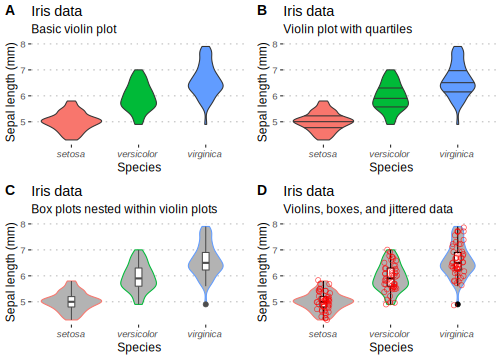
\includegraphics[width=0.7\linewidth]{04-graphics_files/figure-latex/graphics-plot8-1} \caption{Variations of violin plots.}\label{fig:graphics-plot8}
\end{figure}

\hypertarget{exercises-1}{%
\section{Exercises}\label{exercises-1}}

\hypertarget{exercise-1-1}{%
\subsection{Exercise 1}\label{exercise-1-1}}

Choose a dataset, either one of the many built into R or one of your
own, and create four distinctly different figures. Use
\texttt{ggarrange()} to stitch them together in a meaningful way.

\hypertarget{distributions}{%
\chapter{Distributions}\label{distributions}}

Therefore, we must next learn about the different types of data
distributions we are likely to encounter in the wild.

\hypertarget{discrete-distributions}{%
\section{Discrete distributions}\label{discrete-distributions}}

A discrete random variable has a finite or countable number of possible
values. As the name suggests, it models integer data. Below we provide
options to generate and visualise data belonging to several classes of
discrete distributions. Later (Chapter 11) we will learn how to
transform these data prior to performing the appropriate statistical
analysis.

\hypertarget{bernoulli-distribution}{%
\subsection{Bernoulli distribution}\label{bernoulli-distribution}}

A Bernoulli random variable, \(x\), takes the value 1 with probability
\(p\) and the value 0 with probability \(q=1−p\). It is used to
represent data resulting from a \emph{single} experiment with binary
(yes or no; black or white; positive or negative; success or failure;
dead or alive;) outcomes, such as a coin toss---there are only two
options, heads or tails. Nothing else. Here, \(p\) represents the
probability of the one outcome and \(q\) the probability of the other
outcome. The distribution of the possible outcomes, \(x\), is given by:

\[
f(x;p)=
  \begin{cases}
    p, &\text{if}~x=1\\
    1-p, &\text{if}~x=0
  \end{cases}
\]

\hypertarget{binomial-distribution}{%
\subsection{Binomial distribution}\label{binomial-distribution}}

A binomial random variable, \(x\), is the sum of \(n\) independent
Bernoulli random variables with parameter \(p\). This data distribution
results from repeating identical experiments that produce a binary
outcome with probability \(p\) a specified number of times, and choosing
\(n\) samples at random. As such, it represents a collection of
Bernoulli trials.

\[f(x;n,p)= {n\choose x}p^{x}(1-p)^{n-x}\]

\hypertarget{negative-binomial-distribution}{%
\subsection{Negative binomial
distribution}\label{negative-binomial-distribution}}

A negative binomial random variable, \(x\), counts the number of
successes in a sequence of independent Bernoulli trials with probability
\(p\) before \(r\) failures occur. This distribution could for example
be used to predict the number of heads that result from a series of coin
tosses before three tails are observed:

\[f(x;n,r,p)= {x+r-1\choose x}p^{x}(1-p)^{r}\]

where \(x\) is the number of successes, \(r\) is the number of failures,
and \(p\) is the probability of success

\hypertarget{geometric-distribution}{%
\subsection{Geometric distribution}\label{geometric-distribution}}

A geometric random variable, \(x\), represents the number of trials that
are required to observe a single success. Each trial is independent and
has success probability \(p\). As an example, the geometric distribution
is useful to model the number of times a die must be tossed in order for
a six to be observed. It is given by:

\[f(x;p)=(1-p)^{x}p\]

\hypertarget{poisson-distribution}{%
\subsection{Poisson distribution}\label{poisson-distribution}}

A Poisson random variable, \(x\), tallies the number of events occurring
in a fixed interval of time or space, given that these events occur with
an average rate \(\lambda\). Poisson distributions can be used to model
events such as meteor showers and or number of people entering a
shopping mall. This equation describes the Poison distribution:

\[f(x;\lambda)=\frac{\lambda^{x}e^{-\lambda}}{x!}\]

\hypertarget{continuous-distributions}{%
\section{Continuous distributions}\label{continuous-distributions}}

\hypertarget{normal-distribution}{%
\subsection{Normal distribution}\label{normal-distribution}}

Another name for this kind of distribution is a Gaussian distribution. A
random sample with a Gaussian distribution is normally distributed.
These values are identically distributed and independent---we say they
are independent and identically distributed random variables (i.i.d.),
and they have an expected mean given by \(\mu\) (or \(\hat{x}\) in
Chapter 3.2.1) and a finite variance given by \(\sigma^{2}\) (or
\(S^{2}\) in Chapter 3.3.1); if the number of samples drawn from a
population is sufficiently large, the estimated mean and SD will be
indistinguishable from the population (as per the central limit
theorem).

\begin{figure}[h!]
\begin{center}
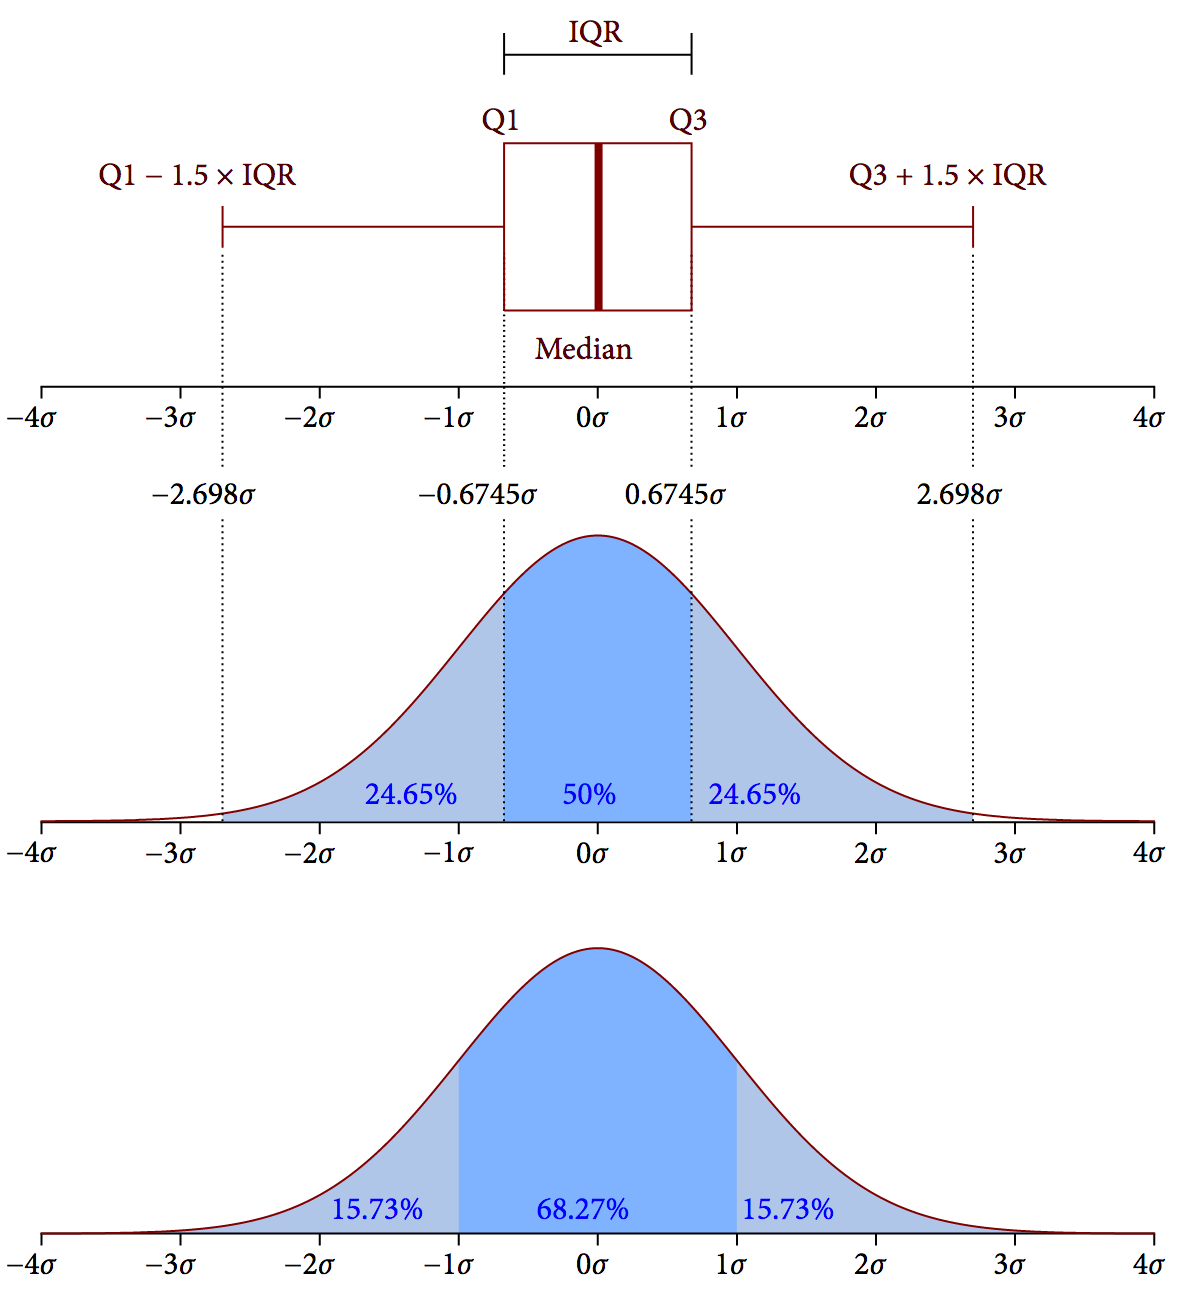
\includegraphics[width=0.7\linewidth]{figures/Boxplot_vs_PDF.png}
\end{center}
\caption{Boxplot and probability density function of a normal distribution. Credit: Wikipedia.}
\end{figure}

\hypertarget{uniform-distribution}{%
\subsection{Uniform distribution}\label{uniform-distribution}}

The continuous uniform distribution is sometime called a rectangular
distribution. Simply, it states that all measurements of the same
magnitude included with this distribution are equally probable. This is
basically random numbers.

\hypertarget{student-t-distribution}{%
\subsection{Student T distribution}\label{student-t-distribution}}

This is a continuous probability distribution that arises when
estimating the mean of a normally distributed population in situations
where the sample size is small and population standard deviation is
unknown. It is used in the statistical significance testing between the
means of different sets of samples, and not much so in the modelling of
natural phenomena.

\hypertarget{chi-squared-distribution}{%
\subsection{Chi-squared distribution}\label{chi-squared-distribution}}

Mostly used in hypothesis testing, but not to encapsulate the
distribution of data drawn to represent natural phenomena.

\hypertarget{exponential-distribution}{%
\subsection{Exponential distribution}\label{exponential-distribution}}

This is a probability distribution that describes the time between
events in a Poisson point process, i.e., a process in which events occur
continuously and independently at a constant average rate.

\hypertarget{f-distribution}{%
\subsection{F distribution}\label{f-distribution}}

\hypertarget{gamma-distribution}{%
\subsection{Gamma distribution}\label{gamma-distribution}}

\hypertarget{beta-distribution}{%
\subsection{Beta distribution}\label{beta-distribution}}

\hypertarget{paranormal-distributions}{%
\subsection{Paranormal distributions}\label{paranormal-distributions}}

\begin{figure}[h!]
\begin{center}
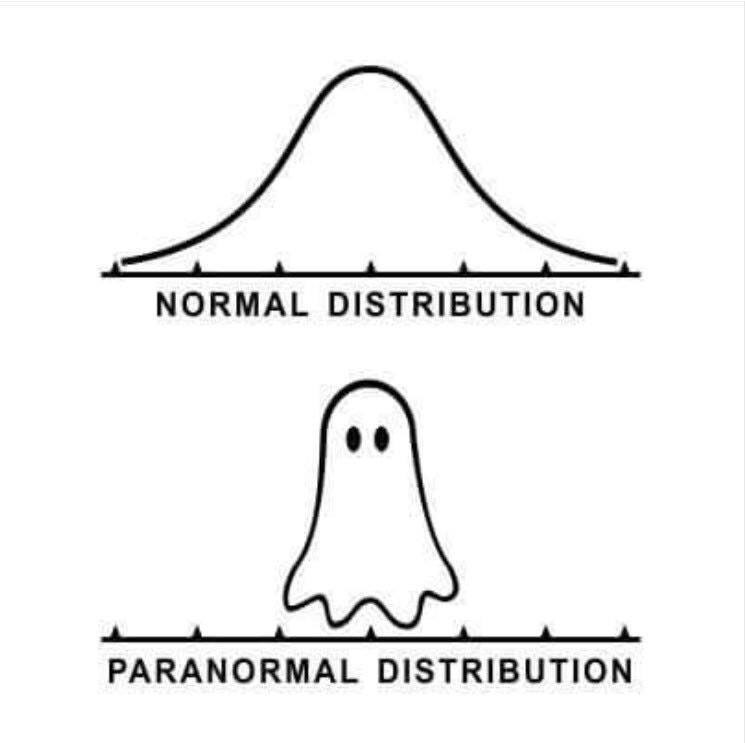
\includegraphics[width=0.7\linewidth]{figures/paranormal_distributions.jpeg}
\end{center}
\end{figure}

\hypertarget{finding-ones-data-distribution}{%
\section{Finding one's data
distribution}\label{finding-ones-data-distribution}}

data belonging to a sample will never exactly follow a specific
distribution, even when the test for normality says it does---there will
always be a small probability that they are non-normal and is in fact
better described by some other distribution. In other words, data are
only \emph{compatible} with a certain distribution, and one can never
answer the question \enquote{Does my data follow the distribution xy
exactly?} as simply as providing a yes/no answer. So what now? How does
one find one's data distribution? We can use the \emph{Cullen and Frey
graph} function that lives in the \textbf{fitdistrplus} package. This
graph tells us whether the skewness and kurtosis of our data are
consistent with that of a particular distribution. We will demonstrate
by generating various data distributions and testing them using the
Cullen and Frey graph.

\begin{Shaded}
\begin{Highlighting}[]
\KeywordTok{library}\NormalTok{(fitdistrplus)}
\end{Highlighting}
\end{Shaded}

\begin{verbatim}
## Loading required package: MASS
\end{verbatim}

\begin{verbatim}
## Loading required package: survival
\end{verbatim}

\begin{verbatim}
## Loading required package: methods
\end{verbatim}

\begin{Shaded}
\begin{Highlighting}[]
\KeywordTok{library}\NormalTok{(logspline)}

\CommentTok{# Generate log-normal data}
\NormalTok{y <-}\StringTok{ }\KeywordTok{c}\NormalTok{(}\FloatTok{37.50}\NormalTok{,}\FloatTok{46.79}\NormalTok{,}\FloatTok{48.30}\NormalTok{,}\FloatTok{46.04}\NormalTok{,}\FloatTok{43.40}\NormalTok{,}\FloatTok{39.25}\NormalTok{,}\FloatTok{38.49}\NormalTok{,}\FloatTok{49.51}\NormalTok{,}\FloatTok{40.38}\NormalTok{,}\FloatTok{36.98}\NormalTok{,}\FloatTok{40.00}\NormalTok{,}
\FloatTok{38.49}\NormalTok{,}\FloatTok{37.74}\NormalTok{,}\FloatTok{47.92}\NormalTok{,}\FloatTok{44.53}\NormalTok{,}\FloatTok{44.91}\NormalTok{,}\FloatTok{44.91}\NormalTok{,}\FloatTok{40.00}\NormalTok{,}\FloatTok{41.51}\NormalTok{,}\FloatTok{47.92}\NormalTok{,}\FloatTok{36.98}\NormalTok{,}\FloatTok{43.40}\NormalTok{,}
\FloatTok{42.26}\NormalTok{,}\FloatTok{41.89}\NormalTok{,}\FloatTok{38.87}\NormalTok{,}\FloatTok{43.02}\NormalTok{,}\FloatTok{39.25}\NormalTok{,}\FloatTok{40.38}\NormalTok{,}\FloatTok{42.64}\NormalTok{,}\FloatTok{36.98}\NormalTok{,}\FloatTok{44.15}\NormalTok{,}\FloatTok{44.91}\NormalTok{,}\FloatTok{43.40}\NormalTok{,}
\FloatTok{49.81}\NormalTok{,}\FloatTok{38.87}\NormalTok{,}\FloatTok{40.00}\NormalTok{,}\FloatTok{52.45}\NormalTok{,}\FloatTok{53.13}\NormalTok{,}\FloatTok{47.92}\NormalTok{,}\FloatTok{52.45}\NormalTok{,}\FloatTok{44.91}\NormalTok{,}\FloatTok{29.54}\NormalTok{,}\FloatTok{27.13}\NormalTok{,}\FloatTok{35.60}\NormalTok{,}
\FloatTok{45.34}\NormalTok{,}\FloatTok{43.37}\NormalTok{,}\FloatTok{54.15}\NormalTok{,}\FloatTok{42.77}\NormalTok{,}\FloatTok{42.88}\NormalTok{,}\FloatTok{44.26}\NormalTok{,}\FloatTok{27.14}\NormalTok{,}\FloatTok{39.31}\NormalTok{,}\FloatTok{24.80}\NormalTok{,}\FloatTok{16.62}\NormalTok{,}\FloatTok{30.30}\NormalTok{,}
\FloatTok{36.39}\NormalTok{,}\FloatTok{28.60}\NormalTok{,}\FloatTok{28.53}\NormalTok{,}\FloatTok{35.84}\NormalTok{,}\FloatTok{31.10}\NormalTok{,}\FloatTok{34.55}\NormalTok{,}\FloatTok{52.65}\NormalTok{,}\FloatTok{48.81}\NormalTok{,}\FloatTok{43.42}\NormalTok{,}\FloatTok{52.49}\NormalTok{,}\FloatTok{38.00}\NormalTok{,}
\FloatTok{38.65}\NormalTok{,}\FloatTok{34.54}\NormalTok{,}\FloatTok{37.70}\NormalTok{,}\FloatTok{38.11}\NormalTok{,}\FloatTok{43.05}\NormalTok{,}\FloatTok{29.95}\NormalTok{,}\FloatTok{32.48}\NormalTok{,}\FloatTok{24.63}\NormalTok{,}\FloatTok{35.33}\NormalTok{,}\FloatTok{41.34}\NormalTok{)}

\KeywordTok{par}\NormalTok{(}\DataTypeTok{mfrow =} \KeywordTok{c}\NormalTok{(}\DecValTok{2}\NormalTok{, }\DecValTok{2}\NormalTok{))}
\KeywordTok{plot}\NormalTok{(}\DataTypeTok{x =} \KeywordTok{c}\NormalTok{(}\DecValTok{1}\OperatorTok{:}\KeywordTok{length}\NormalTok{(y)), }\DataTypeTok{y =}\NormalTok{ y)}
\KeywordTok{hist}\NormalTok{(y)}
\KeywordTok{descdist}\NormalTok{(y, }\DataTypeTok{discrete =} \OtherTok{FALSE}\NormalTok{, }\DataTypeTok{boot =} \DecValTok{100}\NormalTok{)}
\end{Highlighting}
\end{Shaded}

\begin{verbatim}
## summary statistics
## ------
## min:  16.62   max:  54.15 
## median:  40.38 
## mean:  40.28434 
## estimated sd:  7.420034 
## estimated skewness:  -0.551717 
## estimated kurtosis:  3.565162
\end{verbatim}

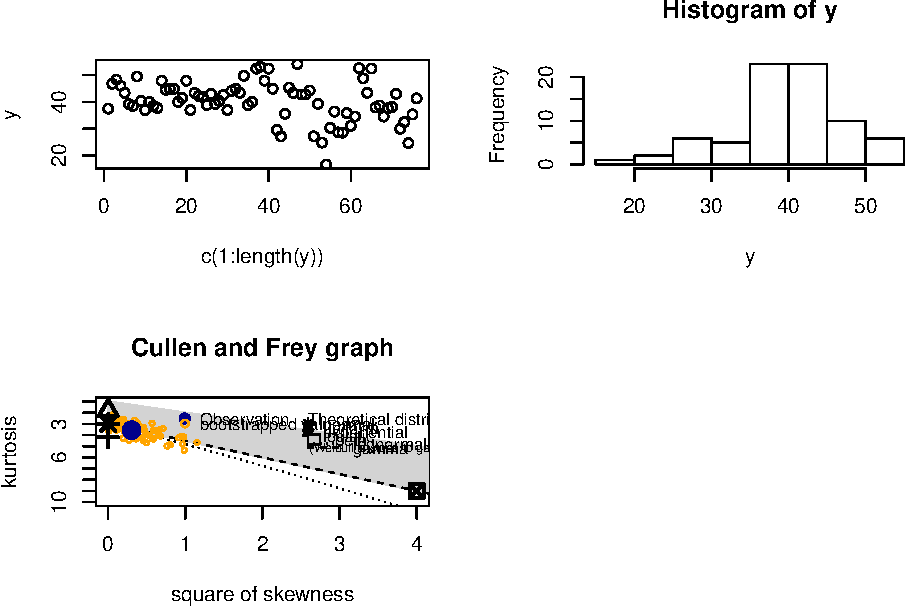
\includegraphics{05-distributions_files/figure-latex/dist-plot1-1.pdf}

\begin{Shaded}
\begin{Highlighting}[]
\CommentTok{# normally distributed data}
\NormalTok{y <-}\StringTok{ }\KeywordTok{rnorm}\NormalTok{(}\DecValTok{100}\NormalTok{, }\DecValTok{13}\NormalTok{, }\DecValTok{2}\NormalTok{)}
\KeywordTok{par}\NormalTok{(}\DataTypeTok{mfrow =} \KeywordTok{c}\NormalTok{(}\DecValTok{2}\NormalTok{, }\DecValTok{2}\NormalTok{))}
\KeywordTok{plot}\NormalTok{(}\DataTypeTok{x =} \KeywordTok{c}\NormalTok{(}\DecValTok{1}\OperatorTok{:}\DecValTok{100}\NormalTok{), }\DataTypeTok{y =}\NormalTok{ y)}
\KeywordTok{hist}\NormalTok{(y)}
\KeywordTok{descdist}\NormalTok{(y, }\DataTypeTok{discrete =} \OtherTok{FALSE}\NormalTok{)}
\end{Highlighting}
\end{Shaded}

\begin{verbatim}
## summary statistics
## ------
## min:  8.503248   max:  18.29135 
## median:  13.35981 
## mean:  13.20023 
## estimated sd:  2.085534 
## estimated skewness:  0.1202547 
## estimated kurtosis:  2.772078
\end{verbatim}

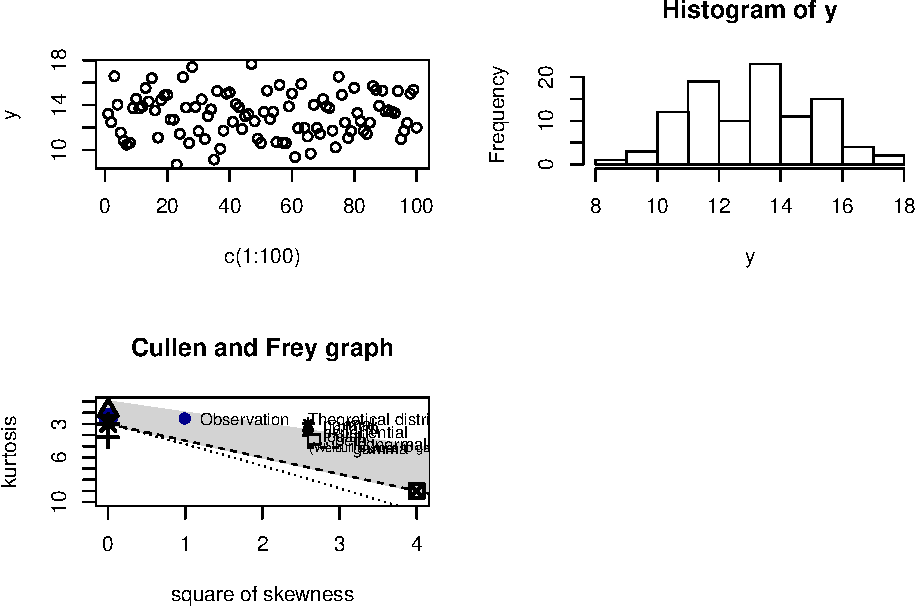
\includegraphics{05-distributions_files/figure-latex/dist-plot2-1.pdf}

\begin{Shaded}
\begin{Highlighting}[]
\CommentTok{# uniformly distributed data}
\NormalTok{y <-}\StringTok{ }\KeywordTok{runif}\NormalTok{(}\DecValTok{100}\NormalTok{)}
\KeywordTok{par}\NormalTok{(}\DataTypeTok{mfrow =} \KeywordTok{c}\NormalTok{(}\DecValTok{2}\NormalTok{, }\DecValTok{2}\NormalTok{))}
\KeywordTok{plot}\NormalTok{(}\DataTypeTok{x =} \KeywordTok{c}\NormalTok{(}\DecValTok{1}\OperatorTok{:}\DecValTok{100}\NormalTok{), }\DataTypeTok{y =}\NormalTok{ y)}
\KeywordTok{hist}\NormalTok{(y)}
\KeywordTok{descdist}\NormalTok{(y, }\DataTypeTok{discrete =} \OtherTok{FALSE}\NormalTok{)}
\end{Highlighting}
\end{Shaded}

\begin{verbatim}
## summary statistics
## ------
## min:  0.005880884   max:  0.993874 
## median:  0.5038945 
## mean:  0.5082694 
## estimated sd:  0.2943109 
## estimated skewness:  -0.01172497 
## estimated kurtosis:  1.898179
\end{verbatim}

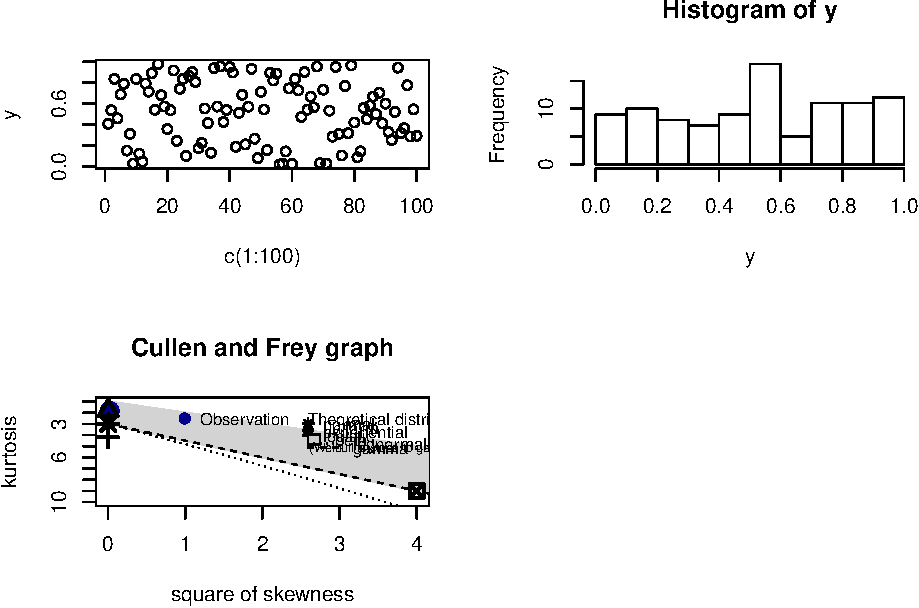
\includegraphics{05-distributions_files/figure-latex/dist-plot3-1.pdf}

\begin{Shaded}
\begin{Highlighting}[]
\CommentTok{# uniformly distributed data}
\NormalTok{y <-}\StringTok{ }\KeywordTok{rexp}\NormalTok{(}\DecValTok{100}\NormalTok{, }\FloatTok{0.7}\NormalTok{)}
\KeywordTok{par}\NormalTok{(}\DataTypeTok{mfrow =} \KeywordTok{c}\NormalTok{(}\DecValTok{2}\NormalTok{, }\DecValTok{2}\NormalTok{))}
\KeywordTok{plot}\NormalTok{(}\DataTypeTok{x =} \KeywordTok{c}\NormalTok{(}\DecValTok{1}\OperatorTok{:}\DecValTok{100}\NormalTok{), }\DataTypeTok{y =}\NormalTok{ y)}
\KeywordTok{hist}\NormalTok{(y)}
\KeywordTok{descdist}\NormalTok{(y, }\DataTypeTok{discrete =} \OtherTok{FALSE}\NormalTok{)}
\end{Highlighting}
\end{Shaded}

\begin{verbatim}
## summary statistics
## ------
## min:  0.03435814   max:  5.51007 
## median:  0.8386743 
## mean:  1.295512 
## estimated sd:  1.210403 
## estimated skewness:  1.434539 
## estimated kurtosis:  4.849173
\end{verbatim}

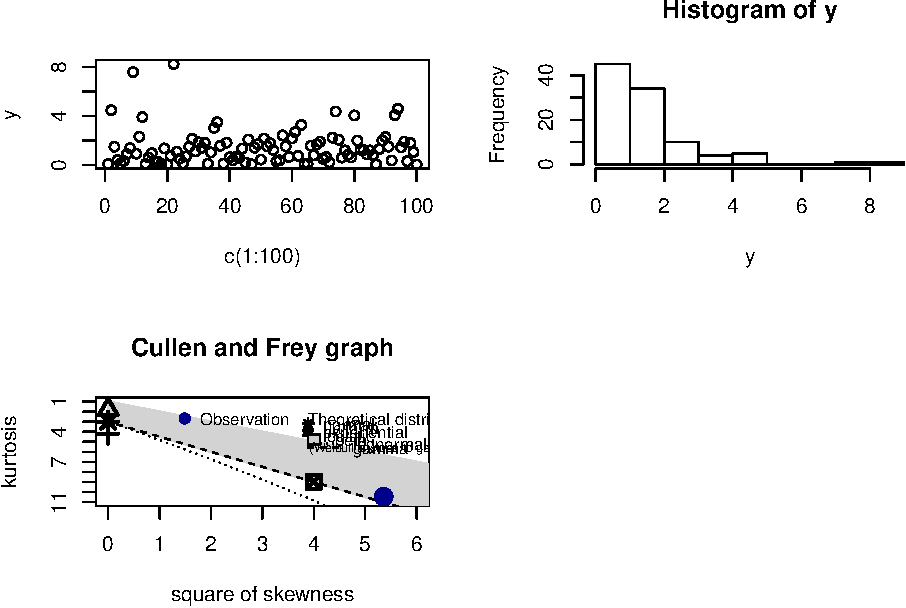
\includegraphics{05-distributions_files/figure-latex/dist-plot4-1.pdf}

There is also a whole bunch of other approaches to use to try and
identify the data distribution. Let us start with the gold standard
first: normal data. We will demonstrate some visualisation approaches.
The one that you already know is a basic histogram; it tells us
something about the distribution's skewness, the tails, the mode(s) of
the data, outliers, etc. Histograms can be compared to shapes associated
with idealistic (simulated) distributions, as we will do here.

\begin{Shaded}
\begin{Highlighting}[]
\NormalTok{y <-}\KeywordTok{rnorm}\NormalTok{(}\DataTypeTok{n =} \DecValTok{200}\NormalTok{, }\DataTypeTok{m =} \DecValTok{13}\NormalTok{, }\DataTypeTok{sd =} \DecValTok{2}\NormalTok{)}
\KeywordTok{par}\NormalTok{(}\DataTypeTok{mfrow =} \KeywordTok{c}\NormalTok{(}\DecValTok{2}\NormalTok{, }\DecValTok{2}\NormalTok{))}
\CommentTok{# using some basic base graphics as ggplot2 is overkill;}
\CommentTok{# we can get a histogram using hist() statement}
\KeywordTok{hist}\NormalTok{(y, }\DataTypeTok{main =} \StringTok{"Histogram of observed data"}\NormalTok{)}
\KeywordTok{plot}\NormalTok{(}\KeywordTok{density}\NormalTok{(y), }\DataTypeTok{main =} \StringTok{"Density estimate of data"}\NormalTok{)}
\KeywordTok{plot}\NormalTok{(}\KeywordTok{ecdf}\NormalTok{(y), }\DataTypeTok{main =} \StringTok{"Empirical cumulative distribution function"}\NormalTok{)}
\CommentTok{# standardise the data}
\NormalTok{z.norm <-}\StringTok{ }\NormalTok{(y }\OperatorTok{-}\StringTok{ }\KeywordTok{mean}\NormalTok{(y)) }\OperatorTok{/}\StringTok{ }\KeywordTok{sd}\NormalTok{(y) }
\CommentTok{# make a qqplot}
\KeywordTok{qqnorm}\NormalTok{(z.norm)}
\CommentTok{# add a 45-degree reference line}
\KeywordTok{abline}\NormalTok{(}\DecValTok{0}\NormalTok{, }\DecValTok{1}\NormalTok{)}
\end{Highlighting}
\end{Shaded}

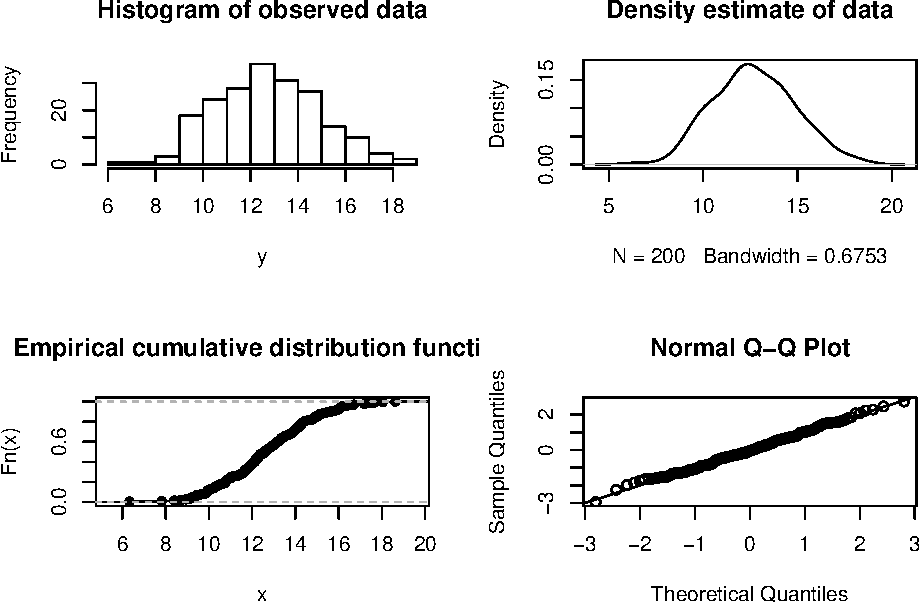
\includegraphics{05-distributions_files/figure-latex/dist-plot5-1.pdf}

Above we have also added a diagonal line to the qqplot. If the sampled
data come from the population with the chosen distribution, the points
should fall approximately along this reference line. The greater the
departure from this reference line, the greater the evidence for the
conclusion that the data set have come from a population with a
different distribution.

\begin{Shaded}
\begin{Highlighting}[]
\CommentTok{# curve(dnorm(100, m = 10, sd = 2), from = 0, to = 20, main = "Normal distribution")}
\CommentTok{# curve(dgamma(100, scale = 1.5, shape = 2), from = 0, to = 15, main = "Gamma distribution")}
\CommentTok{# curve(dweibull(100, scale = 2.5, shape = 1.5), from = 0, to = 15, main = "Weibull distribution")}
\end{Highlighting}
\end{Shaded}

\hypertarget{exercises-2}{%
\section{Exercises}\label{exercises-2}}

\hypertarget{exercise-1-2}{%
\subsection{Exercise 1}\label{exercise-1-2}}

Choose two different datasets and plot them as histograms with density
curves overlayed. Label them with the distribution they appear to be and
stitch them together with \texttt{ggarrange()}.

\hypertarget{inferences-about-one-or-two-populations}{%
\chapter{Inferences about one or two
populations}\label{inferences-about-one-or-two-populations}}

\begin{Shaded}
\begin{Highlighting}[]
\KeywordTok{library}\NormalTok{(tidyverse)}
\KeywordTok{library}\NormalTok{(plotly)}
\end{Highlighting}
\end{Shaded}

At the heart of many basic scientific inquiries is the simple question
\enquote{Is A different from B?} The scientific notation for this
question is:

\begin{itemize}
\tightlist
\item
  H0: Group A is not different from group B.
\item
  H1: Group A is different from group B.
\end{itemize}

More formally, one would say:

\begin{enumerate}
\def\labelenumi{\arabic{enumi}.}
\tightlist
\item
  \(H_{0}: \bar{A} = \bar{B}\) vs.~the alternative hypothesis that
  \(H_{a}: \bar{A} \neq \bar{B}\).
\item
  \(H_{0}: \bar{A} \leq \bar{B}\) vs.~the alternative hypothesis that
  \(H_{a}: \bar{A} > \bar{B}\).
\item
  \(H_{0}: \bar{A} \geq \bar{B}\) vs.~the alternative hypothesis that
  \(H_{a}: \bar{A} < \bar{B}\).
\end{enumerate}

\begin{quote}
\emph{NOTE:} Hypothesis 1 is a two-sided \emph{t}-test and hypotheses 2
and 3 are one-sided tests.
\end{quote}

Biologists typically define the probability of one in twenty (0.05) as
the cutoff level to reject the null hypothesis.

To answer this fundamental question one often uses a \emph{t}-test.
There are several variations of \emph{t}-tests, depending on the nature
of our samples and the type of question being asked:

\begin{itemize}
\tightlist
\item
  \textbf{One-sample \emph{t}-tests:} only one sample set of data that
  we wish to compare against a known population mean:

  \begin{itemize}
  \tightlist
  \item
    one-sided one-sample \emph{t}-tests
  \item
    two-sided one-sample \emph{t}-tests
  \end{itemize}
\item
  \textbf{Two-sample \emph{t}-tests:} the means of two groups are
  compared against each other:

  \begin{itemize}
  \tightlist
  \item
    independent sample \emph{t}-tests

    \begin{itemize}
    \tightlist
    \item
      one-sided two-sample \emph{t}-tests
    \item
      two-sided two-sample \emph{t}-tests
    \end{itemize}
  \item
    paired sample \emph{t}-tests

    \begin{itemize}
    \tightlist
    \item
      one-sided
    \item
      two-sided
    \end{itemize}
  \end{itemize}
\end{itemize}

Before we cover each of these, we need to understand some of the
assumptions behind \emph{t}-tests. We shall cover that next.

\hypertarget{assumptions}{%
\section{Assumptions}\label{assumptions}}

Irrespective of the kind of \emph{t}-test, we have to make a couple of
important assumptions that are \emph{not} guaranteed to be true. In
fact, these assumptions are often violated because real data, especially
biological data, are messy. In order to use a \emph{t}-test to determine
if a significant difference between two sample sets of data exists we
must first establish that:

\begin{itemize}
\tightlist
\item
  the dependent variable must be continuous (i.e.~it is measured at the
  interval or ratio level),
\item
  the observations in the groups being compared are independent of each
  other,
\item
  the data are \textbf{normally distributed}, and
\item
  that the data are \textbf{homoscedastic}, and in particular, that
  there are no outliers.
\end{itemize}

\hypertarget{normality}{%
\subsection{Normality}\label{normality}}

Remember from Chapter 5 what a normal distribution is/looks like? Let's
have a peek below to remind ourselves:

\begin{Shaded}
\begin{Highlighting}[]
\CommentTok{# Random normal data}
\KeywordTok{set.seed}\NormalTok{(}\DecValTok{666}\NormalTok{)}
\NormalTok{r_dat <-}\StringTok{ }\KeywordTok{data.frame}\NormalTok{(}\DataTypeTok{dat =} \KeywordTok{c}\NormalTok{(}\KeywordTok{rnorm}\NormalTok{(}\DataTypeTok{n =} \DecValTok{1000}\NormalTok{, }\DataTypeTok{mean =} \DecValTok{10}\NormalTok{, }\DataTypeTok{sd =} \DecValTok{3}\NormalTok{),}
                            \KeywordTok{rnorm}\NormalTok{(}\DataTypeTok{n =} \DecValTok{1000}\NormalTok{, }\DataTypeTok{mean =} \DecValTok{8}\NormalTok{, }\DataTypeTok{sd =} \DecValTok{2}\NormalTok{)),}
                    \DataTypeTok{sample =} \KeywordTok{c}\NormalTok{(}\KeywordTok{rep}\NormalTok{(}\StringTok{"A"}\NormalTok{, }\DecValTok{1000}\NormalTok{), }\KeywordTok{rep}\NormalTok{(}\StringTok{"B"}\NormalTok{, }\DecValTok{1000}\NormalTok{)))}

\CommentTok{# Create histogram}
\NormalTok{h <-}\StringTok{ }\KeywordTok{ggplot}\NormalTok{(}\DataTypeTok{data =}\NormalTok{ r_dat, }\KeywordTok{aes}\NormalTok{(}\DataTypeTok{x =}\NormalTok{ dat, }\DataTypeTok{fill =}\NormalTok{ sample)) }\OperatorTok{+}
\StringTok{  }\KeywordTok{geom_histogram}\NormalTok{(}\DataTypeTok{position =} \StringTok{"dodge"}\NormalTok{, }\DataTypeTok{binwidth =} \DecValTok{1}\NormalTok{, }\DataTypeTok{alpha =} \FloatTok{0.8}\NormalTok{) }\OperatorTok{+}
\StringTok{  }\KeywordTok{geom_density}\NormalTok{(}\KeywordTok{aes}\NormalTok{(}\DataTypeTok{y =} \DecValTok{1}\OperatorTok{*}\NormalTok{..count.., }\DataTypeTok{fill =}\NormalTok{ sample), }\DataTypeTok{colour =} \OtherTok{NA}\NormalTok{, }\DataTypeTok{alpha =} \FloatTok{0.4}\NormalTok{) }\OperatorTok{+}
\StringTok{  }\KeywordTok{labs}\NormalTok{(}\DataTypeTok{x =} \StringTok{"value"}\NormalTok{)}
\NormalTok{h}
\end{Highlighting}
\end{Shaded}

\begin{figure}
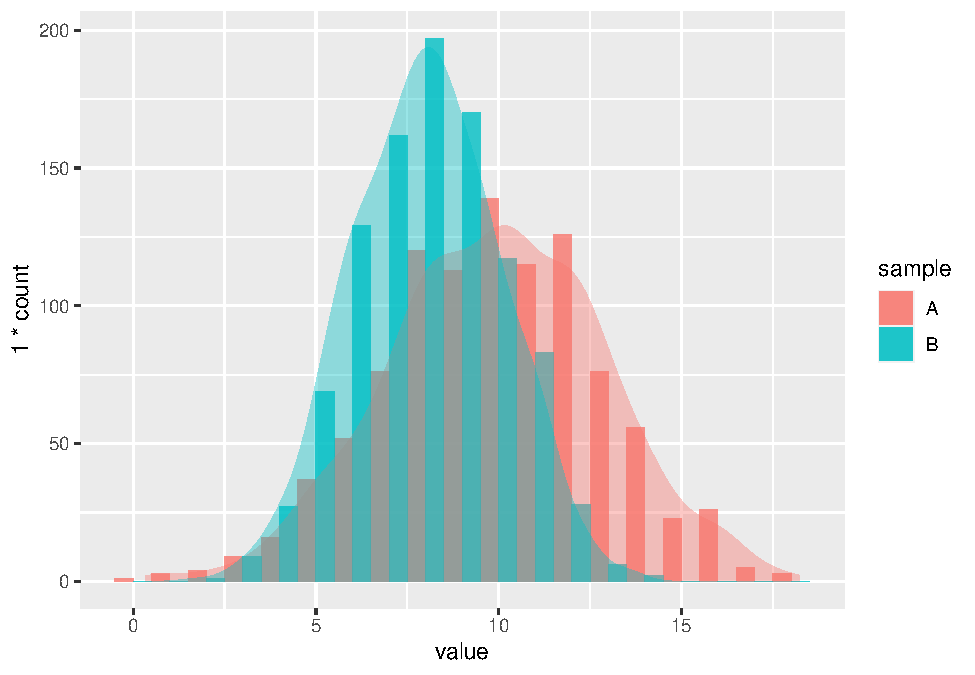
\includegraphics[width=0.7\linewidth]{06-t_tests_files/figure-latex/t-test-plot1-1} \caption{Interactive histogram showing two randomly generated normal distributions.}\label{fig:t-test-plot1}
\end{figure}

Whereas histograms may be a pretty way to check the normality of our
data, there is actually a statistical test for this, which is preferable
to a visual inspection alone. But remember that you should \emph{always}
visualise your data before performing any statistics on them. To check
the normality of the data we use the Shapiro-Wilk test. This test
produces a \(W\) value and a \emph{p}-value. We are only interested in
the \emph{p}-value as this is how we are to determine the normality of
the data. The Shapiro--Wilk test tests the null hypothesis that a sample
\(x_{1},..., x_{n}\) comes from a normally distributed population.
i.e.~that the normality \emph{does not} differ significantly from
normal. If the \emph{p}-value is \textbf{above} 0.05 we may assume the
data to be normally distributed. In order to demonstrate what the output
of \texttt{shapiro.test()} looks like we will run it on all of the
random data we generated.

\begin{Shaded}
\begin{Highlighting}[]
\KeywordTok{shapiro.test}\NormalTok{(r_dat}\OperatorTok{$}\NormalTok{dat)}
\end{Highlighting}
\end{Shaded}

\begin{verbatim}
R> 
R>  Shapiro-Wilk normality test
R> 
R> data:  r_dat$dat
R> W = 0.9942, p-value = 4.649e-07
\end{verbatim}

Note that this shows that the data are \emph{not} normally distributed.
This is because we have incorrectly run this function simultaneously on
two different samples of data. To perform this test correctly, and in
the tidy way, we need to select only the second piece of information
from the \texttt{shapiro.test()} output and ensure that it is presented
as a numeric value:

\begin{Shaded}
\begin{Highlighting}[]
\CommentTok{# we use the square bracket notation to select only the p-value;}
\CommentTok{# had we used `[1]` we'd have gotten W}
\NormalTok{r_dat }\OperatorTok\StringTok{ }
\StringTok{  }\KeywordTok{group_by}\NormalTok{(sample) }\OperatorTok\StringTok{ }
\StringTok{  }\KeywordTok{summarise}\NormalTok{(}\DataTypeTok{norm_dat =} \KeywordTok{as.numeric}\NormalTok{(}\KeywordTok{shapiro.test}\NormalTok{(dat)[}\DecValTok{2}\NormalTok{]))}
\end{Highlighting}
\end{Shaded}

\begin{verbatim}
R> # A tibble: 2 x 2
R>   sample norm_dat
R>   <fct>     <dbl>
R> 1 A         0.375
R> 2 B         0.461
\end{verbatim}

Now we see that our two sample sets are indeed normally distributed.

What if we find that the data are not normally distributed? Although
there are many options, the easiest is to perform a Wilcoxon Rank Sum
test, which is the non-parametric equivalent to a \emph{t}-test (see
Section X). Another option is to transform the data (Chapter 11).

\hypertarget{homoscedasticity}{%
\subsection{Homoscedasticity}\label{homoscedasticity}}

Besides requiring that our data are normally distributed, we must also
ensured that they are homoscedastic. This word means that the
scedasticity (variance) of things are homogeneous (similar). In
practical terms this means that the variance of the samples we are
comparing should not be more than two to four times greater than one
another. In R, we use the function \texttt{var()} to check the variance
in a sample:

\begin{Shaded}
\begin{Highlighting}[]
\NormalTok{r_dat }\OperatorTok\StringTok{ }
\StringTok{  }\KeywordTok{group_by}\NormalTok{(sample) }\OperatorTok\StringTok{ }
\StringTok{  }\KeywordTok{summarise}\NormalTok{(}\DataTypeTok{sample_var =} \KeywordTok{var}\NormalTok{(dat))}
\end{Highlighting}
\end{Shaded}

\begin{verbatim}
R> # A tibble: 2 x 2
R>   sample sample_var
R>   <fct>       <dbl>
R> 1 A            8.72
R> 2 B            3.97
\end{verbatim}

Above we see that the variance of our two samples are homoscedastic
because the variance of one is not more than two to four times greater
than the other.

What if our data are not equal in their variances? This is easier to fix
as the solution is built right into the \emph{t}-test function; all we
need to do is to perform Welch Two Sample \emph{t}-test (the default) in
the \texttt{t.test()} function that we shall use below. If the variances
are equal, we simply perform a normal Student's \emph{t}-test by setting
the argument \texttt{var.equal\ =\ TRUE} in the function call (see
below).

\hypertarget{two-for-one}{%
\subsection{Two for one}\label{two-for-one}}

Because these two assumptions of normality and homoscedasticty are
performed in tandem with one another, it is helpful to have a function
that checks for both simultaneously. Below we see how just such a
function would be written:

\begin{Shaded}
\begin{Highlighting}[]
\NormalTok{two_assum <-}\StringTok{ }\ControlFlowTok{function}\NormalTok{(x) \{}
\NormalTok{  x_var <-}\StringTok{ }\KeywordTok{var}\NormalTok{(x)}
\NormalTok{  x_norm <-}\StringTok{ }\KeywordTok{as.numeric}\NormalTok{(}\KeywordTok{shapiro.test}\NormalTok{(x)[}\DecValTok{2}\NormalTok{])}
\NormalTok{  result <-}\StringTok{ }\KeywordTok{c}\NormalTok{(x_var, x_norm)}
  \KeywordTok{return}\NormalTok{(result)}
\NormalTok{\}}
\end{Highlighting}
\end{Shaded}

To use our new function in a tidy way we use the following code:

\begin{Shaded}
\begin{Highlighting}[]
\NormalTok{r_dat }\OperatorTok\StringTok{ }
\StringTok{  }\KeywordTok{group_by}\NormalTok{(sample) }\OperatorTok\StringTok{ }
\StringTok{  }\KeywordTok{summarise}\NormalTok{(}\DataTypeTok{sample_var =} \KeywordTok{two_assum}\NormalTok{(dat)[}\DecValTok{1}\NormalTok{],}
            \DataTypeTok{sample_norm =} \KeywordTok{two_assum}\NormalTok{(dat)[}\DecValTok{2}\NormalTok{])}
\end{Highlighting}
\end{Shaded}

\begin{verbatim}
R> # A tibble: 2 x 3
R>   sample sample_var sample_norm
R>   <fct>       <dbl>       <dbl>
R> 1 A            8.72       0.375
R> 2 B            3.97       0.461
\end{verbatim}

Do these data meet our assumptions? How do we know this?

Once we have tested our assumptions we may perform a \emph{t}-test to
ascertain whether or not our samples are significantly different from
one another. The base R function for this is \texttt{t.test()}; however,
by utilising the \textbf{\texttt{ggpubr}} package we gain access to
\texttt{compare\_means()}, which allows us to perform any sort of test
that compares sample sets of data and outputs the results as a
dataframe. We will see throughout this and the following chapters why
this is so useful.

\begin{Shaded}
\begin{Highlighting}[]
\KeywordTok{library}\NormalTok{(ggpubr)}
\end{Highlighting}
\end{Shaded}

\hypertarget{one-sample-t-tests}{%
\section{\texorpdfstring{One-sample
\emph{t}-tests}{One-sample t-tests}}\label{one-sample-t-tests}}

Generally when we use a \emph{t}-test it will be a two-sample
\emph{t}-test (see below). Occasionally, however, we may have only one
sample set of data that we wish to compare against a known population
mean, which is generally denoted as \(\mu\), or \texttt{mu} in the
function call to the \emph{t}-test in R:

\begin{Shaded}
\begin{Highlighting}[]
\CommentTok{# create a single sample of random normal data}
\KeywordTok{set.seed}\NormalTok{(}\DecValTok{666}\NormalTok{)}
\NormalTok{r_one <-}\StringTok{ }\KeywordTok{data.frame}\NormalTok{(}\DataTypeTok{dat =} \KeywordTok{rnorm}\NormalTok{(}\DataTypeTok{n =} \DecValTok{20}\NormalTok{, }\DataTypeTok{mean =} \DecValTok{20}\NormalTok{, }\DataTypeTok{sd =} \DecValTok{5}\NormalTok{),}
                    \DataTypeTok{sample =} \StringTok{"A"}\NormalTok{)}

\CommentTok{# check normality}
\KeywordTok{shapiro.test}\NormalTok{(r_one}\OperatorTok{$}\NormalTok{dat)}
\end{Highlighting}
\end{Shaded}

\begin{verbatim}
R> 
R>  Shapiro-Wilk normality test
R> 
R> data:  r_one$dat
R> W = 0.94911, p-value = 0.3538
\end{verbatim}

\begin{Shaded}
\begin{Highlighting}[]
\CommentTok{# No variance to compare}
\CommentTok{# ...}

\CommentTok{# compare random data against a population mean of 20}
\KeywordTok{t.test}\NormalTok{(r_one}\OperatorTok{$}\NormalTok{dat, }\DataTypeTok{mu =} \DecValTok{20}\NormalTok{)}
\end{Highlighting}
\end{Shaded}

\begin{verbatim}
R> 
R>  One Sample t-test
R> 
R> data:  r_one$dat
R> t = 0.0048653, df = 19, p-value = 0.9962
R> alternative hypothesis: true mean is not equal to 20
R> 95 percent confidence interval:
R>  16.91306 23.10133
R> sample estimates:
R> mean of x 
R>  20.00719
\end{verbatim}

\begin{Shaded}
\begin{Highlighting}[]
\CommentTok{# compare random data against a population mean of 30}
\KeywordTok{t.test}\NormalTok{(r_one}\OperatorTok{$}\NormalTok{dat, }\DataTypeTok{mu =} \DecValTok{30}\NormalTok{)}
\end{Highlighting}
\end{Shaded}

\begin{verbatim}
R> 
R>  One Sample t-test
R> 
R> data:  r_one$dat
R> t = -6.7596, df = 19, p-value = 1.858e-06
R> alternative hypothesis: true mean is not equal to 30
R> 95 percent confidence interval:
R>  16.91306 23.10133
R> sample estimates:
R> mean of x 
R>  20.00719
\end{verbatim}

What do the results of these two different tests show? Let's visualise
these data to get a better understanding.

\begin{Shaded}
\begin{Highlighting}[]
\KeywordTok{ggplot}\NormalTok{(}\DataTypeTok{data =}\NormalTok{ r_one, }\KeywordTok{aes}\NormalTok{(}\DataTypeTok{y =}\NormalTok{ dat, }\DataTypeTok{x =}\NormalTok{ sample)) }\OperatorTok{+}
\StringTok{  }\KeywordTok{geom_boxplot}\NormalTok{(}\DataTypeTok{fill =} \StringTok{"lightsalmon"}\NormalTok{) }\OperatorTok{+}
\StringTok{  }\CommentTok{# population  mean (mu) = 20}
\StringTok{  }\KeywordTok{geom_hline}\NormalTok{(}\DataTypeTok{yintercept =} \DecValTok{20}\NormalTok{, }\DataTypeTok{colour =} \StringTok{"blue"}\NormalTok{, }
             \DataTypeTok{size =} \DecValTok{1}\NormalTok{, }\DataTypeTok{linetype =} \StringTok{"dashed"}\NormalTok{) }\OperatorTok{+}
\StringTok{  }\CommentTok{# population  mean (mu) = 30}
\StringTok{  }\KeywordTok{geom_hline}\NormalTok{(}\DataTypeTok{yintercept =} \DecValTok{30}\NormalTok{, }\DataTypeTok{colour =} \StringTok{"red"}\NormalTok{, }
             \DataTypeTok{size =} \DecValTok{1}\NormalTok{, }\DataTypeTok{linetype =} \StringTok{"dashed"}\NormalTok{) }\OperatorTok{+}
\StringTok{  }\KeywordTok{labs}\NormalTok{(}\DataTypeTok{y =} \StringTok{"Value"}\NormalTok{, }\DataTypeTok{x =} \OtherTok{NULL}\NormalTok{) }\OperatorTok{+}
\StringTok{  }\KeywordTok{coord_flip}\NormalTok{()}
\end{Highlighting}
\end{Shaded}

\begin{figure}
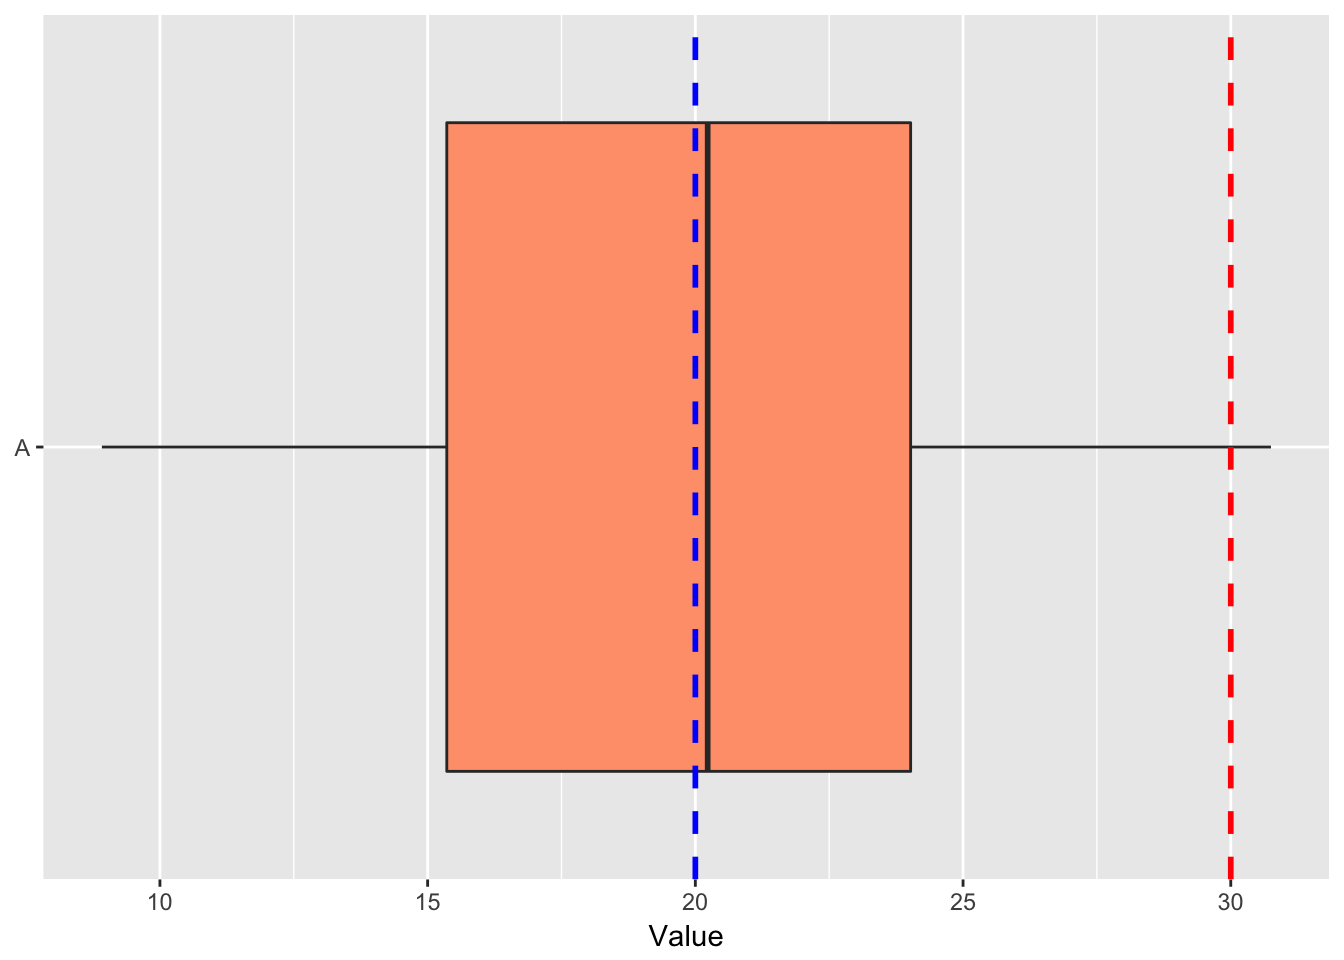
\includegraphics[width=0.7\linewidth]{06-t_tests_files/figure-latex/t-test-plot2-1} \caption{Boxplot of random normal data with. A hypothetical population mean of 20 is shown as a blue line, with the red line showing a mean of 30.}\label{fig:t-test-plot2}
\end{figure}

The boxplot above shows the distribution of our random data against two
potential population means. Does this help now to illustrate the results
of our one-sample \emph{t}-tests?

\hypertarget{one-sided-one-sample-t-tests}{%
\subsection{\texorpdfstring{One-sided one-sample
\emph{t}-tests}{One-sided one-sample t-tests}}\label{one-sided-one-sample-t-tests}}

As we may remember from Chapter 5, a distribution has two tails. When we
are testing for significance we are generally looking for a result that
lays in the far end of either of these tails. Occasionally, however, we
may want to know if the result lays specifically in one of the tails.
Explicitly the leading or trailing tail. For example, is the mean value
of our sample population significantly \emph{greater than} the value
\(\mu\)? Or, is the mean value of our sample population significantly
\emph{less than} the value \(\mu\)? To specify this in R we must add an
argument as seen below:

\begin{Shaded}
\begin{Highlighting}[]
\CommentTok{# check against the trailing tail}
\KeywordTok{t.test}\NormalTok{(r_one}\OperatorTok{$}\NormalTok{dat, }\DataTypeTok{mu =} \DecValTok{30}\NormalTok{, }\DataTypeTok{alternative =} \StringTok{"less"}\NormalTok{)}
\end{Highlighting}
\end{Shaded}

\begin{verbatim}
R> 
R>  One Sample t-test
R> 
R> data:  r_one$dat
R> t = -6.7596, df = 19, p-value = 9.292e-07
R> alternative hypothesis: true mean is less than 30
R> 95 percent confidence interval:
R>      -Inf 22.56339
R> sample estimates:
R> mean of x 
R>  20.00719
\end{verbatim}

\begin{Shaded}
\begin{Highlighting}[]
\CommentTok{# check against the leading tail}
\KeywordTok{t.test}\NormalTok{(r_one}\OperatorTok{$}\NormalTok{dat, }\DataTypeTok{mu =} \DecValTok{30}\NormalTok{, }\DataTypeTok{alternative =} \StringTok{"greater"}\NormalTok{)}
\end{Highlighting}
\end{Shaded}

\begin{verbatim}
R> 
R>  One Sample t-test
R> 
R> data:  r_one$dat
R> t = -6.7596, df = 19, p-value = 1
R> alternative hypothesis: true mean is greater than 30
R> 95 percent confidence interval:
R>  17.451    Inf
R> sample estimates:
R> mean of x 
R>  20.00719
\end{verbatim}

Are these the results we would have expected? Why does the second test
not return a significant result?

\begin{quote}
\textbf{TASK:} Create a visualisation to graphically demonstrate the
outcome of this \emph{t}-test.
\end{quote}

\hypertarget{two-sided-one-sample-t-tests}{%
\subsection{\texorpdfstring{Two-sided one-sample
\emph{t}-tests}{Two-sided one-sample t-tests}}\label{two-sided-one-sample-t-tests}}

In R, the default setting for any comparison of means test is that it is
two-sided so we do not need to state this explicitly. For the sake of
thoroughness let's see how to do this below. Note that the results for
the two following tests are identical:

\begin{Shaded}
\begin{Highlighting}[]
\CommentTok{# R assumes we want a to-sided test}
\KeywordTok{t.test}\NormalTok{(r_one}\OperatorTok{$}\NormalTok{dat, }\DataTypeTok{mu =} \DecValTok{30}\NormalTok{)}
\end{Highlighting}
\end{Shaded}

\begin{verbatim}
R> 
R>  One Sample t-test
R> 
R> data:  r_one$dat
R> t = -6.7596, df = 19, p-value = 1.858e-06
R> alternative hypothesis: true mean is not equal to 30
R> 95 percent confidence interval:
R>  16.91306 23.10133
R> sample estimates:
R> mean of x 
R>  20.00719
\end{verbatim}

\begin{Shaded}
\begin{Highlighting}[]
\CommentTok{# but we can be explicit as we choose}
\KeywordTok{t.test}\NormalTok{(r_one}\OperatorTok{$}\NormalTok{dat, }\DataTypeTok{mu =} \DecValTok{30}\NormalTok{, }\DataTypeTok{alternative =} \StringTok{"two.sided"}\NormalTok{)}
\end{Highlighting}
\end{Shaded}

\begin{verbatim}
R> 
R>  One Sample t-test
R> 
R> data:  r_one$dat
R> t = -6.7596, df = 19, p-value = 1.858e-06
R> alternative hypothesis: true mean is not equal to 30
R> 95 percent confidence interval:
R>  16.91306 23.10133
R> sample estimates:
R> mean of x 
R>  20.00719
\end{verbatim}

\hypertarget{two-sample-t-tests}{%
\section{\texorpdfstring{Two-sample
\emph{t}-tests}{Two-sample t-tests}}\label{two-sample-t-tests}}

A two-sample \emph{t}-test is used when we have samples from two
different populations that we would like to compare against one another.
This is the most common use of a \emph{t}-test. Two sample
\emph{t}-tests can accommodate samples with equal variances or samples
with unequal variances (as determined by the test for heteroscedasticity
that we performed earlier).

In the case of samples that share the same variance we perform a
classical \emph{t}-test (otherwise known as Student's \emph{t}-test);
the equation to calculate the \emph{t}-statistic is this one:

\[t=\frac{\bar{A}-\bar{B}}{\sqrt{\frac{S^{2}}{n}+\frac{S^{2}}{m}}}\]
\(\bar{A}\) and \(\bar{B}\) are the means for groups \(A\) and \(B\),
respectively; \(n\) and \(m\) are the sample sizes of the two sets of
samples, respectively; and \(S^{2}\) is the pooled variance, which is
calculated as:

\[S^{2}=\frac{(n-1)S_{A}^{2}+(m-1)S_{B}^{2} }{n+m-2}\] The degrees of
freedom, \(d.f.\), in the equation for the shared variance is
\(n_{A}+n_{B}-2\).

When variances are unequal we perform the Welch's \emph{t}-test; Welch's
\emph{t}-statistics is calculated as per this equation:

\[t=\frac{\bar{A}-\bar{B}}{\sqrt{\frac{S^{2}_{A}}{n}+\frac{S^{2}_{B}}{m}}}\]

Above, \(S_{A}\) and \(S_{B}\) are the variances of groups \(A\) and
\(B\), respectively (see Section X). The degrees of freedom to use with
Welch's \emph{t}-test is obtained using the Welch--Satterthwaite
equation as:

\[d.f. = \frac{\left( \frac{S^{2}_{A}}{n}+\frac{S^{2}_{B}}{m} \right)^{2}}{\left( \frac{S^{4}_{A}}{n-1} + \frac{S^{4}_{B}}{m-1} \right)}\]

What do we do with this \emph{t}-statistic? In the olden days we had to
calculate the \(t\)-statistics and the \(d.f.\) by hand. These two
values, the \(d.f.\) and \(t\)-value had to be read off a table of
pre-calculated \(t\)-values, probabilities and degrees of freedom
\href{https://home.ubalt.edu/ntsbarsh/Business-stat/StatistialTables.pdf}{as
in here}. Luckily, the \emph{t}-test function nowadays does this all
automagically. But if you are feeling nostalgic over times that you have
sadly never experienced, please calculate the \(t\)-statistic and the
\(d.f.\) yourself and give the table a go.

Back to the present day and the wonders of modern technology. Let's
generate some new random normal data and test to see if the data
belonging to the two groups differ significantly from one-another.
First, we apply the \emph{t}-test function as usual:

\begin{Shaded}
\begin{Highlighting}[]
\CommentTok{# random normal data}
\KeywordTok{set.seed}\NormalTok{(}\DecValTok{666}\NormalTok{)}
\NormalTok{r_two <-}\StringTok{ }\KeywordTok{data.frame}\NormalTok{(}\DataTypeTok{dat =} \KeywordTok{c}\NormalTok{(}\KeywordTok{rnorm}\NormalTok{(}\DataTypeTok{n =} \DecValTok{20}\NormalTok{, }\DataTypeTok{mean =} \DecValTok{4}\NormalTok{, }\DataTypeTok{sd =} \DecValTok{1}\NormalTok{),}
                            \KeywordTok{rnorm}\NormalTok{(}\DataTypeTok{n =} \DecValTok{20}\NormalTok{, }\DataTypeTok{mean =} \DecValTok{5}\NormalTok{, }\DataTypeTok{sd =} \DecValTok{1}\NormalTok{)),}
                    \DataTypeTok{sample =} \KeywordTok{c}\NormalTok{(}\KeywordTok{rep}\NormalTok{(}\StringTok{"A"}\NormalTok{, }\DecValTok{20}\NormalTok{), }\KeywordTok{rep}\NormalTok{(}\StringTok{"B"}\NormalTok{, }\DecValTok{20}\NormalTok{)))}

\CommentTok{# perform t-test}
\CommentTok{# note how we set the `var.equal` argument to TRUE because we know }
\CommentTok{# our data has the same SD (they are simulated as such!)}
\KeywordTok{t.test}\NormalTok{(dat }\OperatorTok{~}\StringTok{ }\NormalTok{sample, }\DataTypeTok{data =}\NormalTok{ r_two, }\DataTypeTok{var.equal =} \OtherTok{TRUE}\NormalTok{)}
\end{Highlighting}
\end{Shaded}

\begin{verbatim}
R> 
R>  Two Sample t-test
R> 
R> data:  dat by sample
R> t = -1.9544, df = 38, p-value = 0.05805
R> alternative hypothesis: true difference in means is not equal to 0
R> 95 percent confidence interval:
R>  -1.51699175  0.02670136
R> sample estimates:
R> mean in group A mean in group B 
R>        4.001438        4.746584
\end{verbatim}

\begin{Shaded}
\begin{Highlighting}[]
\CommentTok{# if the variances are not equal, simply set `var.equal` to false}
\CommentTok{# and a Welch's t-test will be performed}
\end{Highlighting}
\end{Shaded}

The first argument we see in \texttt{t.test()} is
\texttt{dat\ \textasciitilde{}\ sample}. Usually in R when we see a
\texttt{\textasciitilde{}} (tilde) we are creating what is known as a
formula. A formula tells R how it should look for interactions between
data and factors. For example \texttt{Y\ \textasciitilde{}\ X} reads:
\(Y\) as a function of \(X\). In our code above we see
\texttt{dat\ \textasciitilde{}\ sample}. This means we are telling R
that the \emph{t}-test we want it to perform is when the \texttt{dat}
column is a function of the \texttt{sample} column. In plain English we
are dividing up the \texttt{dat} column into the two different samples
we have, and then running a \emph{t}-test on these samples. Another way
of stating this is that the value of \texttt{dat} depends on the
grouping it belong to (\texttt{A} or \texttt{B}). We will see this same
formula notation cropping up later under ANOVAs, linear models, etc.

Now that we have seen the nitty gritty of how a t-test is meant to work,
click \href{}{here} to watch a visualisation that demonstrates how the
relationships between two different sample sets (based on their mean and
variance) influence the results.

\begin{quote}
\textbf{TASK:} Create a visualisation to graphically demonstrate the
outcome of this \emph{t}-test.
\end{quote}

Now we do the same test using a convenient function that comes with the
\textbf{ggpubr} package, called \texttt{compare\_means()}, to perform
the same \emph{t}-test:

\begin{Shaded}
\begin{Highlighting}[]
\CommentTok{# perform t-test using `compare_means()`}
\CommentTok{# note that compare_means() takes the same arguments as t.test()}
\KeywordTok{compare_means}\NormalTok{(dat }\OperatorTok{~}\StringTok{ }\NormalTok{sample, }\DataTypeTok{data =}\NormalTok{ r_two, }\DataTypeTok{method =} \StringTok{"t.test"}\NormalTok{, }\DataTypeTok{var.equal =} \OtherTok{TRUE}\NormalTok{)}
\end{Highlighting}
\end{Shaded}

\begin{verbatim}
R> # A tibble: 1 x 8
R>   .y.   group1 group2      p  p.adj p.format p.signif method
R>   <chr> <chr>  <chr>   <dbl>  <dbl> <chr>    <chr>    <chr> 
R> 1 dat   A      B      0.0580 0.0580 0.058    ns       T-test
\end{verbatim}

Note above that in order to tell \texttt{compare\_means()} to perform a
\emph{t}-test we feed it the argument \texttt{method\ =\ "t.test"}. The
output is similar to that of the familiar \texttt{t.test()} function
that we used earlier, but the output is more abbreviated and less
useful. Typically, the output of the \emph{t}-tests that we need to
report in the results sections of our papers include the
\(t\)-statistic, the \(P\)-value, and the degrees of freedom, \(d.f.\),
and these are absent from the \texttt{compare\_means()} function's
output.

\hypertarget{one-sided-two-sample-t-tests}{%
\subsection{\texorpdfstring{One-sided two-sample
\emph{t}-tests}{One-sided two-sample t-tests}}\label{one-sided-two-sample-t-tests}}

Just as with the one-sample \emph{t}-tests above, we may also specify
which tail of the distribution we are interested in when we compare the
means of our two samples. We do so by providing the same arguments as
previously:

\begin{Shaded}
\begin{Highlighting}[]
\CommentTok{# is the mean of sample B smaller than that of sample A?}
\KeywordTok{compare_means}\NormalTok{(dat }\OperatorTok{~}\StringTok{ }\NormalTok{sample, }\DataTypeTok{data =}\NormalTok{ r_two, }\DataTypeTok{method =} \StringTok{"t.test"}\NormalTok{, }\DataTypeTok{var.equal =} \OtherTok{TRUE}\NormalTok{, }\DataTypeTok{alternative =} \StringTok{"less"}\NormalTok{)}
\end{Highlighting}
\end{Shaded}

\begin{verbatim}
R> # A tibble: 1 x 8
R>   .y.   group1 group2     p p.adj p.format p.signif method
R>   <chr> <chr>  <chr>  <dbl> <dbl> <chr>    <chr>    <chr> 
R> 1 dat   A      B      0.971 0.971 0.97     ns       T-test
\end{verbatim}

\begin{Shaded}
\begin{Highlighting}[]
\CommentTok{# is the mean of sample B greater than that of sample A?}
\KeywordTok{compare_means}\NormalTok{(dat }\OperatorTok{~}\StringTok{ }\NormalTok{sample, }\DataTypeTok{data =}\NormalTok{ r_two, }\DataTypeTok{method =} \StringTok{"t.test"}\NormalTok{, }\DataTypeTok{var.equal =} \OtherTok{TRUE}\NormalTok{, }\DataTypeTok{alternative =} \StringTok{"greater"}\NormalTok{)}
\end{Highlighting}
\end{Shaded}

\begin{verbatim}
R> # A tibble: 1 x 8
R>   .y.   group1 group2      p  p.adj p.format p.signif method
R>   <chr> <chr>  <chr>   <dbl>  <dbl> <chr>    <chr>    <chr> 
R> 1 dat   A      B      0.0290 0.0290 0.029    *        T-test
\end{verbatim}

What do these results show? Is this surprising?

\hypertarget{two-sided-two-sample-t-tests}{%
\subsection{\texorpdfstring{Two-sided two-sample
\emph{t}-tests}{Two-sided two-sample t-tests}}\label{two-sided-two-sample-t-tests}}

Again, as stated above, the default setting in R for comparisons of
means is that the test is two-sided. If one wants to state this
explicitly it may be done as previously. Note that the results are
identical.

\begin{Shaded}
\begin{Highlighting}[]
\CommentTok{# default settings}
\KeywordTok{compare_means}\NormalTok{(dat }\OperatorTok{~}\StringTok{ }\NormalTok{sample, }\DataTypeTok{data =}\NormalTok{ r_two, }\DataTypeTok{method =} \StringTok{"t.test"}\NormalTok{)}
\end{Highlighting}
\end{Shaded}

\begin{verbatim}
R> # A tibble: 1 x 8
R>   .y.   group1 group2      p  p.adj p.format p.signif method
R>   <chr> <chr>  <chr>   <dbl>  <dbl> <chr>    <chr>    <chr> 
R> 1 dat   A      B      0.0584 0.0584 0.058    ns       T-test
\end{verbatim}

\begin{Shaded}
\begin{Highlighting}[]
\CommentTok{# explicitly state a two-sided test}
\KeywordTok{compare_means}\NormalTok{(dat }\OperatorTok{~}\StringTok{ }\NormalTok{sample, }\DataTypeTok{data =}\NormalTok{ r_two, }\DataTypeTok{method =} \StringTok{"t.test"}\NormalTok{, }\DataTypeTok{alternative =} \StringTok{"two.sided"}\NormalTok{)}
\end{Highlighting}
\end{Shaded}

\begin{verbatim}
R> # A tibble: 1 x 8
R>   .y.   group1 group2      p  p.adj p.format p.signif method
R>   <chr> <chr>  <chr>   <dbl>  <dbl> <chr>    <chr>    <chr> 
R> 1 dat   A      B      0.0584 0.0584 0.058    ns       T-test
\end{verbatim}

\hypertarget{paired-t-tests}{%
\section{\texorpdfstring{Paired
\emph{t}-tests}{Paired t-tests}}\label{paired-t-tests}}

Paired \emph{t}-tests are done when comparing matched samples, and in
other words, when our second assumption of \emph{t}-tests is violated:
the observations are independent of one another---in paired samples,
clearly they are not independent. This test is also sometimes called a
dependent sample \emph{t}-test.

For example, we design a survey to determine if, in a group of 20
people, individuals' right arms differ in length from that of their left
arms. For person A, we measure her right arm and her left arm. For
person B we measure his right arm and his left arm. So we go all the way
to person 20. A right arm belonging with one individual is always
matched against a left arm in the same individual. The samples are
paired so we use a paired \emph{t}-test. Another example: we follow the
growth of a sample of 20 piglets over three weeks to see if they weigh
more after three weeks than they did at the start of the assessment
period. We measure the first piglet, named Halal, at the start of the
three week period and again after. We do the same for the second piglet,
Kosher. And so it goes. Each piglet has a paired set of measurements,
one before matched with one after. In both these examples the data in
the two groups (left arm and right arm; or before and after) are not
independent, so we need to account for this in the analysis. In
practice, how do we perform such a \emph{t}-test? Who can think of a
dataset we've used in the past that we would use a paired \emph{t}-test
for?

\begin{Shaded}
\begin{Highlighting}[]
\KeywordTok{compare_means}\NormalTok{(dat }\OperatorTok{~}\StringTok{ }\NormalTok{sample, }\DataTypeTok{data =}\NormalTok{ r_two, }\DataTypeTok{method =} \StringTok{"t.test"}\NormalTok{, }\DataTypeTok{paired =} \OtherTok{TRUE}\NormalTok{)}
\end{Highlighting}
\end{Shaded}

\begin{verbatim}
R> # A tibble: 1 x 8
R>   .y.   group1 group2      p  p.adj p.format p.signif method
R>   <chr> <chr>  <chr>   <dbl>  <dbl> <chr>    <chr>    <chr> 
R> 1 dat   A      B      0.0391 0.0391 0.039    *        T-test
\end{verbatim}

\hypertarget{comparison-of-two-population-proportions}{%
\section{Comparison of two population
proportions}\label{comparison-of-two-population-proportions}}

All of the tests we covered above are designed to deal with continuous
data, such as fish lengths or chlorophyll content. If we want to compare
proportions (probabilities of success) of different samples against each
other, or some known population mean, we need \texttt{prop.test()}.
Let's create a dummy dataset to get a better idea of how this function
works. Below we create some data showing the result of placing two
different subjects, Jack and Jill, in separate sealed rooms for two
hours (120 minutes). Once every minute a mosquito is let into the room
before being extracted again. The columns \texttt{yes} and \texttt{no}
show if the mosquito bit the subject during that one minute. Who says
science can't be fun!

\begin{Shaded}
\begin{Highlighting}[]
\NormalTok{mosquito <-}\StringTok{ }\KeywordTok{matrix}\NormalTok{(}\KeywordTok{c}\NormalTok{(}\DecValTok{70}\NormalTok{, }\DecValTok{85}\NormalTok{, }\DecValTok{50}\NormalTok{, }\DecValTok{35}\NormalTok{), }\DataTypeTok{ncol =} \DecValTok{2}\NormalTok{)}
\KeywordTok{colnames}\NormalTok{(mosquito) <-}\StringTok{ }\KeywordTok{c}\NormalTok{(}\StringTok{"yes"}\NormalTok{, }\StringTok{"no"}\NormalTok{)}
\KeywordTok{rownames}\NormalTok{(mosquito) <-}\StringTok{ }\KeywordTok{c}\NormalTok{(}\StringTok{"Jack"}\NormalTok{, }\StringTok{"Jill"}\NormalTok{)}
\NormalTok{mosquito}
\end{Highlighting}
\end{Shaded}

\begin{verbatim}
R>      yes no
R> Jack  70 50
R> Jill  85 35
\end{verbatim}

\hypertarget{one-sample-and-two-sample-tests}{%
\subsection{One-sample and two-sample
tests}\label{one-sample-and-two-sample-tests}}

As with \emph{t}-tests, proportion tests may also be based on one
sample, or two. If we have only one sample we must specify the total
number of trials as well as what the expected population probability of
success is. Because these are individual values, and not matrices, we
will show what this would look like without using any objects but will
rather give each argument within \texttt{prop.test()} a single exact
value. In the arguments within \texttt{prop.test()}, \texttt{x} denotes
the number of successes recorded, \texttt{n} shows the total number of
individual trials performed, and \texttt{p} is the expected probability.
It is easiest to consider this as though it were a series of 100 coin
tosses.

\begin{Shaded}
\begin{Highlighting}[]
\CommentTok{# When the probability matches the population}
\KeywordTok{prop.test}\NormalTok{(}\DataTypeTok{x =} \DecValTok{45}\NormalTok{, }\DataTypeTok{n =} \DecValTok{100}\NormalTok{, }\DataTypeTok{p =} \FloatTok{0.5}\NormalTok{)}
\end{Highlighting}
\end{Shaded}

\begin{verbatim}
R> 
R>  1-sample proportions test with continuity correction
R> 
R> data:  45 out of 100, null probability 0.5
R> X-squared = 0.81, df = 1, p-value = 0.3681
R> alternative hypothesis: true p is not equal to 0.5
R> 95 percent confidence interval:
R>  0.3514281 0.5524574
R> sample estimates:
R>    p 
R> 0.45
\end{verbatim}

\begin{Shaded}
\begin{Highlighting}[]
\CommentTok{# When it doesn't}
\KeywordTok{prop.test}\NormalTok{(}\DataTypeTok{x =} \DecValTok{33}\NormalTok{, }\DataTypeTok{n =} \DecValTok{100}\NormalTok{, }\DataTypeTok{p =} \FloatTok{0.5}\NormalTok{)}
\end{Highlighting}
\end{Shaded}

\begin{verbatim}
R> 
R>  1-sample proportions test with continuity correction
R> 
R> data:  33 out of 100, null probability 0.5
R> X-squared = 10.89, df = 1, p-value = 0.0009668
R> alternative hypothesis: true p is not equal to 0.5
R> 95 percent confidence interval:
R>  0.2411558 0.4320901
R> sample estimates:
R>    p 
R> 0.33
\end{verbatim}

If we have two samples that we would like to compare against one another
we enter them into the function as follows:

\begin{Shaded}
\begin{Highlighting}[]
\CommentTok{# NB: Note that the `mosquito` data are a matrix, NOT a data.frame}
\KeywordTok{prop.test}\NormalTok{(mosquito)}
\end{Highlighting}
\end{Shaded}

\begin{verbatim}
R> 
R>  2-sample test for equality of proportions with continuity
R>  correction
R> 
R> data:  mosquito
R> X-squared = 3.5704, df = 1, p-value = 0.05882
R> alternative hypothesis: two.sided
R> 95 percent confidence interval:
R>  -0.253309811  0.003309811
R> sample estimates:
R>    prop 1    prop 2 
R> 0.5833333 0.7083333
\end{verbatim}

Do mosquito's bite Jack and Jill at different proportions?

\hypertarget{one-sided-and-two-sided-tests}{%
\subsection{One-sided and two-sided
tests}\label{one-sided-and-two-sided-tests}}

AS with all other tests that compare values, proportion tests may be
specified as either one or two-sided. Just to be clear, the default
setting for \texttt{prop.test()}, like everything else, is a two-sided
test. See code below to confirm that the results are identical with or
without the added argument:

\begin{Shaded}
\begin{Highlighting}[]
\CommentTok{# Default}
\KeywordTok{prop.test}\NormalTok{(mosquito)}
\end{Highlighting}
\end{Shaded}

\begin{verbatim}
R> 
R>  2-sample test for equality of proportions with continuity
R>  correction
R> 
R> data:  mosquito
R> X-squared = 3.5704, df = 1, p-value = 0.05882
R> alternative hypothesis: two.sided
R> 95 percent confidence interval:
R>  -0.253309811  0.003309811
R> sample estimates:
R>    prop 1    prop 2 
R> 0.5833333 0.7083333
\end{verbatim}

\begin{Shaded}
\begin{Highlighting}[]
\CommentTok{# Explicitly state two-sided test}
\KeywordTok{prop.test}\NormalTok{(mosquito, }\DataTypeTok{alternative =} \StringTok{"two.sided"}\NormalTok{)}
\end{Highlighting}
\end{Shaded}

\begin{verbatim}
R> 
R>  2-sample test for equality of proportions with continuity
R>  correction
R> 
R> data:  mosquito
R> X-squared = 3.5704, df = 1, p-value = 0.05882
R> alternative hypothesis: two.sided
R> 95 percent confidence interval:
R>  -0.253309811  0.003309811
R> sample estimates:
R>    prop 1    prop 2 
R> 0.5833333 0.7083333
\end{verbatim}

Should we want to specify only one of the tails to be considered, we do
so precisely the same as with t-tests. Below are examples of what this
code would look like:

\begin{Shaded}
\begin{Highlighting}[]
\CommentTok{# Jack is bit less than Jill}
\KeywordTok{prop.test}\NormalTok{(mosquito, }\DataTypeTok{alternative =} \StringTok{"less"}\NormalTok{)}
\end{Highlighting}
\end{Shaded}

\begin{verbatim}
R> 
R>  2-sample test for equality of proportions with continuity
R>  correction
R> 
R> data:  mosquito
R> X-squared = 3.5704, df = 1, p-value = 0.02941
R> alternative hypothesis: less
R> 95 percent confidence interval:
R>  -1.00000000 -0.01597923
R> sample estimates:
R>    prop 1    prop 2 
R> 0.5833333 0.7083333
\end{verbatim}

\begin{Shaded}
\begin{Highlighting}[]
\CommentTok{# Jack is bit more than Jill}
\KeywordTok{prop.test}\NormalTok{(mosquito, }\DataTypeTok{alternative =} \StringTok{"greater"}\NormalTok{)}
\end{Highlighting}
\end{Shaded}

\begin{verbatim}
R> 
R>  2-sample test for equality of proportions with continuity
R>  correction
R> 
R> data:  mosquito
R> X-squared = 3.5704, df = 1, p-value = 0.9706
R> alternative hypothesis: greater
R> 95 percent confidence interval:
R>  -0.2340208  1.0000000
R> sample estimates:
R>    prop 1    prop 2 
R> 0.5833333 0.7083333
\end{verbatim}

Do these results differ from the two-sided test? What is different?

\hypertarget{a-t-test-workflow}{%
\section{\texorpdfstring{A \emph{t}-test
workflow}{A t-test workflow}}\label{a-t-test-workflow}}

Now that we have seen how to compare the means of two sample sets of
data, let's see what that complete workflow would look like in R. For
this example we will use the \texttt{ecklonia} data from
\href{https://robwschlegel.github.io/Intro_R_Workshop/}{Intro R
Workshop: Data Manipulation, Analysis and Graphing}.

\hypertarget{loading-data}{%
\subsection{Loading data}\label{loading-data}}

Before we can run any analyses we will need to load our data. We are
also going to convert these data from their wide format into a long
format because this is more useful for the rest of our workflow.

\begin{Shaded}
\begin{Highlighting}[]
\NormalTok{ecklonia <-}\StringTok{ }\KeywordTok{read_csv}\NormalTok{(}\StringTok{"data/ecklonia.csv"}\NormalTok{) }\OperatorTok\StringTok{ }
\StringTok{  }\KeywordTok{gather}\NormalTok{(}\DataTypeTok{key =} \StringTok{"variable"}\NormalTok{, }\DataTypeTok{value =} \StringTok{"value"}\NormalTok{, }\OperatorTok{-}\NormalTok{species, }\OperatorTok{-}\NormalTok{site, }\OperatorTok{-}\NormalTok{ID)}
\end{Highlighting}
\end{Shaded}

\hypertarget{visualising-data}{%
\subsection{Visualising data}\label{visualising-data}}

With our data loaded, let's visualise them in order to ensure that these
are indeed the data we are after. Visualising the data will also help us
to formulate a hypothesis.

\begin{Shaded}
\begin{Highlighting}[]
\KeywordTok{ggplot}\NormalTok{(}\DataTypeTok{data =}\NormalTok{ ecklonia, }\KeywordTok{aes}\NormalTok{(}\DataTypeTok{x =}\NormalTok{ variable, }\DataTypeTok{y =}\NormalTok{ value, }\DataTypeTok{fill =}\NormalTok{ site)) }\OperatorTok{+}
\StringTok{  }\KeywordTok{geom_boxplot}\NormalTok{() }\OperatorTok{+}
\StringTok{  }\KeywordTok{coord_flip}\NormalTok{()}
\end{Highlighting}
\end{Shaded}

\textbackslash{}begin\{figure\}
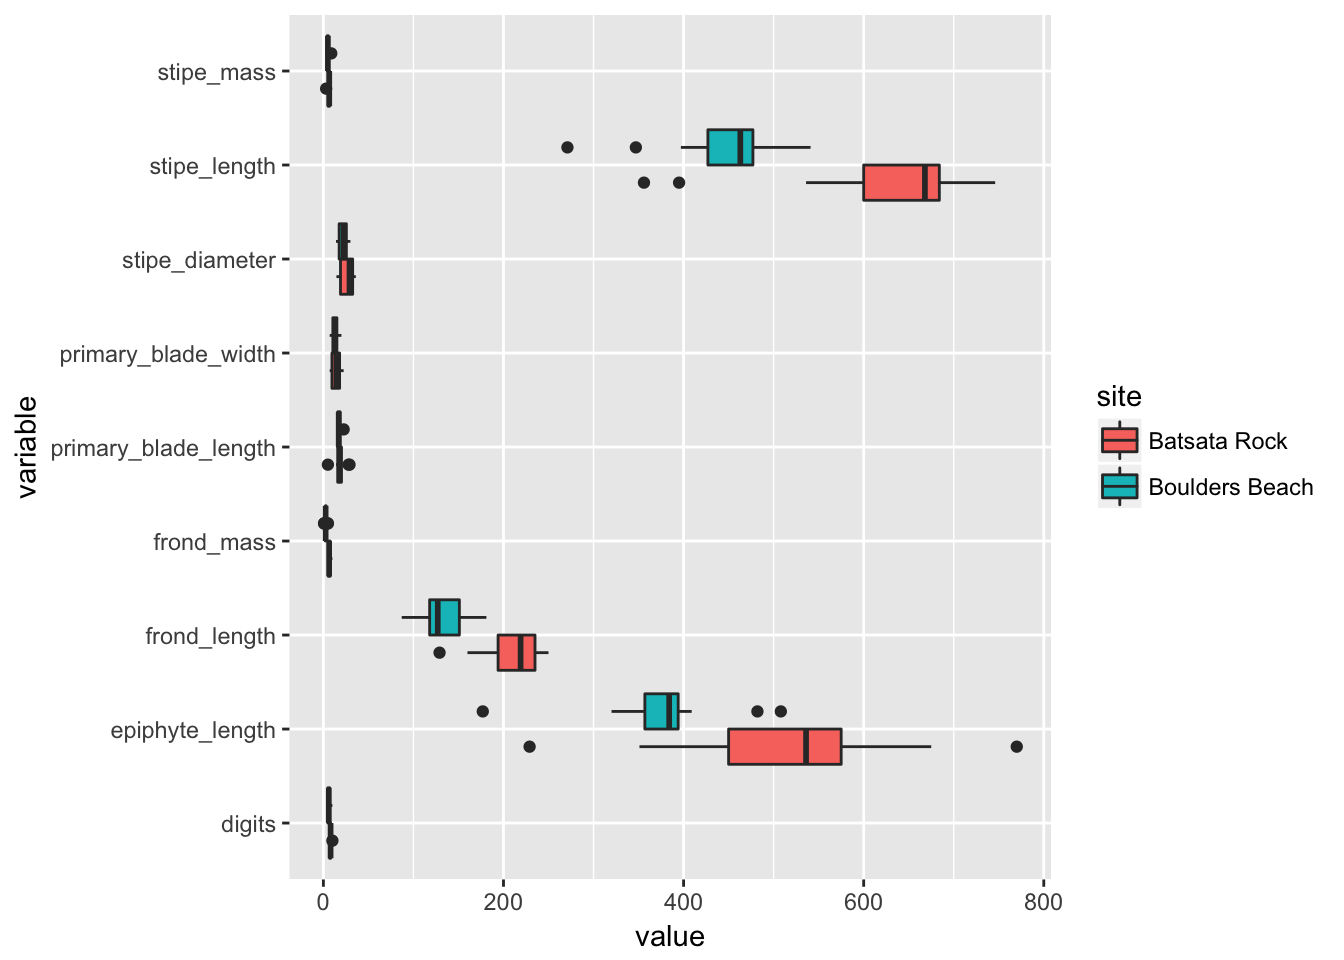
\includegraphics[width=0.7\linewidth]{06-t_tests_files/figure-latex/t-test-plot5-1}
\textbackslash{}caption\{Boxplots showing differences in morphometric
properties of the kelp \emph{Ecklonia maxima} at two sites in False
Bay.\}\label{fig:t-test-plot5} \textbackslash{}end\{figure\}

The first thing we should notice from the figure above is that our
different measurements are on very different scales. This makes
comparing all of our data visually rather challenging. Even given this
complication, one should readily be able to make out that the
measurement values at Batsata Rock appear to be greater than at Boulders
Beach. Within the framework of the scientific process, that is what we
would call an \enquote{observation}, and is the first step towards
formulating a hypothesis. The next step is to refine our observation
into a hypothesis. By what measurement are the kelps greater at one site
than the other?

\hypertarget{formulating-a-hypothesis}{%
\subsection{Formulating a hypothesis}\label{formulating-a-hypothesis}}

Looking at the figure above it appears that for almost all measurements
of length, Batsata Rock far exceeds that of Boulders Beach however, the
stipe masses between the two sites appear to be more similar. Let's pull
out just this variable and create a new boxplot.

\begin{Shaded}
\begin{Highlighting}[]
\CommentTok{# filter the data}
\NormalTok{ecklonia_sub <-}\StringTok{ }\NormalTok{ecklonia }\OperatorTok\StringTok{ }
\StringTok{  }\KeywordTok{filter}\NormalTok{(variable }\OperatorTok{==}\StringTok{ "stipe_mass"}\NormalTok{)}

\CommentTok{# then create a new figure}
\KeywordTok{ggplot}\NormalTok{(}\DataTypeTok{data =}\NormalTok{ ecklonia_sub, }\KeywordTok{aes}\NormalTok{(}\DataTypeTok{x =}\NormalTok{ variable, }\DataTypeTok{y =}\NormalTok{ value, }\DataTypeTok{fill =}\NormalTok{ site)) }\OperatorTok{+}
\StringTok{  }\KeywordTok{geom_boxplot}\NormalTok{() }\OperatorTok{+}
\StringTok{  }\KeywordTok{coord_flip}\NormalTok{() }\OperatorTok{+}
\StringTok{  }\KeywordTok{labs}\NormalTok{(}\DataTypeTok{y =} \StringTok{"stipe mass (kg)"}\NormalTok{, }\DataTypeTok{x =} \StringTok{""}\NormalTok{) }\OperatorTok{+}
\StringTok{  }\KeywordTok{theme}\NormalTok{(}\DataTypeTok{axis.text.y =} \KeywordTok{element_blank}\NormalTok{(),}
        \DataTypeTok{axis.ticks.y =} \KeywordTok{element_blank}\NormalTok{())}
\end{Highlighting}
\end{Shaded}

\textbackslash{}begin\{figure\}
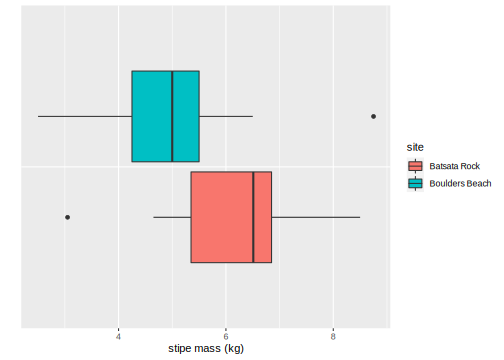
\includegraphics[width=0.7\linewidth]{06-t_tests_files/figure-latex/t-test-plot6-1}
\textbackslash{}caption\{Boxplots showing the difference in stipe mass
(kg) of the kelp \emph{Ecklonia maxima} at two sites in False
Bay.\}\label{fig:t-test-plot6} \textbackslash{}end\{figure\}

Now we have a more interesting comparison at hand. The question I think
of when I look at these data is \enquote{Are the stipe masses at Batsata
Rock greater than at Boulders Beach?}. The hypothesis necessary to
answer this question would look like this:

\begin{itemize}
\tightlist
\item
  H0: Stipe mass at Batsata Rock \textbf{is not} greater than at
  Boulders Beach.
\item
  H1: Stipe mass at Batsata Rock \textbf{is} greater than at Boulders
  Beach.
\end{itemize}

Or more formally:

\begin{itemize}
\tightlist
\item
  \(H_{0}: \bar{A} \leq \bar{B}\)
\item
  \(H_{a}: \bar{A} > \bar{B}\).
\end{itemize}

Which test must we use for this hypothesis?

\hypertarget{choosing-a-test}{%
\subsection{Choosing a test}\label{choosing-a-test}}

Before we can pick the correct statistical test for our hypothesis, we
need to be clear on what it is we are asking. Starting with the data
being used is usually a good first step. As we may see in the above
figure, we have two sample sets that we are comparing. Therefore,
unsurprisingly, we will likely be using a \emph{t}-test. But we're not
done yet. How is it that we are comparing these two sample sets?
Remember from the examples above that there are multiple different ways
to compare two sets of data. For our hypothesis we want to see if the
stipe mass at Batsata Rock is \textbf{greater than} the stipe mass at
Boulders Beach, not just that they are different. Because of this we
will need a one-sided \emph{t}-test. But wait, there's more! We've
zeroed in on which sort of test would be appropriate for our hypothesis,
but before we run it we need to check our assumptions.

\hypertarget{checking-assumptions}{%
\subsection{Checking assumptions}\label{checking-assumptions}}

In case we forgot, here are the assumptions for a \emph{t}-test:

\begin{itemize}
\tightlist
\item
  the dependent variable must be continuous (i.e.~it is measured at the
  interval or ratio level),
\item
  the observations in the groups being compared are independent of each
  other,
\item
  the data are \textbf{normally distributed}, and
\item
  that the data are \textbf{homoscedastic}, and in particular, that
  there are no outliers.
\end{itemize}

We know that the first two assumptions are met because our data are
measurements of mass at two different sites. Before we can run our
one-sided \emph{t}-test we must meet the last two assumptions. Lucky us,
we have a function tat will do that automagically.

\begin{Shaded}
\begin{Highlighting}[]
\NormalTok{ecklonia_sub }\OperatorTok\StringTok{ }
\StringTok{  }\KeywordTok{group_by}\NormalTok{(site) }\OperatorTok\StringTok{ }
\StringTok{  }\KeywordTok{summarise}\NormalTok{(}\DataTypeTok{stipe_mass_var =} \KeywordTok{two_assum}\NormalTok{(value)[}\DecValTok{1}\NormalTok{],}
            \DataTypeTok{stipe_mass_norm =} \KeywordTok{two_assum}\NormalTok{(value)[}\DecValTok{2}\NormalTok{])}
\end{Highlighting}
\end{Shaded}

\begin{verbatim}
R> # A tibble: 2 x 3
R>   site           stipe_mass_var stipe_mass_norm
R>   <chr>                   <dbl>           <dbl>
R> 1 Batsata Rock             2.00           0.813
R> 2 Boulders Beach           2.64           0.527
\end{verbatim}

Lovely. On to the next step.

\hypertarget{running-an-analysis}{%
\subsection{Running an analysis}\label{running-an-analysis}}

With our assumptions checked, we may now analyse our data. We'll see
below how to do this with both of the functions we've learned in this
chapter for comparing means of two sample sets.

\begin{Shaded}
\begin{Highlighting}[]
\CommentTok{# traditional output}
\KeywordTok{t.test}\NormalTok{(value }\OperatorTok{~}\StringTok{ }\NormalTok{site, }\DataTypeTok{data =}\NormalTok{ ecklonia_sub, }\DataTypeTok{var.equal =} \OtherTok{TRUE}\NormalTok{, }\DataTypeTok{alternative =} \StringTok{"greater"}\NormalTok{)}
\end{Highlighting}
\end{Shaded}

\begin{verbatim}
R> 
R>  Two Sample t-test
R> 
R> data:  value by site
R> t = 1.8741, df = 24, p-value = 0.03657
R> alternative hypothesis: true difference in means is greater than 0
R> 95 percent confidence interval:
R>  0.09752735        Inf
R> sample estimates:
R>   mean in group Batsata Rock mean in group Boulders Beach 
R>                     6.116154                     4.996154
\end{verbatim}

\begin{Shaded}
\begin{Highlighting}[]
\CommentTok{# dataframe output}
\KeywordTok{compare_means}\NormalTok{(value }\OperatorTok{~}\StringTok{ }\NormalTok{site, }\DataTypeTok{data =}\NormalTok{ ecklonia_sub, }\DataTypeTok{method =} \StringTok{"t.test"}\NormalTok{, }\DataTypeTok{var.equal =} \OtherTok{TRUE}\NormalTok{, }\DataTypeTok{alternative =} \StringTok{"greater"}\NormalTok{)}
\end{Highlighting}
\end{Shaded}

\begin{verbatim}
R> # A tibble: 1 x 8
R>   .y.   group1         group2            p  p.adj p.format p.signif method
R>   <chr> <chr>          <chr>         <dbl>  <dbl> <chr>    <chr>    <chr> 
R> 1 value Boulders Beach Batsata Rock 0.0366 0.0366 0.037    *        T-test
\end{verbatim}

\hypertarget{interpreting-the-results}{%
\subsection{Interpreting the results}\label{interpreting-the-results}}

We may reject the null hypothesis, that the stipe mass of kelps at
Batsata Rock are not greater than at Boulders Beach, if our
\emph{t}-test returns a \emph{p}-value \(\leq\) 0.05. We must also pay
attention to some of the other results from our \emph{t}-test,
specifically the \emph{t}-value (t) and the degrees of freedom (df) as
these are also needed when we are writing up our results. From all of
the information above, we may accept the alternative hypothesis. But how
do we write that up?

\hypertarget{drawing-conclusions}{%
\subsection{Drawing conclusions}\label{drawing-conclusions}}

There are many ways to present ones findings. Style, without \emph{too
much} flourish, is encouraged as long as certain necessary pieces of
information are provided. The sentence below is a very minimalist
example of how one may conclude this mini research project. A more
thorough explanation would be desirable.

\begin{quote}
The stipe mass (kg) of the kelp \emph{Ecklonia maxima} was found to be
significantly greater at Batsata Rock than at Boulders Beach (\emph{p} =
0.03, \emph{t} = 1.87, df = 24).
\end{quote}

\hypertarget{going-further}{%
\subsection{Going further}\label{going-further}}

But why though? As is often the case in life, and science is no
exception, answers to our questions just create even more questions! Why
would the mass of kelp stipes at one locations in the same body of water
and only a kilometre or so apart be significantly different? It looks
like we are going to need to design a new experiment\ldots{} Masters
thesis anyone?

\hypertarget{exercises-3}{%
\section{Exercises}\label{exercises-3}}

\hypertarget{exercise-1-3}{%
\subsection{Exercise 1}\label{exercise-1-3}}

Find or create your own normally distributed data and think of a
hypothesis you could use a t-test for. Write out the hypothesis, test
it, and write a one sentence conclusion for it. Provide all of the code
used to accomplish this.

\hypertarget{exercise-2}{%
\subsection{Exercise 2}\label{exercise-2}}

Do the same as Exercise 1, but for probability data.

\hypertarget{anova}{%
\chapter{ANOVA}\label{anova}}

Whole big books have been written about Analysis of Variance (ANOVA).
Although there are many ANOVA experimental designs available, biologists
are taught to pay special attention to the design of experiments, and
generally make sure that the experiments are fully factorial (in the
case of two-way or higher ANOVAs) and balanced. For this reason we will
focus in this Introductory Statistics course on one-way and factorial
ANOVAs only.

As \emph{t}-tests, ANOVAs require that some assumptions are met:

\begin{itemize}
\tightlist
\item
  Normally distributed data
\item
  Homogeneity of variances
\item
  Independence of data
\item
  In our case, we will encourage also that the data are balanced
\end{itemize}

If some of the above assumptions are violated, then your course of
action is either to transform the data (if non-normal) or to use a
generalised linear model (also when non-normal), or to use a linear
mixed model (when the assumption on non-independence cannot be
guaranteed). We will get to some of these methods in later chapters.
Linked to the above, ANOVAs are also sensitive to the presence of
outliers (see our earlier discussion about the mean and how it differs
from the median), so we need to ensure that outliers are not present
(they can be removed, and there are many ways of finding them and
eliminating them). If outliers are an important feature of the data,
then a non-parametric test can be used, or some other test that works
well with extreme values can be applied.

Rather than talking about \emph{t}-tests and ANOVAs as separate things,
let us acknowledge that they are similar ways of asking the same
question. That question being, are the means of these two or more things
we want to compare different, or the same? At this stage it is important
to note that the independent variable is categorical (i.e.~a factor
denoting two or more different treatments or sampling conditions) and
that the dependent variable is continuous. You may perhaps be more
familiar with this question when it is presented as a set of hypotheses.

\begin{quote}
H0: Group A is not different from group B.

H1: Group A is different from group B.
\end{quote}

This is a scientific question in the simplest sense. Often, for basic
inquiries such as that posed above, we need to see if one group differs
significantly from another. The way in which we accomplish this is by
looking at the mean and variance within a set of data compared against
another similar set. In order to do so appropriately however we need to
first assume that both sets of data are normally distributed, and that
the variance found within each set of data is similar. These are the two
primary assumptions we learned about in Chapter 6, and if they are met
then we may use parametric tests. We will learn in Chapter 9 what we can
do if these assumptions are not meant and we cannot adequately transform
our data, meaning we will need to use non-parametric tests.

\hypertarget{remember-the-t-test}{%
\section{\texorpdfstring{Remember the
\emph{t}-test}{Remember the t-test}}\label{remember-the-t-test}}

As you know, a \emph{t}-test is used when we want to compare two
different sample sets against one another. This is also known as a
two-factor or two level test. When one wants to compare multiple (more
than two) sample sets against one another an ANOVA is required (see
below). Remember how to perform a \emph{t}-test in R: we will revisit
this test using the \texttt{chicks} data, but only for Diets 1 and 2
from day 21.

\begin{Shaded}
\begin{Highlighting}[]
\CommentTok{# First grab the data}
\NormalTok{chicks <-}\StringTok{ }\KeywordTok{as_tibble}\NormalTok{(ChickWeight)}

\CommentTok{# Then subset out only the sample sets to be compared}
\NormalTok{chicks_sub <-}\StringTok{ }\NormalTok{chicks }\OperatorTok\StringTok{ }
\StringTok{  }\KeywordTok{filter}\NormalTok{(Diet }\OperatorTok\StringTok{ }\KeywordTok{c}\NormalTok{(}\DecValTok{1}\NormalTok{, }\DecValTok{2}\NormalTok{), Time }\OperatorTok{==}\StringTok{ }\DecValTok{21}\NormalTok{)}
\end{Highlighting}
\end{Shaded}

Once we have filtered our data we may now perform the \emph{t}-test.
Traditionally this would be performed with \texttt{t.test()}, but recent
developments in R have made any testing for the comparison of means more
convenient by wrapping everything up into the one single function
\texttt{compare\_means()}. We may use only this one single function for
many of the tests we will perform in this chapter as well as Chapter 9.
To use \texttt{compare\_means()} for a \emph{t}-test we must simply
specify this in the \texttt{method} argument, as seen below:

\begin{Shaded}
\begin{Highlighting}[]
\KeywordTok{compare_means}\NormalTok{(weight }\OperatorTok{~}\StringTok{ }\NormalTok{Diet, }\DataTypeTok{data =}\NormalTok{ chicks_sub, }\DataTypeTok{method =} \StringTok{"t.test"}\NormalTok{)}
\end{Highlighting}
\end{Shaded}

\begin{verbatim}
R> # A tibble: 1 x 8
R>   .y.    group1 group2     p p.adj p.format p.signif method
R>   <chr>  <chr>  <chr>  <dbl> <dbl> <chr>    <chr>    <chr> 
R> 1 weight 1      2      0.218 0.218 0.22     ns       T-test
\end{verbatim}

As one may recall from the previous chapter, whenever we want to give a
formula to a function in R, we use the \texttt{\textasciitilde{}}. The
formula used above, \texttt{weight\ \textasciitilde{}\ Diet}, reads in
plain English as \enquote{weight as a function of diet}. This is perhaps
easier to understand as \enquote{Y as a function of X}. This means that
we are assuming whatever is to the left of the
\texttt{\textasciitilde{}} is the dependant variable, and whatever is to
the right is the independent variable. We then tell
\texttt{compare\_means()} to run a \emph{t}-test on our
\texttt{chicks\_sub} dataframe and it does the rest. We see in the
output above that this function gives us a rather tidy read-out of the
information we require to test a potential hypothesis. Let's take a
moment to look through the help file for this function and see what all
of this means. Did the Diet 1 and 2 produce significantly fatter birds?

\hypertarget{anova-1}{%
\section{ANOVA}\label{anova-1}}

In the \texttt{chicks} data we have four diets, not only two as in the
\emph{t}-test example just performed. Why not then simply do a
\emph{t}-test multiple times, once for each pair of diets given to the
chickens? The problem is that the chances of committing a Type I error
increases as more multiple comparisons are done. So, the overall chance
of rejecting the null hypothesis increases. Why? If one sets
\(\alpha=0.05\) (the significance level below which the null hypothesis
is no longer accepted), one will still reject the null hypothesis 5\% of
the time when it is in fact true (i.e.~when there is no difference
between the groups). When many pairwise comparisons are made, the
probability of rejecting the null hypothesis at least once is higher
because we take this 5\% risk each time we repeat a \emph{t}-test. In
the case of the chicken diets, we would have to perform six
\emph{t}-tests, and the error rate would increase to slightly less than
\(6\times5\%\). If you insist in creating more work for yourself and do
\emph{t}-tests many times, one way to overcome the problem of committing
Type I errors that stems from multiple comparisons is to apply a
Bonferroni correction.

Or better still, we do an ANOVA that controls for these Type I errors so
that it remains at 5\%.

A suitable null hypothesis for our chicken weight data is:

\[H_{0}:\mu_{1}=\mu_{2}=\mu_{3}=\mu_{4}\] where \(\mu_{1...4}\) are the
means of the four diets.

At this point I was very tempted to put many equations here, but I
ommitted them for your sake. Let us turn to some examples.

\hypertarget{single-factor}{%
\subsection{Single factor}\label{single-factor}}

We continue with the chicken data. The \emph{t}-test showed that Diets 1
and 2 resulted in the same chicken masses at the end of the experiment
at Day 21. What about the other two diets? Our null hypothesis is that,
at Day 21, \(\mu_{1}=\mu_{2}=\mu_{3}=\mu_{4}\). Is there a statistical
difference between chickens fed these four diets, or do we retain the
null hypothesis? The R function for an ANOVA is \texttt{aov()}. To look
for significant differences between all four diets on the last day of
sampling we use this one line of code:

\begin{Shaded}
\begin{Highlighting}[]
\NormalTok{chicks.aov1 <-}\StringTok{ }\KeywordTok{aov}\NormalTok{(weight }\OperatorTok{~}\StringTok{ }\NormalTok{Diet, }\DataTypeTok{data =} \KeywordTok{filter}\NormalTok{(chicks, Time }\OperatorTok{==}\StringTok{ }\DecValTok{21}\NormalTok{))}
\KeywordTok{summary}\NormalTok{(chicks.aov1)}
\end{Highlighting}
\end{Shaded}

\begin{verbatim}
R>             Df Sum Sq Mean Sq F value  Pr(>F)   
R> Diet         3  57164   19055   4.655 0.00686 **
R> Residuals   41 167839    4094                   
R> ---
R> Signif. codes:  0 '***' 0.001 '**' 0.01 '*' 0.05 '.' 0.1 ' ' 1
\end{verbatim}

\begin{quote}
\textbf{Task:} What does the outcome say about the chicken masses? Which
ones are different from each other?

\textbf{Task:} Devise a graphical display of this outcome.
\end{quote}

If this seems too easy to be true, it's because we aren't quite done
yet. You could use your graphical display to eyeball where the
significant differences are, or we can turn to a more \enquote{precise}
approach. The next step one could take is to run a Tukey HSD test on the
results of the ANOVA by wrapping \texttt{tukeyHSD()} around
\texttt{aov()}:

\begin{Shaded}
\begin{Highlighting}[]
\KeywordTok{TukeyHSD}\NormalTok{(chicks.aov1)}
\end{Highlighting}
\end{Shaded}

\begin{verbatim}
R>   Tukey multiple comparisons of means
R>     95% family-wise confidence level
R> 
R> Fit: aov(formula = weight ~ Diet, data = filter(chicks, Time == 21))
R> 
R> $Diet
R>          diff        lwr       upr     p adj
R> 2-1  36.95000  -32.11064 106.01064 0.4868095
R> 3-1  92.55000   23.48936 161.61064 0.0046959
R> 4-1  60.80556  -10.57710 132.18821 0.1192661
R> 3-2  55.60000  -21.01591 132.21591 0.2263918
R> 4-2  23.85556  -54.85981 102.57092 0.8486781
R> 4-3 -31.74444 -110.45981  46.97092 0.7036249
\end{verbatim}

The output of \texttt{tukeyHSD()} shows us that pairwise comparisons of
all of the groups we are comparing.

\begin{quote}
\textbf{Task:} Look at the help file for this function to better
understand what the output means.

\textbf{Task:} How does one interpret the results? What does this tell
us about the effect that that different diets has on the chicken weights
at Day 21?

\textbf{Task:} Figure out a way to plot the Tukey HSD outcomes.

\textbf{Task:} Why does the ANOVA return a significant result, but the
Tukey test shows that not all of the groups are significantly different
from one another?

\textbf{Task:} Produce a graphical display of the Tukey HSD result.
\end{quote}

Now that we've seen how to perform a single factor ANOVA, let's watch
some animations that highlight how certain aspects of our data may
affect our results.

\begin{itemize}
\tightlist
\item
  When the
  \href{https://raw.githubusercontent.com/ajsmit/Basic_stats/master/figures/aov_n_slide.avi}{sample
  size} changes
\item
  When the
  \href{https://raw.githubusercontent.com/ajsmit/Basic_stats/master/figures/aov_mean_slide.avi}{mean}
  of one sample changes
\item
  When the
  \href{https://raw.githubusercontent.com/ajsmit/Basic_stats/master/figures/aov_sd_slide.avi}{variance}
  of one sample increases
\end{itemize}

\hypertarget{multiple-factors}{%
\subsection{Multiple factors}\label{multiple-factors}}

What if we have multiple grouping variables, and not just one? In the
case of the chicken data, there is also time that seems to be having an
effect.

\begin{quote}
\textbf{Task:} How is time having an effect?

\textbf{Task:} What hypotheses can we construct around time?
\end{quote}

Let us look at some variations around questions concerning time. We
might ask, at a particular time step, are there differences amongst the
effect due to diet on chicken mass? Let's see when diets are starting
the have an effect by examining the outcomes at times 0, 2, 10, and 21:

\begin{Shaded}
\begin{Highlighting}[]
\KeywordTok{summary}\NormalTok{(}\KeywordTok{aov}\NormalTok{(weight }\OperatorTok{~}\StringTok{ }\NormalTok{Diet, }\DataTypeTok{data =} \KeywordTok{filter}\NormalTok{(chicks, Time }\OperatorTok\StringTok{ }\KeywordTok{c}\NormalTok{(}\DecValTok{0}\NormalTok{))))}
\end{Highlighting}
\end{Shaded}

\begin{verbatim}
R>             Df Sum Sq Mean Sq F value Pr(>F)
R> Diet         3   4.32   1.440   1.132  0.346
R> Residuals   46  58.50   1.272
\end{verbatim}

\begin{Shaded}
\begin{Highlighting}[]
\KeywordTok{summary}\NormalTok{(}\KeywordTok{aov}\NormalTok{(weight }\OperatorTok{~}\StringTok{ }\NormalTok{Diet, }\DataTypeTok{data =} \KeywordTok{filter}\NormalTok{(chicks, Time }\OperatorTok\StringTok{ }\KeywordTok{c}\NormalTok{(}\DecValTok{2}\NormalTok{))))}
\end{Highlighting}
\end{Shaded}

\begin{verbatim}
R>             Df Sum Sq Mean Sq F value  Pr(>F)   
R> Diet         3  158.4   52.81   4.781 0.00555 **
R> Residuals   46  508.1   11.05                   
R> ---
R> Signif. codes:  0 '***' 0.001 '**' 0.01 '*' 0.05 '.' 0.1 ' ' 1
\end{verbatim}

\begin{Shaded}
\begin{Highlighting}[]
\KeywordTok{summary}\NormalTok{(}\KeywordTok{aov}\NormalTok{(weight }\OperatorTok{~}\StringTok{ }\NormalTok{Diet, }\DataTypeTok{data =} \KeywordTok{filter}\NormalTok{(chicks, Time }\OperatorTok\StringTok{ }\KeywordTok{c}\NormalTok{(}\DecValTok{10}\NormalTok{))))}
\end{Highlighting}
\end{Shaded}

\begin{verbatim}
R>             Df Sum Sq Mean Sq F value   Pr(>F)    
R> Diet         3   8314    2771    6.46 0.000989 ***
R> Residuals   45  19304     429                     
R> ---
R> Signif. codes:  0 '***' 0.001 '**' 0.01 '*' 0.05 '.' 0.1 ' ' 1
\end{verbatim}

\begin{Shaded}
\begin{Highlighting}[]
\KeywordTok{summary}\NormalTok{(}\KeywordTok{aov}\NormalTok{(weight }\OperatorTok{~}\StringTok{ }\NormalTok{Diet, }\DataTypeTok{data =} \KeywordTok{filter}\NormalTok{(chicks, Time }\OperatorTok\StringTok{ }\KeywordTok{c}\NormalTok{(}\DecValTok{21}\NormalTok{))))}
\end{Highlighting}
\end{Shaded}

\begin{verbatim}
R>             Df Sum Sq Mean Sq F value  Pr(>F)   
R> Diet         3  57164   19055   4.655 0.00686 **
R> Residuals   41 167839    4094                   
R> ---
R> Signif. codes:  0 '***' 0.001 '**' 0.01 '*' 0.05 '.' 0.1 ' ' 1
\end{verbatim}

\begin{quote}
\textbf{Task:} What do you conclude from the above series of ANOVAs?

\textbf{Task:} What problem is associated with running multiple tests in
the way that we have done here?
\end{quote}

Or we may ask, regardless of diet (i.e.~disregarding the effect of diet
by clumping all chickens together), is time having an effect?

\begin{Shaded}
\begin{Highlighting}[]
\NormalTok{chicks.aov2 <-}\StringTok{ }\KeywordTok{aov}\NormalTok{(weight }\OperatorTok{~}\StringTok{ }\KeywordTok{as.factor}\NormalTok{(Time), }\DataTypeTok{data =} \KeywordTok{filter}\NormalTok{(chicks, Time }\OperatorTok\StringTok{ }\KeywordTok{c}\NormalTok{(}\DecValTok{0}\NormalTok{, }\DecValTok{2}\NormalTok{, }\DecValTok{10}\NormalTok{, }\DecValTok{21}\NormalTok{)))}
\KeywordTok{summary}\NormalTok{(chicks.aov2)}
\end{Highlighting}
\end{Shaded}

\begin{verbatim}
R>                  Df Sum Sq Mean Sq F value Pr(>F)    
R> as.factor(Time)   3 939259  313086   234.8 <2e-16 ***
R> Residuals       190 253352    1333                   
R> ---
R> Signif. codes:  0 '***' 0.001 '**' 0.01 '*' 0.05 '.' 0.1 ' ' 1
\end{verbatim}

\begin{quote}
\textbf{Task:} What do you conclude from the above ANOVA?
\end{quote}

Or, to save ourselves a lot of time and reduce the coding effort, we may
simply run a two-way ANOVA and look at the effects of \texttt{Diet} and
\texttt{Time} simultaneously. To specify the different factors we put
them in our formula and separate them with a \texttt{+}:

\begin{Shaded}
\begin{Highlighting}[]
\KeywordTok{summary}\NormalTok{(}\KeywordTok{aov}\NormalTok{(weight }\OperatorTok{~}\StringTok{ }\NormalTok{Diet }\OperatorTok{+}\StringTok{ }\KeywordTok{as.factor}\NormalTok{(Time), }\DataTypeTok{data =} \KeywordTok{filter}\NormalTok{(chicks, Time }\OperatorTok\StringTok{ }\KeywordTok{c}\NormalTok{(}\DecValTok{0}\NormalTok{, }\DecValTok{21}\NormalTok{))))}
\end{Highlighting}
\end{Shaded}

\begin{verbatim}
R>                 Df Sum Sq Mean Sq F value  Pr(>F)    
R> Diet             3  39595   13198   5.987 0.00091 ***
R> as.factor(Time)  1 734353  734353 333.120 < 2e-16 ***
R> Residuals       90 198402    2204                    
R> ---
R> Signif. codes:  0 '***' 0.001 '**' 0.01 '*' 0.05 '.' 0.1 ' ' 1
\end{verbatim}

\begin{quote}
\textbf{Task:} What question are we asking with the above line of code?
What is the answer? Also, why did we wrap \texttt{Time} in
\texttt{as.factor()}?
\end{quote}

It is also possible to look at what the interaction effect between
grouping variables (i.e.~in this case the effect of time on diet---does
the effect of time depend on which diet we are looking at?), and not
just within the individual grouping variables. To do this we replace the
\texttt{+} in our formula with \texttt{*}:

\begin{Shaded}
\begin{Highlighting}[]
\KeywordTok{summary}\NormalTok{(}\KeywordTok{aov}\NormalTok{(weight }\OperatorTok{~}\StringTok{ }\NormalTok{Diet }\OperatorTok{*}\StringTok{ }\KeywordTok{as.factor}\NormalTok{(Time), }\DataTypeTok{data =} \KeywordTok{filter}\NormalTok{(chicks, Time }\OperatorTok\StringTok{ }\KeywordTok{c}\NormalTok{(}\DecValTok{4}\NormalTok{, }\DecValTok{21}\NormalTok{))))}
\end{Highlighting}
\end{Shaded}

\begin{verbatim}
R>                      Df Sum Sq Mean Sq F value   Pr(>F)    
R> Diet                  3  40914   13638   6.968 0.000298 ***
R> as.factor(Time)       1 582221  582221 297.472  < 2e-16 ***
R> Diet:as.factor(Time)  3  25530    8510   4.348 0.006684 ** 
R> Residuals            86 168322    1957                     
R> ---
R> Signif. codes:  0 '***' 0.001 '**' 0.01 '*' 0.05 '.' 0.1 ' ' 1
\end{verbatim}

\begin{quote}
\textbf{Task:} How do these results differ from the previous set?
\end{quote}

One may also run a post-hoc Tukey test on these results the same as for
a single factor ANOVA:

\begin{Shaded}
\begin{Highlighting}[]
\KeywordTok{TukeyHSD}\NormalTok{(}\KeywordTok{aov}\NormalTok{(weight }\OperatorTok{~}\StringTok{ }\NormalTok{Diet }\OperatorTok{*}\StringTok{ }\KeywordTok{as.factor}\NormalTok{(Time), }\DataTypeTok{data =} \KeywordTok{filter}\NormalTok{(chicks, Time }\OperatorTok\StringTok{ }\KeywordTok{c}\NormalTok{(}\DecValTok{20}\NormalTok{, }\DecValTok{21}\NormalTok{))))}
\end{Highlighting}
\end{Shaded}

\begin{verbatim}
R>   Tukey multiple comparisons of means
R>     95% family-wise confidence level
R> 
R> Fit: aov(formula = weight ~ Diet * as.factor(Time), data = filter(chicks, Time %in% c(20, 21)))
R> 
R> $Diet
R>          diff        lwr       upr     p adj
R> 2-1  36.18030  -9.301330  81.66194 0.1663037
R> 3-1  90.63030  45.148670 136.11194 0.0000075
R> 4-1  62.25253  15.223937 109.28111 0.0045092
R> 3-2  54.45000   3.696023 105.20398 0.0305957
R> 4-2  26.07222 -26.072532  78.21698 0.5586643
R> 4-3 -28.37778 -80.522532  23.76698 0.4863940
R> 
R> $`as.factor(Time)`
R>           diff       lwr      upr     p adj
R> 21-20 8.088223 -17.44017 33.61661 0.5303164
R> 
R> $`Diet:as.factor(Time)`
R>                 diff        lwr        upr     p adj
R> 2:20-1:20  35.188235  -40.67378 111.050253 0.8347209
R> 3:20-1:20  88.488235   12.62622 164.350253 0.0111136
R> 4:20-1:20  63.477124  -14.99365 141.947897 0.2035951
R> 1:21-1:20   7.338235  -58.96573  73.642198 0.9999703
R> 2:21-1:20  44.288235  -31.57378 120.150253 0.6116081
R> 3:21-1:20  99.888235   24.02622 175.750253 0.0023872
R> 4:21-1:20  68.143791  -10.32698 146.614563 0.1371181
R> 3:20-2:20  53.300000  -31.82987 138.429869 0.5234263
R> 4:20-2:20  28.288889  -59.17374 115.751515 0.9723470
R> 1:21-2:20 -27.850000 -104.58503  48.885027 0.9486212
R> 2:21-2:20   9.100000  -76.02987  94.229869 0.9999766
R> 3:21-2:20  64.700000  -20.42987 149.829869 0.2732059
R> 4:21-2:20  32.955556  -54.50707 120.418182 0.9377007
R> 4:20-3:20 -25.011111 -112.47374  62.451515 0.9862822
R> 1:21-3:20 -81.150000 -157.88503  -4.414973 0.0305283
R> 2:21-3:20 -44.200000 -129.32987  40.929869 0.7402877
R> 3:21-3:20  11.400000  -73.72987  96.529869 0.9998919
R> 4:21-3:20 -20.344444 -107.80707  67.118182 0.9960548
R> 1:21-4:20 -56.138889 -135.45396  23.176184 0.3619622
R> 2:21-4:20 -19.188889 -106.65152  68.273738 0.9972631
R> 3:21-4:20  36.411111  -51.05152 123.873738 0.8984019
R> 4:21-4:20   4.666667  -85.06809  94.401428 0.9999998
R> 2:21-1:21  36.950000  -39.78503 113.685027 0.8067041
R> 3:21-1:21  92.550000   15.81497 169.285027 0.0075185
R> 4:21-1:21  60.805556  -18.50952 140.120628 0.2629945
R> 3:21-2:21  55.600000  -29.52987 140.729869 0.4679025
R> 4:21-2:21  23.855556  -63.60707 111.318182 0.9896157
R> 4:21-3:21 -31.744444 -119.20707  55.718182 0.9486128
\end{verbatim}

\begin{quote}
\textbf{Task:} Jikes! That's a massive amount of results. What does all
of this mean, and why is it so verbose?
\end{quote}

\hypertarget{about-interaction-terms}{%
\subsubsection{About interaction terms}\label{about-interaction-terms}}

\hypertarget{examples}{%
\subsection{Examples}\label{examples}}

\hypertarget{snakes}{%
\subsubsection{Snakes!}\label{snakes}}

These data could be analysed by a two-way ANOVA without replication, or
a repeated measures ANOVA. Here I will analyse it by using a two-way
ANOVA without replication.

Place and Abramson (2008) placed diamondback rattlesnakes
(\emph{Crotalus atrox}) in a \enquote{rattlebox,} a box with a lid that
would slide open and shut every 5 minutes. At first, the snake would
rattle its tail each time the box opened. After a while, the snake would
become habituated to the box opening and stop rattling its tail. They
counted the number of box openings until a snake stopped rattling; fewer
box openings means the snake was more quickly habituated. They repeated
this experiment on each snake on four successive days, which is treated
as an influential variable here. Place and Abramson (2008) used 10
snakes, but some of them never became habituated; to simplify this
example, data from the six snakes that did become habituated on each day
are used.

First, we read in the data, making sure to convert the column named
\texttt{day} to a factor. Why? Because ANOVAs work with factor
independent variables, while \texttt{day} as it is encoded by default is
in fact a continuous variable.

\begin{Shaded}
\begin{Highlighting}[]
\NormalTok{snakes <-}\StringTok{ }\KeywordTok{read_csv}\NormalTok{(}\StringTok{"data/snakes.csv"}\NormalTok{)}
\NormalTok{snakes}\OperatorTok{$}\NormalTok{day =}\StringTok{ }\KeywordTok{as.factor}\NormalTok{(snakes}\OperatorTok{$}\NormalTok{day)}
\end{Highlighting}
\end{Shaded}

The first thing we do is to create some summaries of the data. Refer to
the summary statistics Chapter.

\begin{Shaded}
\begin{Highlighting}[]
\NormalTok{snakes.summary <-}\StringTok{ }\NormalTok{snakes }\OperatorTok\StringTok{ }
\StringTok{  }\KeywordTok{group_by}\NormalTok{(day, snake) }\OperatorTok\StringTok{ }
\StringTok{  }\KeywordTok{summarise}\NormalTok{(}\DataTypeTok{mean_openings =} \KeywordTok{mean}\NormalTok{(openings),}
            \DataTypeTok{sd_openings =} \KeywordTok{sd}\NormalTok{(openings)) }\OperatorTok\StringTok{ }
\StringTok{  }\KeywordTok{ungroup}\NormalTok{()}
\NormalTok{snakes.summary}
\end{Highlighting}
\end{Shaded}

\begin{verbatim}
R> # A tibble: 24 x 4
R>    day   snake mean_openings sd_openings
R>    <fct> <chr>         <dbl>       <dbl>
R>  1 1     D1              85.          NA
R>  2 1     D11             40.          NA
R>  3 1     D12             65.          NA
R>  4 1     D3             107.          NA
R>  5 1     D5              61.          NA
R>  6 1     D8              22.          NA
R>  7 2     D1              58.          NA
R>  8 2     D11             45.          NA
R>  9 2     D12             27.          NA
R> 10 2     D3              51.          NA
R> # ... with 14 more rows
\end{verbatim}

\begin{quote}
\textbf{Task:} Something seems\ldots{} off. What's going on here? Please
explain this outcome.
\end{quote}

To fix this problem, let us ignore the grouping by both \texttt{snake}
and \texttt{day}.

\begin{Shaded}
\begin{Highlighting}[]
\NormalTok{snakes.summary <-}\StringTok{ }\NormalTok{snakes }\OperatorTok\StringTok{ }
\StringTok{  }\KeywordTok{group_by}\NormalTok{(day) }\OperatorTok\StringTok{ }
\StringTok{  }\KeywordTok{summarise}\NormalTok{(}\DataTypeTok{mean_openings =} \KeywordTok{mean}\NormalTok{(openings),}
            \DataTypeTok{sd_openings =} \KeywordTok{sd}\NormalTok{(openings)) }\OperatorTok\StringTok{ }
\StringTok{  }\KeywordTok{ungroup}\NormalTok{()}
\NormalTok{snakes.summary}
\end{Highlighting}
\end{Shaded}

\begin{verbatim}
R> # A tibble: 4 x 3
R>   day   mean_openings sd_openings
R>   <fct>         <dbl>       <dbl>
R> 1 1              63.3        30.5
R> 2 2              47.0        12.2
R> 3 3              34.5        26.0
R> 4 4              25.3        18.1
\end{verbatim}

\begin{Shaded}
\begin{Highlighting}[]
\KeywordTok{library}\NormalTok{(Rmisc)}
\NormalTok{snakes.summary2 <-}\StringTok{ }\KeywordTok{summarySE}\NormalTok{(}\DataTypeTok{data =}\NormalTok{ snakes, }\DataTypeTok{measurevar =} \StringTok{"openings"}\NormalTok{, }\DataTypeTok{groupvars =} \KeywordTok{c}\NormalTok{(}\StringTok{"day"}\NormalTok{))}
\end{Highlighting}
\end{Shaded}

Now we turn to some visual data summaries.

\begin{Shaded}
\begin{Highlighting}[]
\KeywordTok{ggplot}\NormalTok{(}\DataTypeTok{data =}\NormalTok{ snakes, }\KeywordTok{aes}\NormalTok{(}\DataTypeTok{x =}\NormalTok{ day, }\DataTypeTok{y =}\NormalTok{ openings)) }\OperatorTok{+}
\StringTok{  }\KeywordTok{geom_segment}\NormalTok{(}\DataTypeTok{data =}\NormalTok{ snakes.summary2, }\KeywordTok{aes}\NormalTok{(}\DataTypeTok{x =}\NormalTok{ day, }\DataTypeTok{xend =}\NormalTok{ day, }\DataTypeTok{y =}\NormalTok{ openings }\OperatorTok{-}\StringTok{ }\NormalTok{ci, }\DataTypeTok{yend =}\NormalTok{ openings }\OperatorTok{+}\StringTok{ }\NormalTok{ci, }\DataTypeTok{colour =}\NormalTok{ day),}
              \DataTypeTok{size =} \FloatTok{2.0}\NormalTok{, }\DataTypeTok{linetype =} \StringTok{"solid"}\NormalTok{, }\DataTypeTok{show.legend =}\NormalTok{ F) }\OperatorTok{+}
\StringTok{  }\KeywordTok{geom_boxplot}\NormalTok{(}\KeywordTok{aes}\NormalTok{(}\DataTypeTok{fill =}\NormalTok{ day), }\DataTypeTok{alpha =} \FloatTok{0.6}\NormalTok{, }\DataTypeTok{show.legend =}\NormalTok{ F) }\OperatorTok{+}\StringTok{ }
\StringTok{  }\KeywordTok{geom_jitter}\NormalTok{(}\DataTypeTok{width =} \FloatTok{0.05}\NormalTok{)}
\end{Highlighting}
\end{Shaded}

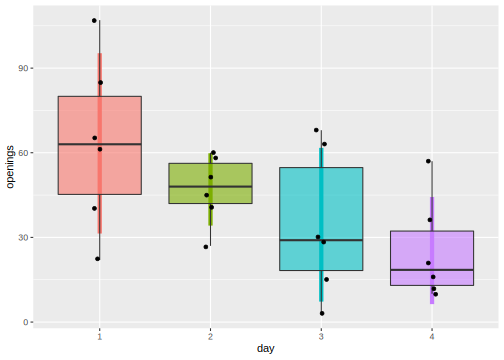
\includegraphics[width=0.7\linewidth]{07-anova_files/figure-latex/anova-plot5-1}

What are our null hypotheses?

\begin{enumerate}
\def\labelenumi{\arabic{enumi}.}
\tightlist
\item
  H0: There is no difference between snakes with respect to the number
  of openings at which they habituate.
\item
  H0: There is no difference between days in terms of the number of
  openings at which the snakes habituate.
\end{enumerate}

Fit the ANOVA model to test these hypotheses:

\begin{Shaded}
\begin{Highlighting}[]
\NormalTok{snakes.aov <-}\StringTok{ }\KeywordTok{aov}\NormalTok{(openings }\OperatorTok{~}\StringTok{ }\NormalTok{day }\OperatorTok{+}\StringTok{ }\NormalTok{snake, }\DataTypeTok{data =}\NormalTok{ snakes)}
\KeywordTok{summary}\NormalTok{(snakes.aov)}
\end{Highlighting}
\end{Shaded}

\begin{verbatim}
R>             Df Sum Sq Mean Sq F value Pr(>F)  
R> day          3   4878  1625.9   3.320 0.0487 *
R> snake        5   3042   608.4   1.242 0.3382  
R> Residuals   15   7346   489.7                 
R> ---
R> Signif. codes:  0 '***' 0.001 '**' 0.01 '*' 0.05 '.' 0.1 ' ' 1
\end{verbatim}

Now we need to test of the assumptions hold true (i.e.~erros are
normally distributed and heteroscedastic). Also, where are the
differences?

\begin{Shaded}
\begin{Highlighting}[]
\KeywordTok{par}\NormalTok{(}\DataTypeTok{mfrow =} \KeywordTok{c}\NormalTok{(}\DecValTok{2}\NormalTok{, }\DecValTok{2}\NormalTok{))}
\CommentTok{# Checking assumptions...}
\CommentTok{# make a histogram of the residuals;}
\CommentTok{# they must be normal}
\NormalTok{snakes.res <-}\StringTok{ }\KeywordTok{residuals}\NormalTok{(snakes.aov)}
\KeywordTok{hist}\NormalTok{(snakes.res, }\DataTypeTok{col =} \StringTok{"red"}\NormalTok{)}

\CommentTok{# make a plot of residuals and the fitted values;}
\CommentTok{# # they must be normal and homoscedastic}
\KeywordTok{plot}\NormalTok{(}\KeywordTok{fitted}\NormalTok{(snakes.aov), }\KeywordTok{residuals}\NormalTok{(snakes.aov), }\DataTypeTok{col =} \StringTok{"red"}\NormalTok{)}

\NormalTok{snakes.tukey <-}\StringTok{ }\KeywordTok{TukeyHSD}\NormalTok{(snakes.aov, }\DataTypeTok{which =} \StringTok{"day"}\NormalTok{, }\DataTypeTok{conf.level =} \FloatTok{0.90}\NormalTok{)}
\KeywordTok{plot}\NormalTok{(snakes.tukey, }\DataTypeTok{las =} \DecValTok{1}\NormalTok{, }\DataTypeTok{col =} \StringTok{"red"}\NormalTok{)}
\end{Highlighting}
\end{Shaded}

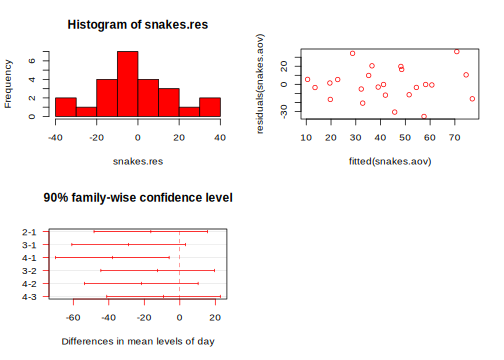
\includegraphics[width=0.7\linewidth]{07-anova_files/figure-latex/anova-plot6-1}

\hypertarget{alternatives-to-anova}{%
\section{Alternatives to ANOVA}\label{alternatives-to-anova}}

In the first main section of this chapter we learned how to test
hypotheses based on the comparisons of means between sets of data when
we were able to meet our two base assumptions. These parametric tests
are preferred over non-parametric tests because they are more robust.
However, when we simply aren't able to meet these assumptions we must
not despair. Non-parametric tests are still useful. In this chapter we
will learn how to run non-parametric tests for two sample and multiple
sample datasets. To start, let's load our libraries and \texttt{chicks}
data if we have not already.

\begin{Shaded}
\begin{Highlighting}[]
\CommentTok{# First activate libraries}
\KeywordTok{library}\NormalTok{(tidyverse)}
\KeywordTok{library}\NormalTok{(ggpubr)}

\CommentTok{# Then load data}
\NormalTok{chicks <-}\StringTok{ }\KeywordTok{as_tibble}\NormalTok{(ChickWeight)}
\end{Highlighting}
\end{Shaded}

With our libraries and data loaded, let's find a day in which at least
one of our assumptions are violated.

\begin{Shaded}
\begin{Highlighting}[]
\CommentTok{# Then check for failing assumptions}
\NormalTok{chicks }\OperatorTok\StringTok{ }
\StringTok{  }\KeywordTok{filter}\NormalTok{(Time }\OperatorTok{==}\StringTok{ }\DecValTok{0}\NormalTok{) }\OperatorTok\StringTok{ }
\StringTok{  }\KeywordTok{group_by}\NormalTok{(Diet) }\OperatorTok\StringTok{ }
\StringTok{  }\KeywordTok{summarise}\NormalTok{(}\DataTypeTok{norm_wt =} \KeywordTok{as.numeric}\NormalTok{(}\KeywordTok{shapiro.test}\NormalTok{(weight)[}\DecValTok{2}\NormalTok{]),}
            \DataTypeTok{var_wt =} \KeywordTok{var}\NormalTok{(weight))}
\end{Highlighting}
\end{Shaded}

\begin{verbatim}
R>       norm_wt   var_wt
R> 1 0.000221918 1.282041
\end{verbatim}

\hypertarget{wilcox-rank-sum-test}{%
\subsection{Wilcox rank sum test}\label{wilcox-rank-sum-test}}

The non-parametric version of a t-test is a Wilcox rank sum test. To
perform this test in R we may again use \texttt{compare\_means()} and
specify the test we want:

\begin{Shaded}
\begin{Highlighting}[]
\KeywordTok{compare_means}\NormalTok{(weight }\OperatorTok{~}\StringTok{ }\NormalTok{Diet, }\DataTypeTok{data =} \KeywordTok{filter}\NormalTok{(chicks, Time }\OperatorTok{==}\StringTok{ }\DecValTok{0}\NormalTok{, Diet }\OperatorTok\StringTok{ }\KeywordTok{c}\NormalTok{(}\DecValTok{1}\NormalTok{, }\DecValTok{2}\NormalTok{)), }\DataTypeTok{method =} \StringTok{"wilcox.test"}\NormalTok{)}
\end{Highlighting}
\end{Shaded}

\begin{verbatim}
R> # A tibble: 1 x 8
R>   .y.    group1 group2     p p.adj p.format p.signif method  
R>   <chr>  <chr>  <chr>  <dbl> <dbl> <chr>    <chr>    <chr>   
R> 1 weight 1      2      0.235 0.235 0.23     ns       Wilcoxon
\end{verbatim}

What do our results show?

\hypertarget{kruskall-wallis-rank-sum-test}{%
\subsection{Kruskall-Wallis rank sum
test}\label{kruskall-wallis-rank-sum-test}}

\hypertarget{single-factor-1}{%
\subsubsection{Single factor}\label{single-factor-1}}

The non-parametric version of an ANOVA is a Kruskall-Wallis rank sum
test. As you may have by now surmised, this may be done with
\texttt{compare\_means()} as seen below:

\begin{Shaded}
\begin{Highlighting}[]
\KeywordTok{compare_means}\NormalTok{(weight }\OperatorTok{~}\StringTok{ }\NormalTok{Diet, }\DataTypeTok{data =} \KeywordTok{filter}\NormalTok{(chicks, Time }\OperatorTok{==}\StringTok{ }\DecValTok{0}\NormalTok{), }\DataTypeTok{method =} \StringTok{"kruskal.test"}\NormalTok{)}
\end{Highlighting}
\end{Shaded}

\begin{verbatim}
R> # A tibble: 1 x 6
R>   .y.        p p.adj p.format p.signif method        
R>   <chr>  <dbl> <dbl> <chr>    <chr>    <chr>         
R> 1 weight 0.475 0.475 0.48     ns       Kruskal-Wallis
\end{verbatim}

As with the ANOVA, this first step with the Kruskall-Wallis test is not
the last. We must again run a post-hoc test on our results. This time we
will need to use \texttt{pgirmess::kruskalmc()}, which means we will
need to load a new library.

\begin{Shaded}
\begin{Highlighting}[]
\KeywordTok{library}\NormalTok{(pgirmess)}

\KeywordTok{kruskalmc}\NormalTok{(weight }\OperatorTok{~}\StringTok{ }\NormalTok{Diet, }\DataTypeTok{data =} \KeywordTok{filter}\NormalTok{(chicks, Time }\OperatorTok{==}\StringTok{ }\DecValTok{0}\NormalTok{))}
\end{Highlighting}
\end{Shaded}

\begin{verbatim}
R> Multiple comparison test after Kruskal-Wallis 
R> p.value: 0.05 
R> Comparisons
R>     obs.dif critical.dif difference
R> 1-2    6.95     14.89506      FALSE
R> 1-3    6.90     14.89506      FALSE
R> 1-4    4.15     14.89506      FALSE
R> 2-3    0.05     17.19933      FALSE
R> 2-4    2.80     17.19933      FALSE
R> 3-4    2.75     17.19933      FALSE
\end{verbatim}

Let's consult the help file for \texttt{kruskalmc()} to understand what
this print-out means.

\hypertarget{multiple-factors-1}{%
\subsubsection{Multiple factors}\label{multiple-factors-1}}

The water becomes murky quickly when one wants to perform multiple
factor non-parametric comparison of means tests. To that end, we will
not cover the few existing methods here. Rather, one should avoid the
necessity for these types of tests when designing an experiment.

\hypertarget{the-sa-time-data}{%
\subsection{The SA time data}\label{the-sa-time-data}}

\begin{Shaded}
\begin{Highlighting}[]
\NormalTok{sa_time <-}\StringTok{ }\KeywordTok{as_tibble}\NormalTok{(}\KeywordTok{read_csv}\NormalTok{(}\StringTok{"data/SA_time.csv"}\NormalTok{, }\DataTypeTok{col_types =} \KeywordTok{list}\NormalTok{(}\KeywordTok{col_double}\NormalTok{(), }\KeywordTok{col_double}\NormalTok{(), }\KeywordTok{col_double}\NormalTok{())))}
\NormalTok{sa_time_long <-}\StringTok{ }\NormalTok{sa_time }\OperatorTok\StringTok{ }
\StringTok{  }\KeywordTok{gather}\NormalTok{(}\DataTypeTok{key =} \StringTok{"term"}\NormalTok{, }\DataTypeTok{value =} \StringTok{"minutes"}\NormalTok{) }\OperatorTok\StringTok{ }
\StringTok{  }\KeywordTok{filter}\NormalTok{(minutes }\OperatorTok{<}\StringTok{ }\DecValTok{300}\NormalTok{) }\OperatorTok\StringTok{ }
\StringTok{  }\KeywordTok{mutate}\NormalTok{(}\DataTypeTok{term =} \KeywordTok{as.factor}\NormalTok{(term))}

\NormalTok{my_comparisons <-}\StringTok{ }\KeywordTok{list}\NormalTok{( }\KeywordTok{c}\NormalTok{(}\StringTok{"now"}\NormalTok{, }\StringTok{"now_now"}\NormalTok{), }\KeywordTok{c}\NormalTok{(}\StringTok{"now_now"}\NormalTok{, }\StringTok{"just_now"}\NormalTok{), }\KeywordTok{c}\NormalTok{(}\StringTok{"now"}\NormalTok{, }\StringTok{"just_now"}\NormalTok{) )}

\KeywordTok{ggboxplot}\NormalTok{(sa_time_long, }\DataTypeTok{x =} \StringTok{"term"}\NormalTok{, }\DataTypeTok{y =} \StringTok{"minutes"}\NormalTok{,}
          \DataTypeTok{color =} \StringTok{"term"}\NormalTok{, }\DataTypeTok{palette =} \KeywordTok{c}\NormalTok{(}\StringTok{"#00AFBB"}\NormalTok{, }\StringTok{"#E7B800"}\NormalTok{, }\StringTok{"#FC4E07"}\NormalTok{),}
          \DataTypeTok{add =} \StringTok{"jitter"}\NormalTok{, }\DataTypeTok{shape =} \StringTok{"term"}\NormalTok{)}
\end{Highlighting}
\end{Shaded}

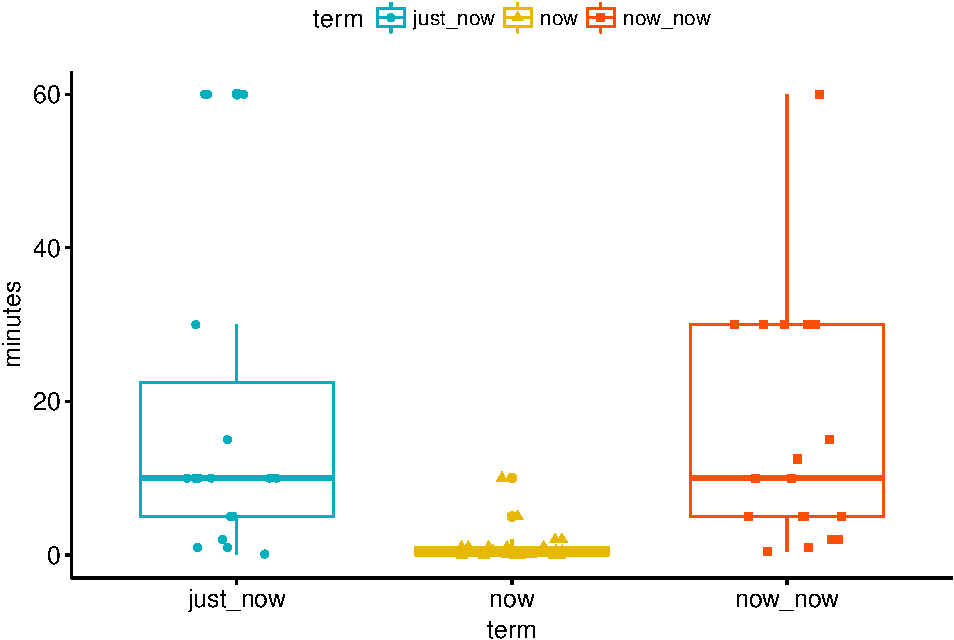
\includegraphics[width=0.7\linewidth]{07-anova_files/figure-latex/anova-plot7-1}

\begin{Shaded}
\begin{Highlighting}[]
\KeywordTok{ggviolin}\NormalTok{(sa_time_long, }\DataTypeTok{x =} \StringTok{"term"}\NormalTok{, }\DataTypeTok{y =} \StringTok{"minutes"}\NormalTok{, }\DataTypeTok{fill =} \StringTok{"term"}\NormalTok{,}
         \DataTypeTok{palette =} \KeywordTok{c}\NormalTok{(}\StringTok{"#00AFBB"}\NormalTok{, }\StringTok{"#E7B800"}\NormalTok{, }\StringTok{"#FC4E07"}\NormalTok{),}
         \DataTypeTok{add =} \StringTok{"boxplot"}\NormalTok{, }\DataTypeTok{add.params =} \KeywordTok{list}\NormalTok{(}\DataTypeTok{fill =} \StringTok{"white"}\NormalTok{)) }\OperatorTok{+}
\StringTok{  }\KeywordTok{stat_compare_means}\NormalTok{(}\DataTypeTok{comparisons =}\NormalTok{ my_comparisons, }\DataTypeTok{label =} \StringTok{"p.signif"}\NormalTok{) }\OperatorTok{+}\StringTok{ }\CommentTok{# Add significance levels}
\StringTok{  }\KeywordTok{stat_compare_means}\NormalTok{(}\DataTypeTok{label.y =} \DecValTok{50}\NormalTok{)                                      }\CommentTok{# Add global the p-value }
\end{Highlighting}
\end{Shaded}

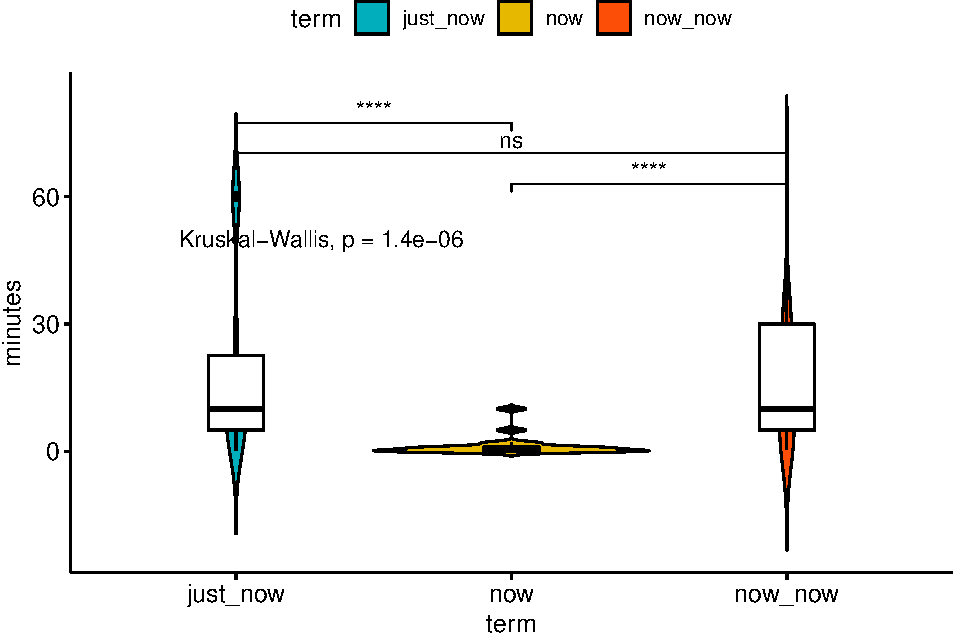
\includegraphics[width=0.7\linewidth]{07-anova_files/figure-latex/anova-plot7-2}

\hypertarget{exercises-4}{%
\section{Exercises}\label{exercises-4}}

\hypertarget{exercise-1-4}{%
\subsection{Exercise 1}\label{exercise-1-4}}

Here is bunch of data for pigs raised on different diets. The experiment
is similar to the chicken one. Does feed type have an effect on the mass
of pigs at the end of the experiment?

\begin{Shaded}
\begin{Highlighting}[]
\CommentTok{# enter the mass at the end of the experiment}
\NormalTok{feed_}\DecValTok{1}\NormalTok{ <-}\StringTok{ }\KeywordTok{c}\NormalTok{(}\FloatTok{60.8}\NormalTok{, }\FloatTok{57.0}\NormalTok{, }\FloatTok{65.0}\NormalTok{, }\FloatTok{58.6}\NormalTok{, }\FloatTok{61.7}\NormalTok{)}
\NormalTok{feed_}\DecValTok{2}\NormalTok{ <-}\StringTok{ }\KeywordTok{c}\NormalTok{(}\FloatTok{68.7}\NormalTok{, }\FloatTok{67.7}\NormalTok{, }\FloatTok{74.0}\NormalTok{, }\FloatTok{66.3}\NormalTok{, }\FloatTok{69.8}\NormalTok{)}
\NormalTok{feed_}\DecValTok{3}\NormalTok{ <-}\StringTok{ }\KeywordTok{c}\NormalTok{(}\FloatTok{102.6}\NormalTok{, }\FloatTok{102.1}\NormalTok{, }\FloatTok{100.2}\NormalTok{, }\FloatTok{96.5}\NormalTok{)}
\NormalTok{feed_}\DecValTok{4}\NormalTok{ <-}\StringTok{ }\KeywordTok{c}\NormalTok{(}\FloatTok{87.9}\NormalTok{, }\FloatTok{84.2}\NormalTok{, }\FloatTok{83.1}\NormalTok{, }\FloatTok{85.7}\NormalTok{, }\FloatTok{90.3}\NormalTok{)}

\CommentTok{# make a dataframe}
\NormalTok{bacon <-}\StringTok{ }\KeywordTok{as.tibble}\NormalTok{(}\KeywordTok{data.frame}\NormalTok{(}
  \DataTypeTok{feed =} \KeywordTok{c}\NormalTok{(}
  \KeywordTok{rep}\NormalTok{(}\StringTok{"Feed 1"}\NormalTok{, }\KeywordTok{length}\NormalTok{(feed_}\DecValTok{1}\NormalTok{)),}
  \KeywordTok{rep}\NormalTok{(}\StringTok{"Feed 2"}\NormalTok{, }\KeywordTok{length}\NormalTok{(feed_}\DecValTok{2}\NormalTok{)),}
  \KeywordTok{rep}\NormalTok{(}\StringTok{"Feed 3"}\NormalTok{, }\KeywordTok{length}\NormalTok{(feed_}\DecValTok{3}\NormalTok{)),}
  \KeywordTok{rep}\NormalTok{(}\StringTok{"Feed 4"}\NormalTok{, }\KeywordTok{length}\NormalTok{(feed_}\DecValTok{4}\NormalTok{))}
\NormalTok{  ),}
  \DataTypeTok{mass =} \KeywordTok{c}\NormalTok{(feed_}\DecValTok{1}\NormalTok{, feed_}\DecValTok{2}\NormalTok{, feed_}\DecValTok{3}\NormalTok{, feed_}\DecValTok{4}\NormalTok{)}
\NormalTok{  ))}
\end{Highlighting}
\end{Shaded}

\hypertarget{exercise-2-1}{%
\subsection{Exercise 2}\label{exercise-2-1}}

Construct suitable null and alternative hypotheses for the built-in
\texttt{ToothGrowth} data, and test your hypotheses using an ANOVA.

\begin{Shaded}
\begin{Highlighting}[]
\NormalTok{teeth <-}\StringTok{ }\NormalTok{datasets}\OperatorTok{::}\NormalTok{ToothGrowth}
\end{Highlighting}
\end{Shaded}

\hypertarget{exercise-3}{%
\subsection{Exercise 3}\label{exercise-3}}

Find or generate your own data that lend themselves to being analysed by
a two-way ANOVA. Generate suitable hypotheses about your data, and
analyse it. Supplement your analysis by providing a suitable descriptive
statistical summary and graph(s) of your data.

\hypertarget{simple-linear-regressions}{%
\chapter{Simple linear regressions}\label{simple-linear-regressions}}

\begin{Shaded}
\begin{Highlighting}[]
\KeywordTok{library}\NormalTok{(tidyverse)}
\end{Highlighting}
\end{Shaded}

Regressions test the statistical significance of the \emph{dependence}
of one continuous variable on one or many independent continuous
variables.

\hypertarget{the-simple-linear-regression-equation}{%
\section{The simple linear regression
equation}\label{the-simple-linear-regression-equation}}

The linear regression equation is already known to you. It is:

\[y_{n}=\beta \cdot x_{n}+\alpha+\epsilon\]

Coefficients are parameters (statistics) that describe two properties of
the linear line that best fit a scatter plot between a dependent
variable and the independent variable. The dependent variable,
\(y_{1..n}\), may also be called the response variable, and the
independent variable, \(x_{1..n}\), the predictor. The regression model
consists of an \emph{intercept term}, \(\alpha\), that describes where
the fitted line starts and intercepts with the \emph{y}-axis, and the
\emph{slope}, \(\beta\), of the line. The amount of variation not
explained by a linear relationship of \(y\) on \(x\) is termed the
residual variation, or simply the residual or the error term, and in the
above equation it is indicated by \(\epsilon\).

The regression parameters \(\alpha\) and \(\beta\) are determined by
\emph{minimising the error sum of squares} of the error term,
\(\epsilon\). It allows us to predict new fitted values of \(y\) based
on values of \(x\). The error sum of squares is calculated by:

\[error~SS=\sum_{i=1}^{n}(y_{i}-\hat{y}_{i})^{2}\]

To see an animation demonstrating this click
\href{https://raw.githubusercontent.com/ajsmit/Basic_stats/master/figures/lm_rotate.avi}{here}.

We will demonstrate the principle behind a simple linear regression by
using the built-in dataset \texttt{faithful}. According to the R help
file for the data, the dataset describes the \enquote{Waiting time
between eruptions and the duration of the eruption for the Old Faithful
geyser in Yellowstone National Park, Wyoming, USA.}

\begin{Shaded}
\begin{Highlighting}[]
\KeywordTok{head}\NormalTok{(faithful)}
\end{Highlighting}
\end{Shaded}

\begin{verbatim}
R>   eruptions waiting
R> 1     3.600      79
R> 2     1.800      54
R> 3     3.333      74
R> 4     2.283      62
R> 5     4.533      85
R> 6     2.883      55
\end{verbatim}

In this dataset there are two columns: the first, \texttt{eruptions},
denotes the duration of the eruption (in minutes), and the second,
\texttt{waiting}, is the waiting time (also in minutes) until the next
eruptions. Its linear regression model can be expressed as:

\[eruption_{n}=\beta \cdot waiting_{n}+\alpha+\epsilon\]

Here we fit the model in R. When we perform a linear regression in R, it
will output the model and the coefficients:

\begin{Shaded}
\begin{Highlighting}[]
\NormalTok{eruption.lm <-}\StringTok{ }\KeywordTok{lm}\NormalTok{(eruptions }\OperatorTok{~}\StringTok{ }\NormalTok{waiting, }\DataTypeTok{data =}\NormalTok{ faithful)}
\KeywordTok{summary}\NormalTok{(eruption.lm)}
\end{Highlighting}
\end{Shaded}

\begin{verbatim}
R> 
R> Call:
R> lm(formula = eruptions ~ waiting, data = faithful)
R> 
R> Residuals:
R>      Min       1Q   Median       3Q      Max 
R> -1.29917 -0.37689  0.03508  0.34909  1.19329 
R> 
R> Coefficients:
R>              Estimate Std. Error t value Pr(>|t|)    
R> (Intercept) -1.874016   0.160143  -11.70   <2e-16 ***
R> waiting      0.075628   0.002219   34.09   <2e-16 ***
R> ---
R> Signif. codes:  0 '***' 0.001 '**' 0.01 '*' 0.05 '.' 0.1 ' ' 1
R> 
R> Residual standard error: 0.4965 on 270 degrees of freedom
R> Multiple R-squared:  0.8115, Adjusted R-squared:  0.8108 
R> F-statistic:  1162 on 1 and 270 DF,  p-value: < 2.2e-16
\end{verbatim}

\hypertarget{the-intercept}{%
\subsection{The intercept}\label{the-intercept}}

The intercept is the best estimate of the starting point of the fitted
line on the lefthand side of the graph. You will notice that there is
also an estimate for the standard error of the estimate for the
intercept.

\hypertarget{the-regression-coefficient}{%
\subsection{The regression
coefficient}\label{the-regression-coefficient}}

The interpretation of the regression coefficient is simple. For every
one unit of change in the independent variable (here waiting time) there
is a corresponding change in the dependent variable (here the duration
of the eruption). This is the \emph{slope} or \emph{gradient}, and it
may be positive or negative. In the example the coefficient of
determination of the line is denoted by the value 0.076
min.min\textsuperscript{-1} in the column termed \texttt{Estimate} and
in the row called \texttt{waiting} (the latter name will of course
depend on the name of the response column in your dataset). The
coefficient of determination multiplies the response variable to produce
a prediction of the response based on the slope of the relationship
between the response and the predictor. It tells us how much one unit in
change of the independent variable \emph{determines} the corresponding
change in the response variable. There is also a standard error for the
estimate.

\hypertarget{a-graph-of-the-linear-regression}{%
\subsection{A graph of the linear
regression}\label{a-graph-of-the-linear-regression}}

\begin{Shaded}
\begin{Highlighting}[]
\NormalTok{slope <-}\StringTok{ }\KeywordTok{round}\NormalTok{(eruption.lm}\OperatorTok{$}\NormalTok{coef[}\DecValTok{2}\NormalTok{], }\DecValTok{3}\NormalTok{)}
\CommentTok{# p.val <- round(coefficients(summary(eruption.lm))[2, 4], 3) # it approx. 0, so...}
\NormalTok{p.val =}\StringTok{ }\FloatTok{0.001}
\NormalTok{r2 <-}\StringTok{ }\KeywordTok{round}\NormalTok{(}\KeywordTok{summary}\NormalTok{(eruption.lm)}\OperatorTok{$}\NormalTok{r.squared, }\DecValTok{3}\NormalTok{)}

\KeywordTok{ggplot}\NormalTok{(}\DataTypeTok{data =}\NormalTok{ faithful, }\KeywordTok{aes}\NormalTok{(}\DataTypeTok{x =}\NormalTok{ waiting, }\DataTypeTok{y =}\NormalTok{ eruptions)) }\OperatorTok{+}
\StringTok{  }\KeywordTok{geom_point}\NormalTok{() }\OperatorTok{+}
\StringTok{  }\KeywordTok{annotate}\NormalTok{(}\StringTok{"text"}\NormalTok{, }\DataTypeTok{x =} \DecValTok{45}\NormalTok{, }\DataTypeTok{y =} \DecValTok{5}\NormalTok{, }\DataTypeTok{label =} \KeywordTok{paste0}\NormalTok{(}\StringTok{"slope == "}\NormalTok{, slope, }\StringTok{"~(min/min)"}\NormalTok{), }\DataTypeTok{parse =} \OtherTok{TRUE}\NormalTok{, }\DataTypeTok{hjust =} \DecValTok{0}\NormalTok{) }\OperatorTok{+}
\StringTok{  }\KeywordTok{annotate}\NormalTok{(}\StringTok{"text"}\NormalTok{, }\DataTypeTok{x =} \DecValTok{45}\NormalTok{, }\DataTypeTok{y =} \FloatTok{4.75}\NormalTok{, }\DataTypeTok{label =} \KeywordTok{paste0}\NormalTok{(}\StringTok{"italic(p) < "}\NormalTok{, p.val), }\DataTypeTok{parse =} \OtherTok{TRUE}\NormalTok{, }\DataTypeTok{hjust =} \DecValTok{0}\NormalTok{) }\OperatorTok{+}
\StringTok{  }\KeywordTok{annotate}\NormalTok{(}\StringTok{"text"}\NormalTok{, }\DataTypeTok{x =} \DecValTok{45}\NormalTok{, }\DataTypeTok{y =} \FloatTok{4.5}\NormalTok{, }\DataTypeTok{label =} \KeywordTok{paste0}\NormalTok{(}\StringTok{"italic(r)^2 == "}\NormalTok{, r2), }\DataTypeTok{parse =} \OtherTok{TRUE}\NormalTok{, }\DataTypeTok{hjust =} \DecValTok{0}\NormalTok{) }\OperatorTok{+}
\StringTok{  }\KeywordTok{stat_smooth}\NormalTok{(}\DataTypeTok{method =} \StringTok{"lm"}\NormalTok{, }\DataTypeTok{colour =} \StringTok{"salmon"}\NormalTok{) }\OperatorTok{+}
\StringTok{  }\KeywordTok{labs}\NormalTok{(}\DataTypeTok{title =} \StringTok{"Old Faithful eruption data"}\NormalTok{,}
       \DataTypeTok{subtitle =} \StringTok{"Linear regression"}\NormalTok{,}
       \DataTypeTok{x =} \StringTok{"Waiting time (minutes)"}\NormalTok{,}
       \DataTypeTok{y =} \StringTok{"Eruption duration (minutes)"}\NormalTok{)}
\end{Highlighting}
\end{Shaded}

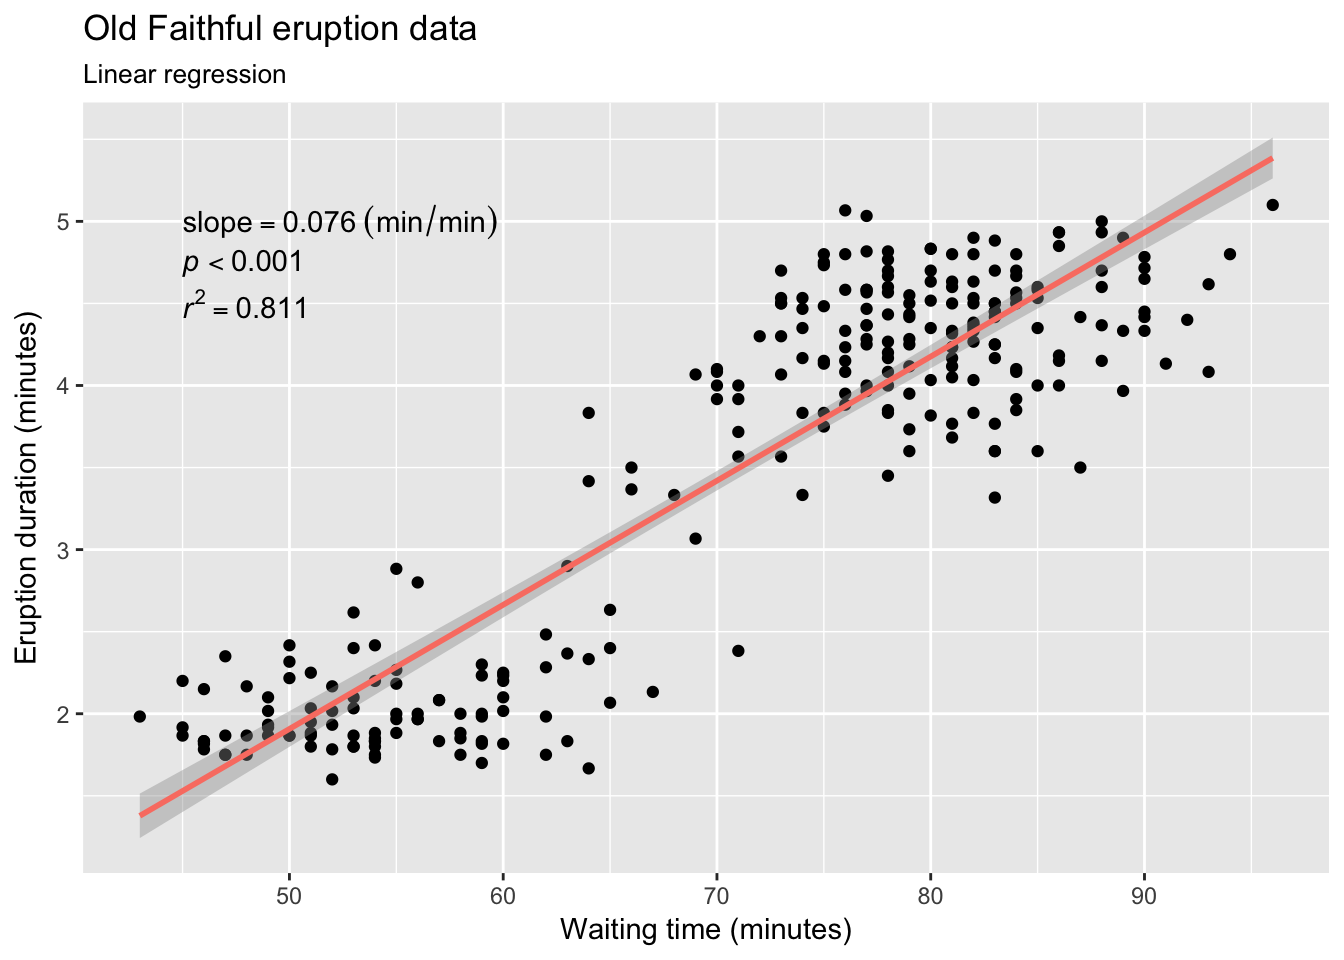
\includegraphics[width=0.7\linewidth]{08-regressions_files/figure-latex/lm-plot1-1}

\hypertarget{predicting-from-the-linear-model}{%
\subsection{Predicting from the linear
model}\label{predicting-from-the-linear-model}}

Knowing \(\alpha\) and \(\beta\) allows us to predict what the eruption
duration will be for a certain amount of waiting. Since the slope of the
line is positive we can expect that the longer the waiting time is
between eruptions the longer the eruption would be. But how can we
quantify this? We start by extracting the coefficients (both the
intercept and the regression coefficient). Then we use these values to
reassemble the regression equation that we have written out above (i.e.,
\(eruption_{n}=\beta \cdot waiting_{n}+\alpha+\epsilon\)). Here's how:

\begin{Shaded}
\begin{Highlighting}[]
\CommentTok{# use the accessor function to grab the coefficients:}
\NormalTok{erupt.coef <-}\StringTok{ }\KeywordTok{coefficients}\NormalTok{(eruption.lm)}
\NormalTok{erupt.coef}
\end{Highlighting}
\end{Shaded}

\begin{verbatim}
R> (Intercept)     waiting 
R> -1.87401599  0.07562795
\end{verbatim}

\begin{Shaded}
\begin{Highlighting}[]
\CommentTok{# how long would an eruption last of we waited, say, 80 minutes?}
\NormalTok{waiting <-}\StringTok{ }\DecValTok{80} 
 
\CommentTok{# the first and second coef. can be accessed using the }
\CommentTok{# square bracket notation:}
\NormalTok{erupt.pred <-}\StringTok{ }\NormalTok{erupt.coef[}\DecValTok{1}\NormalTok{] }\OperatorTok{+}\StringTok{ }\NormalTok{(erupt.coef[}\DecValTok{2}\NormalTok{] }\OperatorTok{*}\StringTok{ }\NormalTok{waiting)}
\NormalTok{erupt.pred }\CommentTok{# the unit is minutes}
\end{Highlighting}
\end{Shaded}

\begin{verbatim}
R> (Intercept) 
R>     4.17622
\end{verbatim}

The prediction is that, given a waiting time of 80 minutes since the
previous eruption, the next eruption will last 4.176 minutes.

There is another way to do this. The \texttt{predict()} function takes a
dataframe of values for which we want to predict the duration of the
eruption and returns a vector with the waiting times:

\begin{Shaded}
\begin{Highlighting}[]
\NormalTok{pred.val <-}\StringTok{ }\KeywordTok{data.frame}\NormalTok{(}\DataTypeTok{waiting =} \KeywordTok{c}\NormalTok{(}\DecValTok{60}\NormalTok{, }\DecValTok{80}\NormalTok{, }\DecValTok{100}\NormalTok{))}
\KeywordTok{predict}\NormalTok{(eruption.lm, pred.val) }\CommentTok{# returns waiting time in minutes}
\end{Highlighting}
\end{Shaded}

\begin{verbatim}
R>        1        2        3 
R> 2.663661 4.176220 5.688779
\end{verbatim}

\hypertarget{the-coefficient-of-determination-r2}{%
\subsection{\texorpdfstring{The coefficient of determination,
\(r^{2}\)}{The coefficient of determination, r\^{}\{2\}}}\label{the-coefficient-of-determination-r2}}

The coefficient of determination, the \(r^{2}\), of a linear model is
the quotient of the variances of the fitted values, \(\hat{y_{i}}\), and
observed values, \(y_{i}\), of the dependent variable. If the mean of
the dependent variable is \(\bar y\), then the \(r^{2}\) is:

\[r^{2}=\frac{\sum(\hat{y_{i}} - \bar{y})^{2}}{\sum(y_{i} - \bar{y})^{2}}\]

In our Old Faithful example, the coefficient of determination is
returned together with the summary of the \texttt{eruption.lm} object,
but it may also be extracted as:

\begin{Shaded}
\begin{Highlighting}[]
\KeywordTok{summary}\NormalTok{(eruption.lm)}\OperatorTok{$}\NormalTok{r.squared}
\end{Highlighting}
\end{Shaded}

\begin{verbatim}
R> [1] 0.8114608
\end{verbatim}

What does the \(r^{2}\) tell us? It tells us the \enquote{fraction of
variance explained by the model} (from the \texttt{summary.lm()} help
file). In other words it is the proportion of variation in the
dispersion (variance) of the measured dependent variable, \(y\), that
can be predicted from the measured independent variable, \(x\) (or
variables in the case of multiple regressions). It gives us an
indication of how well the observed outcome variable is predicted by the
observed influential variable, and in the case of a simple linear
regression, the geometric relationship of \(y\) on \(x\) is a straight
line. \(r^{2}\) can take values from 0 to 1: a value of 0 tells us that
there is absolutely no relationship between the two, whilst a value of 1
shows that there is a perfect fit and a scatter of points to denote the
\(y\) vs. \(x\) relationship will all fall perfectly on a straight line.

\begin{Shaded}
\begin{Highlighting}[]
\KeywordTok{library}\NormalTok{(tidyverse)}
\NormalTok{n <-}\StringTok{ }\DecValTok{100}
\KeywordTok{set.seed}\NormalTok{(}\DecValTok{666}\NormalTok{)}
\NormalTok{rand.df <-}\StringTok{ }\KeywordTok{data.frame}\NormalTok{(}\DataTypeTok{x =} \KeywordTok{seq}\NormalTok{(}\DecValTok{1}\OperatorTok{:}\NormalTok{n),}
                      \DataTypeTok{y =} \KeywordTok{rnorm}\NormalTok{(}\DataTypeTok{n =}\NormalTok{ n, }\DataTypeTok{mean =} \DecValTok{20}\NormalTok{, }\DataTypeTok{sd =} \DecValTok{3}\NormalTok{))}
\KeywordTok{ggplot}\NormalTok{(}\DataTypeTok{data =}\NormalTok{ rand.df, }\KeywordTok{aes}\NormalTok{(}\DataTypeTok{x =}\NormalTok{ x, }\DataTypeTok{y =}\NormalTok{ y)) }\OperatorTok{+}
\StringTok{  }\KeywordTok{geom_point}\NormalTok{(}\DataTypeTok{colour =} \StringTok{"blue"}\NormalTok{) }\OperatorTok{+}
\StringTok{  }\KeywordTok{stat_smooth}\NormalTok{(}\DataTypeTok{method =} \StringTok{"lm"}\NormalTok{, }\DataTypeTok{colour =} \StringTok{"purple"}\NormalTok{, }\DataTypeTok{size =} \FloatTok{0.75}\NormalTok{, }\DataTypeTok{fill =} \StringTok{"turquoise"}\NormalTok{, }\DataTypeTok{alpha =} \FloatTok{0.3}\NormalTok{) }\OperatorTok{+}
\StringTok{  }\KeywordTok{labs}\NormalTok{(}\DataTypeTok{title =} \StringTok{"Random normal data"}\NormalTok{,}
       \DataTypeTok{subtitle =} \StringTok{"Linear regression"}\NormalTok{,}
       \DataTypeTok{x =} \StringTok{"X (independent variable)"}\NormalTok{,}
       \DataTypeTok{y =} \StringTok{"Y (dependent variable)"}\NormalTok{)}
\end{Highlighting}
\end{Shaded}

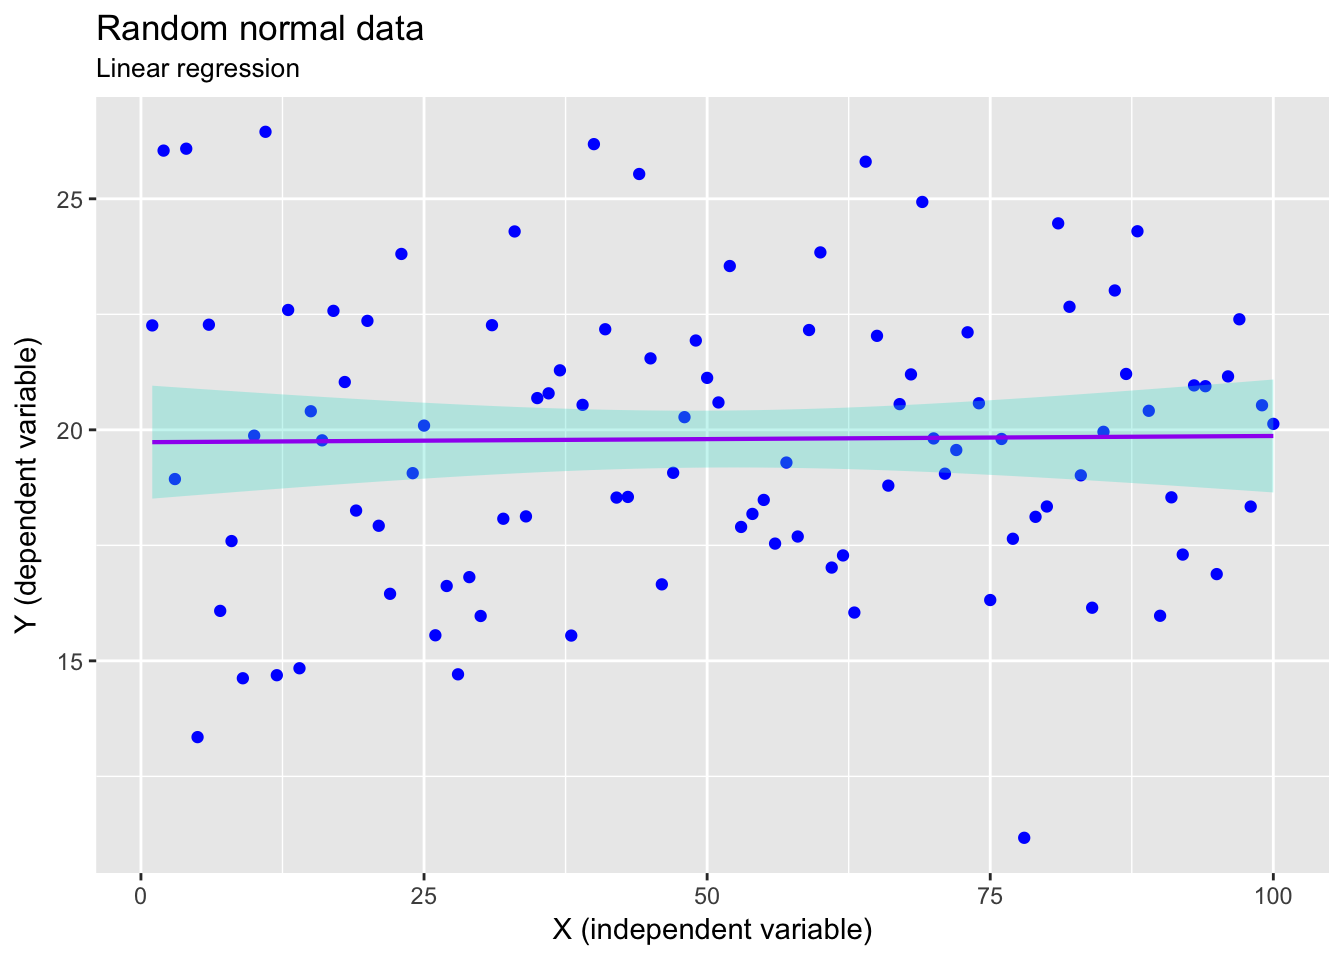
\includegraphics[width=0.7\linewidth]{08-regressions_files/figure-latex/lm-plot2-1}

Regressions may take on any relationship, not only a linear one. For
example, there are parabolic, hyperbolic, logistic, exponential, etc.
relationships of \(y\) on \(x\), and here, too, does \(r^{2}\) tell us
the same thing. If we assume that the samples were representatively
drawn from a population (i.e.~the sample fully captures the relationship
of \(y\) on \(x\) that is present in the entire population), the
\(r^{2}\) will represent the relationship in the population too.

In the case of our Old Faithful data, the \(r^{2}\) is 0.811, meaning
that the proportion of variance explained is 81.1\%; the remaining
18.9\% is not (yet) accounted for by the linear relationship. Adding
more predictors into the regression (i.e.~a multiple regression) might
consume some of the unexplained variance and increase the overall
\(r^{2}\).

\hypertarget{significance-test-for-linear-regression}{%
\subsection{Significance test for linear
regression}\label{significance-test-for-linear-regression}}

There are several hypothesis tests associated with a simple linear
regression. All of them assume that the residual error, \(\epsilon\), in
the linear regression model is independent of \(x\) (i.e.~nothing about
the structure of the error term can be inferred based on a knowledge of
\(x\)), is normally distributed, with zero mean and constant variance.
We say the residuals are \emph{i.i.d.} (independent and identically
distributed, which is a fancy way of saying they are random).

We can decide whether there is any significant relationship (slope) of
\(y\) on \(x\) by testing the null hypothesis that \(\beta=0\).
Rejecting the null hypothesis causes the alternate hypothesis of
\(\beta \neq 0\) to be accepted. This test is automatically performed
when fitting a linear model in R and asking for a summary of the
regression object, but it is insightful and important to know that the
test is simply a one-sample \emph{t}-test. In the regression summary the
probability associated with this test is given in the
\texttt{Coefficients} table in the column called
\texttt{Pr(\textgreater{}\textbar{}t\textbar{})}.

In the Old Faithful data, the \emph{p}-value associated with
\texttt{waiting} is less than 0.05 and we therefore reject the null
hypothesis that \(\beta=0\). So, there is a significant linear
relationship of eruption duration on the waiting time between eruptions.

\begin{quote}
\textbf{Question:} Note that there is also a hypothesis test in the
\texttt{(Intercept)} row. What does this do?
\end{quote}

\hypertarget{confidence-interval-for-linear-regression}{%
\subsection{Confidence interval for linear
regression}\label{confidence-interval-for-linear-regression}}

Again we have to observe the assumption of \emph{i.i.d.} as before. For
a given value of \(x\), the 95\% confidence interval around the mean of
the \emph{observed} dependent variable, \(\bar{y}\), can be obtained as
follows:

\begin{Shaded}
\begin{Highlighting}[]
\NormalTok{pred.val <-}\StringTok{ }\KeywordTok{data.frame}\NormalTok{(}\DataTypeTok{waiting =} \KeywordTok{c}\NormalTok{(}\DecValTok{80}\NormalTok{))}
\KeywordTok{predict}\NormalTok{(eruption.lm, pred.val, }\DataTypeTok{interval =} \StringTok{"confidence"}\NormalTok{)}
\end{Highlighting}
\end{Shaded}

\begin{verbatim}
R>       fit      lwr      upr
R> 1 4.17622 4.104848 4.247592
\end{verbatim}

So, the 95\% confidence interval of the mean eruption duration for the
waiting time of 80 minutes is between 4.105 and 4.248 minutes.

\hypertarget{prediction-interval-for-linear-regression}{%
\subsection{Prediction interval for linear
regression}\label{prediction-interval-for-linear-regression}}

Observe that \(\epsilon\) is \emph{i.i.d.} For a given value of \(x\),
the interval estimate of the \emph{future} dependent variable, \(y\), is
called the prediction interval. The way we do this is similar to finding
the confidence interval:

\begin{Shaded}
\begin{Highlighting}[]
\NormalTok{pred.val <-}\StringTok{ }\KeywordTok{data.frame}\NormalTok{(}\DataTypeTok{waiting =} \KeywordTok{c}\NormalTok{(}\DecValTok{80}\NormalTok{))}
\KeywordTok{predict}\NormalTok{(eruption.lm, pred.val, }\DataTypeTok{interval =} \StringTok{"prediction"}\NormalTok{)}
\end{Highlighting}
\end{Shaded}

\begin{verbatim}
R>       fit      lwr      upr
R> 1 4.17622 3.196089 5.156351
\end{verbatim}

The intervals are wider. The difference between confidence and
prediction intervals is subtle and requires some philosophical
consideration. In practice, if you use these intervals to make
inferences about the population from which the samples were drawn, use
the prediction intervals. If you instead want to describe the samples
which you have taken, use the confidence intervals.

\hypertarget{residual-plot}{%
\subsection{Residual plot}\label{residual-plot}}

\hypertarget{standardised-residual}{%
\subsection{Standardised residual}\label{standardised-residual}}

\hypertarget{normal-probability-plot-of-residuals}{%
\subsection{Normal probability plot of
residuals}\label{normal-probability-plot-of-residuals}}

\hypertarget{using-an-additional-categorical-variable}{%
\section{Using an additional categorical
variable}\label{using-an-additional-categorical-variable}}

\begin{itemize}
\tightlist
\item
  When you use a categorical variable, in R the intercept represents the
  default position for a given value in the categorical column. Every
  other value then gets a modifier to the base prediction.
\end{itemize}

\hypertarget{correlations}{%
\chapter{Correlations}\label{correlations}}

A correlation is performed when we want to investigate potential
relationships between variables from the same sample. This does not mean
that one variable explains the other, we arrive at that through the use
of regression, as seen in Chapter 8. Like all statistical tests,
correlation requires a series of assumptions as well:

\begin{itemize}
\tightlist
\item
  pair-wise data
\item
  absence of outliers
\item
  linearity
\item
  normality of distribution
\item
  homoscedasticity
\item
  level (type) of measurement

  \begin{itemize}
  \tightlist
  \item
    Continuous data (Pearson correlation)
  \item
    Ordinal data (Spearman correlation)
  \end{itemize}
\end{itemize}

In order to investigate correlations in biological data lets load the
\texttt{ecklonia} dataset.

\begin{Shaded}
\begin{Highlighting}[]
\CommentTok{# Load libraries}
\KeywordTok{library}\NormalTok{(tidyverse)}
\KeywordTok{library}\NormalTok{(ggpubr)}
\KeywordTok{library}\NormalTok{(corrplot)}

\CommentTok{# Load data}
\NormalTok{ecklonia <-}\StringTok{ }\KeywordTok{read_csv}\NormalTok{(}\StringTok{"data/ecklonia.csv"}\NormalTok{)}
\end{Highlighting}
\end{Shaded}

We will also create a subsetted version of our data by removing all of
the categorical variables. If we have a dataframe where each column
represents pair-wise continuous/ordinal measurements with all of the
other columns we may very quickly and easily perform a much wider range
of correlation analyses.

\begin{Shaded}
\begin{Highlighting}[]
\NormalTok{ecklonia_sub <-}\StringTok{ }\NormalTok{ecklonia }\OperatorTok\StringTok{ }
\StringTok{  }\KeywordTok{select}\NormalTok{(}\OperatorTok{-}\NormalTok{species, }\OperatorTok{-}\StringTok{ }\NormalTok{site, }\OperatorTok{-}\StringTok{ }\NormalTok{ID)}
\end{Highlighting}
\end{Shaded}

\hypertarget{pearson-correlation}{%
\section{Pearson correlation}\label{pearson-correlation}}

When the values we are comparing are continuous, we may use a Pearson
test. This is the default and so requires little work on our end. The
resulting statistic from this test is known as the correlation
coefficient.

\begin{Shaded}
\begin{Highlighting}[]
\CommentTok{# Perform correlation analysis on two specific variables}
  \CommentTok{# Note that we do not need the final two arguments in this function to be stated}
  \CommentTok{# as they are the defaut settings.}
  \CommentTok{# They are only shown here to illustrate that they exist.}
\KeywordTok{cor.test}\NormalTok{(}\DataTypeTok{x =}\NormalTok{ ecklonia}\OperatorTok{$}\NormalTok{stipe_length, ecklonia}\OperatorTok{$}\NormalTok{frond_length,}
    \DataTypeTok{use =} \StringTok{"everything"}\NormalTok{, }\DataTypeTok{method =} \StringTok{"pearson"}\NormalTok{)}
\end{Highlighting}
\end{Shaded}

\begin{verbatim}
R> 
R>  Pearson's product-moment correlation
R> 
R> data:  ecklonia$stipe_length and ecklonia$frond_length
R> t = 4.2182, df = 24, p-value = 0.0003032
R> alternative hypothesis: true correlation is not equal to 0
R> 95 percent confidence interval:
R>  0.3548169 0.8300525
R> sample estimates:
R>       cor 
R> 0.6524911
\end{verbatim}

Above we have tested the correlation between the length of
\emph{Ecklonia maxima} stipes and the length of their fronds. A perfect
positive (negative) relationship would produce a value of 1 (-1),
whereas no relationship would produce a value of 0. The result above,
\texttt{cor\ =\ 0.65} is relatively strong. That being said, should our
dataset contain multiple variables, as \texttt{ecklonia} does, we may
investigate all of the correlations simultaneously. Remember that in
order to do so we want to ensure that we may perform the same test on
each of our paired variables. In this case we will use
\texttt{ecklonia\_sub} as we know that it contains only continuous data
and so are appropriate for use with a Pearson test. By default R will
use all of the data we give it and perform a Pearson test so we do not
need to specify any further arguments. Note however that this will only
output the correlation coefficients, and does not produce a full test of
each correlation. This will however be useful for us to have just now.

\begin{Shaded}
\begin{Highlighting}[]
\NormalTok{ecklonia_pearson <-}\StringTok{ }\KeywordTok{cor}\NormalTok{(ecklonia_sub)}
\NormalTok{ecklonia_pearson}
\end{Highlighting}
\end{Shaded}

\begin{verbatim}
R>                      stipe_length stipe_diameter frond_length     digits
R> stipe_length            1.0000000      0.5853577   0.65249111 0.24273818
R> stipe_diameter          0.5853577      1.0000000   0.39032107 0.24098021
R> frond_length            0.6524911      0.3903211   1.00000000 0.35604257
R> digits                  0.2427382      0.2409802   0.35604257 1.00000000
R> primary_blade_width     0.3413692      0.8269196   0.28307223 0.13954003
R> primary_blade_length    0.1330329      0.3176688  -0.01584175 0.09784266
R> stipe_mass              0.5768102      0.8226091   0.39471926 0.06958775
R> frond_mass              0.5124551      0.5066763   0.56762418 0.28162375
R> epiphyte_length         0.6056152      0.5372470   0.61489806 0.04634642
R>                      primary_blade_width primary_blade_length stipe_mass
R> stipe_length                   0.3413692           0.13303292 0.57681018
R> stipe_diameter                 0.8269196           0.31766879 0.82260910
R> frond_length                   0.2830722          -0.01584175 0.39471926
R> digits                         0.1395400           0.09784266 0.06958775
R> primary_blade_width            1.0000000           0.33931061 0.82745162
R> primary_blade_length           0.3393106           1.00000000 0.16175948
R> stipe_mass                     0.8274516           0.16175948 1.00000000
R> frond_mass                     0.3630630           0.14729132 0.47195130
R> epiphyte_length                0.4119969           0.26051399 0.50790877
R>                      frond_mass epiphyte_length
R> stipe_length          0.5124551      0.60561520
R> stipe_diameter        0.5066763      0.53724704
R> frond_length          0.5676242      0.61489806
R> digits                0.2816237      0.04634642
R> primary_blade_width   0.3630630      0.41199691
R> primary_blade_length  0.1472913      0.26051399
R> stipe_mass            0.4719513      0.50790877
R> frond_mass            1.0000000      0.43920289
R> epiphyte_length       0.4392029      1.00000000
\end{verbatim}

\begin{quote}
\textbf{Task:} What does the outcome of this test show?
\end{quote}

\hypertarget{spearman-rank-correlation}{%
\section{Spearman rank correlation}\label{spearman-rank-correlation}}

When the data we want to compare are not continuous, but rather ordinal,
we will need to use a Spearman test. This is not often a test one uses
in biology because we tend to want to compare continuous data within
categories. In the code below we will add a column of ordinal data to
our \texttt{ecklonia} data to so that we may look at this test.

\begin{Shaded}
\begin{Highlighting}[]
\CommentTok{# Create ordinal data}
\NormalTok{ecklonia}\OperatorTok{$}\NormalTok{length <-}\StringTok{ }\KeywordTok{as.numeric}\NormalTok{(}\KeywordTok{cut}\NormalTok{((ecklonia}\OperatorTok{$}\NormalTok{stipe_length}\OperatorTok{+}\NormalTok{ecklonia}\OperatorTok{$}\NormalTok{frond_length), }\DataTypeTok{breaks =} \DecValTok{3}\NormalTok{))}

\CommentTok{# Run test on any variable}
\KeywordTok{cor.test}\NormalTok{(ecklonia}\OperatorTok{$}\NormalTok{length, ecklonia}\OperatorTok{$}\NormalTok{digits)}
\end{Highlighting}
\end{Shaded}

\begin{verbatim}
R> 
R>  Pearson's product-moment correlation
R> 
R> data:  ecklonia$length and ecklonia$digits
R> t = 1.4979, df = 24, p-value = 0.1472
R> alternative hypothesis: true correlation is not equal to 0
R> 95 percent confidence interval:
R>  -0.1070908  0.6105880
R> sample estimates:
R>     cor 
R> 0.29239
\end{verbatim}

\begin{quote}
\textbf{Task:} How else might we use this?
\end{quote}

\hypertarget{kendall-rank-correlation}{%
\section{Kendall rank correlation}\label{kendall-rank-correlation}}

This test will work for both continuous and ordinal data. A sort of
dealers choice of correlation tests. It's main purpose is to allow us to
perform a correlation on non-normally distributed data. Let's look at
the normality of our \texttt{ecklonia} variables and pull out those that
are not normal in order to see how the results of this test may differ
from our Pearson tests.

\begin{Shaded}
\begin{Highlighting}[]
\NormalTok{ecklonia_norm <-}\StringTok{ }\NormalTok{ecklonia_sub }\OperatorTok\StringTok{ }
\StringTok{  }\KeywordTok{gather}\NormalTok{(}\DataTypeTok{key =} \StringTok{"variable"}\NormalTok{) }\OperatorTok\StringTok{ }
\StringTok{  }\KeywordTok{group_by}\NormalTok{(variable) }\OperatorTok\StringTok{ }
\StringTok{  }\KeywordTok{summarise}\NormalTok{(}\DataTypeTok{variable_norm =} \KeywordTok{as.numeric}\NormalTok{(}\KeywordTok{shapiro.test}\NormalTok{(value)[}\DecValTok{2}\NormalTok{]))}
\NormalTok{ecklonia_norm}
\end{Highlighting}
\end{Shaded}

\begin{verbatim}
R> # A tibble: 9 x 2
R>   variable             variable_norm
R>   <chr>                        <dbl>
R> 1 digits                     0.0671 
R> 2 epiphyte_length            0.626  
R> 3 frond_length               0.202  
R> 4 frond_mass                 0.277  
R> 5 primary_blade_length       0.00393
R> 6 primary_blade_width        0.314  
R> 7 stipe_diameter             0.170  
R> 8 stipe_length               0.213  
R> 9 stipe_mass                 0.817
\end{verbatim}

From this analysis we may see that the values for primary blade length
are not normally distributed. In order to make up for this violation of
our assumption of normality we may use the Spearman test.

\begin{Shaded}
\begin{Highlighting}[]
\KeywordTok{cor.test}\NormalTok{(ecklonia}\OperatorTok{$}\NormalTok{primary_blade_length, ecklonia}\OperatorTok{$}\NormalTok{primary_blade_width, }\DataTypeTok{method =} \StringTok{"kendall"}\NormalTok{)}
\end{Highlighting}
\end{Shaded}

\begin{verbatim}
R> 
R>  Kendall's rank correlation tau
R> 
R> data:  ecklonia$primary_blade_length and ecklonia$primary_blade_width
R> z = 2.3601, p-value = 0.01827
R> alternative hypothesis: true tau is not equal to 0
R> sample estimates:
R>       tau 
R> 0.3426171
\end{verbatim}

\hypertarget{one-panel-visual}{%
\section{One panel visual}\label{one-panel-visual}}

As is the case with everything else we have learned thus far, a good
visualisation can go a long way to help us understand what the
statistics are doing. Below we visualise the stipe length to frond
length relationship.

\begin{Shaded}
\begin{Highlighting}[]
\CommentTok{# Calculate Pearson r beforehand for plotting}
\NormalTok{r_print <-}\StringTok{ }\KeywordTok{paste0}\NormalTok{(}\StringTok{"r = "}\NormalTok{, }
                  \KeywordTok{round}\NormalTok{(}\KeywordTok{cor}\NormalTok{(}\DataTypeTok{x =}\NormalTok{ ecklonia}\OperatorTok{$}\NormalTok{stipe_length, ecklonia}\OperatorTok{$}\NormalTok{frond_length),}\DecValTok{2}\NormalTok{))}

\CommentTok{# Then create a single panel showing one correlation}
\KeywordTok{ggplot}\NormalTok{(}\DataTypeTok{data =}\NormalTok{ ecklonia, }\KeywordTok{aes}\NormalTok{(}\DataTypeTok{x =}\NormalTok{ stipe_length, }\DataTypeTok{y =}\NormalTok{ frond_length)) }\OperatorTok{+}
\StringTok{  }\KeywordTok{geom_smooth}\NormalTok{(}\DataTypeTok{method =} \StringTok{"lm"}\NormalTok{, }\DataTypeTok{colour =} \StringTok{"grey90"}\NormalTok{, }\DataTypeTok{se =}\NormalTok{ F) }\OperatorTok{+}
\StringTok{  }\KeywordTok{geom_point}\NormalTok{(}\DataTypeTok{colour =} \StringTok{"mediumorchid4"}\NormalTok{) }\OperatorTok{+}
\StringTok{  }\KeywordTok{geom_label}\NormalTok{(}\DataTypeTok{x =} \DecValTok{300}\NormalTok{, }\DataTypeTok{y =} \DecValTok{240}\NormalTok{, }\DataTypeTok{label =}\NormalTok{ r_print) }\OperatorTok{+}
\StringTok{  }\KeywordTok{labs}\NormalTok{(}\DataTypeTok{x =} \StringTok{"Stipe length (cm)"}\NormalTok{, }\DataTypeTok{y =} \StringTok{"Frond length (cm)"}\NormalTok{) }\OperatorTok{+}
\StringTok{  }\KeywordTok{theme_pubclean}\NormalTok{()}
\end{Highlighting}
\end{Shaded}

\textbackslash{}begin\{figure\}
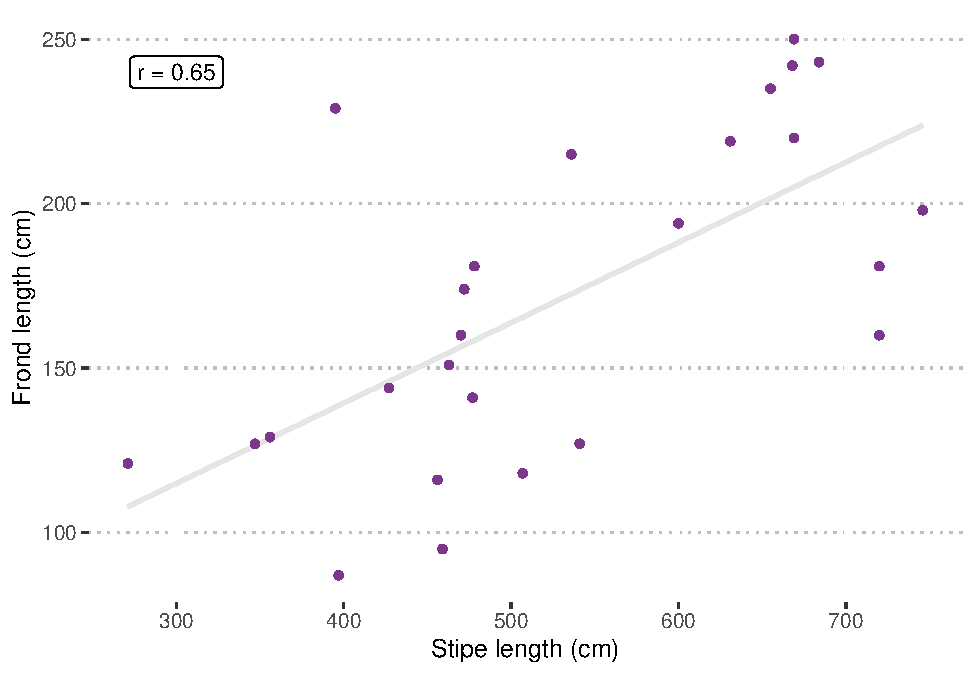
\includegraphics[width=0.7\linewidth]{09-correlations_files/figure-latex/corr-plot1-1}
\textbackslash{}caption\{Scatterplot showing relationship between
\emph{Ecklonia maxima} stipe length (cm) and frond length (cm). The
correlation coefficient (Pearson r) is shown in the top left corner.
Note that the grey line running through the middle is a fitted linear
model and is not generating the correlation value. Rather it is included
to help visually demonstrate the strength of the
relationship.\}\label{fig:corr-plot1} \textbackslash{}end\{figure\}

Just by eye-balling this scatterplot it should be clear that these data
tend to increase at a roughly similar rate. Our Pearson r value is an
indication of what that is.

\hypertarget{multiple-panel-visual}{%
\section{Multiple panel visual}\label{multiple-panel-visual}}

But why stop at one panel? It is relatively straightforward to quickly
plot correlation results for all of our variables in one go. In order to
show which variables correlate most with which other variables all at
once, without creating chaos, we will create what is known as a heat
map. This visualisation uses a range of colours, usually blue to red, to
demonstrate where more of something is. In this case, we use it to show
where more correlation is occurring between morphometric properties of
the kelp \emph{Ecklonia maxima}.

\begin{Shaded}
\begin{Highlighting}[]
\KeywordTok{corrplot}\NormalTok{(ecklonia_pearson, }\DataTypeTok{method =} \StringTok{"circle"}\NormalTok{)}
\end{Highlighting}
\end{Shaded}

\begin{figure}
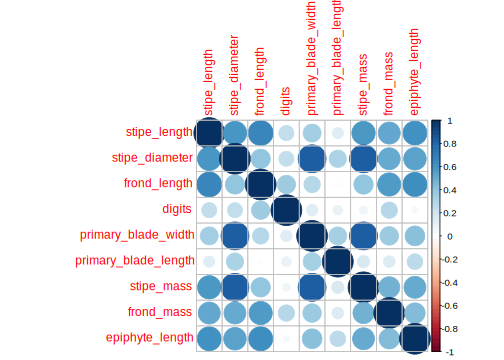
\includegraphics[width=0.7\linewidth]{09-correlations_files/figure-latex/corr-plot2-1} \caption{Correlation plot showing the strength of all correlations between all variables as a scale from red (negative) to blue (positive).}\label{fig:corr-plot2}
\end{figure}

\begin{quote}
\textbf{Task:} What does the series of dark blue circles through the
middle of this plot mean?

\textless{} \textbf{Task:} Which morphometric properties correlate
best/worst?
\end{quote}

Slightly more involved, but much more useful, is the generation of a
heat map using \textbf{\texttt{ggplot2}}.

\hypertarget{exercises-5}{%
\section{Exercises}\label{exercises-5}}

\hypertarget{exercise-1-5}{%
\subsection{Exercise 1}\label{exercise-1-5}}

Produce a heat map using \textbf{\texttt{ggplot2}}.

\hypertarget{confidence-intervals}{%
\chapter{Confidence intervals}\label{confidence-intervals}}

A confidence interval (CI) tells us within what range we may be certain
to find the true mean from which any sample has been taken. To calculate
a confidence interval requires three things:

\begin{Shaded}
\begin{Highlighting}[]
\CommentTok{# First we set the sample mean}
\NormalTok{sample_mean <-}\StringTok{ }\DecValTok{10}

\CommentTok{# Then the sample standard deviation}
\NormalTok{sample_sd <-}\StringTok{ }\DecValTok{2}

\CommentTok{# Then the number of samples}
\NormalTok{sample_n <-}\StringTok{ }\DecValTok{20}
\end{Highlighting}
\end{Shaded}

Once we know these things we must then use the following formula to
calculate th CI:

\begin{Shaded}
\begin{Highlighting}[]
\NormalTok{error <-}\StringTok{ }\KeywordTok{qnorm}\NormalTok{(}\FloatTok{0.975}\NormalTok{)}\OperatorTok{*}\NormalTok{sample_sd}\OperatorTok{/}\KeywordTok{sqrt}\NormalTok{(sample_n)}
\end{Highlighting}
\end{Shaded}

With the CI known, we then substract/add it from the sample mean in
order to find the upper and lower limits:

\begin{Shaded}
\begin{Highlighting}[]
\NormalTok{lower <-}\StringTok{ }\NormalTok{sample_mean}\OperatorTok{-}\NormalTok{error}
\NormalTok{upper <-}\StringTok{ }\NormalTok{sample_mean}\OperatorTok{+}\NormalTok{error}
\NormalTok{lower}
\end{Highlighting}
\end{Shaded}

\begin{verbatim}
R> [1] 9.123477
\end{verbatim}

\begin{Shaded}
\begin{Highlighting}[]
\NormalTok{upper}
\end{Highlighting}
\end{Shaded}

\begin{verbatim}
R> [1] 10.87652
\end{verbatim}

\hypertarget{testing-assumptions-or-how-i-learned-to-stop-worrying-and-transform-the-data}{%
\chapter{Testing assumptions or: How I learned to stop worrying and
transform the
data}\label{testing-assumptions-or-how-i-learned-to-stop-worrying-and-transform-the-data}}

In this chapter we will learn how to test for the two most common
assumptions we will make in the biological sciences.

Our tests for these two assumptions fail often with real data.
Therefore, we must often identify the way in which our data are
distributed so we may better decide how to transform them in an attempt
to coerce them into a format that will pass the assumptions.

Before we begin, let's go ahead and activate our packages and load our
data.

\begin{Shaded}
\begin{Highlighting}[]
\KeywordTok{library}\NormalTok{(tidyverse)}
\NormalTok{chicks <-}\StringTok{ }\KeywordTok{as_tibble}\NormalTok{(ChickWeight)}
\end{Highlighting}
\end{Shaded}

\hypertarget{the-two-main-assumptions}{%
\section{The two main assumptions}\label{the-two-main-assumptions}}

\hypertarget{normality-1}{%
\subsection{Normality}\label{normality-1}}

The quickest method of testing the normality of a variable is with the
Shapiro-Wilk normality test. This will return two values, a W score and
a \emph{p}-value. FOr the purposes of this course we may safely ignore
the W score and focus on the \emph{p}-value. When \emph{p}
\textgreater{}= 0.05 we may assume that the data are normally
distributed. If \emph{p} \textless{} 0.05 then the data are not normally
distrubted. Let's look at all of the \texttt{chicks} data without
filtering it:

\begin{Shaded}
\begin{Highlighting}[]
\KeywordTok{shapiro.test}\NormalTok{(chicks}\OperatorTok{$}\NormalTok{weight)}
\end{Highlighting}
\end{Shaded}

\begin{verbatim}
R> 
R>  Shapiro-Wilk normality test
R> 
R> data:  chicks$weight
R> W = 0.90866, p-value < 2.2e-16
\end{verbatim}

Are these data normally distributed? How do we know? Now let's filter
the data based on the different diets for only the weights taken on the
last day (21):

\begin{Shaded}
\begin{Highlighting}[]
\NormalTok{chicks }\OperatorTok\StringTok{ }
\StringTok{  }\KeywordTok{filter}\NormalTok{(Time }\OperatorTok{==}\StringTok{ }\DecValTok{21}\NormalTok{) }\OperatorTok\StringTok{ }
\StringTok{  }\KeywordTok{group_by}\NormalTok{(Diet) }\OperatorTok\StringTok{ }
\StringTok{  }\KeywordTok{summarise}\NormalTok{(}\DataTypeTok{norm_wt =} \KeywordTok{as.numeric}\NormalTok{(}\KeywordTok{shapiro.test}\NormalTok{(weight)[}\DecValTok{2}\NormalTok{]))}
\end{Highlighting}
\end{Shaded}

\begin{verbatim}
R> # A tibble: 4 x 2
R>   Diet  norm_wt
R>   <fct>   <dbl>
R> 1 1       0.591
R> 2 2       0.949
R> 3 3       0.895
R> 4 4       0.186
\end{verbatim}

How about now?

\hypertarget{homoscedasticity-1}{%
\subsection{Homoscedasticity}\label{homoscedasticity-1}}

Here we need no fancy test. We must simply calculate the variance of the
variables we want to use and see that they are not more than 3 -- 4
times greater than one another.

\begin{Shaded}
\begin{Highlighting}[]
\NormalTok{chicks }\OperatorTok\StringTok{ }
\StringTok{  }\KeywordTok{filter}\NormalTok{(Time }\OperatorTok{==}\StringTok{ }\DecValTok{21}\NormalTok{) }\OperatorTok\StringTok{ }
\StringTok{  }\KeywordTok{group_by}\NormalTok{(Diet) }\OperatorTok\StringTok{ }
\StringTok{  }\KeywordTok{summarise}\NormalTok{(}\DataTypeTok{var_wt =} \KeywordTok{var}\NormalTok{(weight))}
\end{Highlighting}
\end{Shaded}

\begin{verbatim}
R> # A tibble: 4 x 2
R>   Diet  var_wt
R>   <fct>  <dbl>
R> 1 1      3446.
R> 2 2      6106.
R> 3 3      5130.
R> 4 4      1879.
\end{verbatim}

Well, do these data pass the two main assumptions?

\hypertarget{transforming-data}{%
\section{Transforming data}\label{transforming-data}}

\hypertarget{log-transform}{%
\subsection{Log transform}\label{log-transform}}

\hypertarget{section}{%
\subsection{}\label{section}}

\hypertarget{exercises-6}{%
\section{Exercises}\label{exercises-6}}

\hypertarget{exercise-1-6}{%
\subsection{Exercise 1}\label{exercise-1-6}}

Find one of the days of measurement where the chicken weights do not
pass the assumptions of normality, and another day (not day 21!) in
which they do.

\hypertarget{exercise-2-2}{%
\subsection{Exercise 2}\label{exercise-2-2}}

Transform the data so that they may pass the assumptions.

\hypertarget{linear-mixed-models}{%
\chapter{Linear mixed models}\label{linear-mixed-models}}

In the previous chapter we learned how to test hypotheses based on the
comparions of means between sets of data when we were able to meet our
two base assumptions. These parametric tests are preferred over
non-parametric tests because they are more robust. However, when we
simply aren't able to meet these assumptions we must not despair.
Non-parametric tests are still useful. In this chapter we will learn how
to run non-parametirc tests for two sample and multiple sample datasets.
To start, let's load our libraries and \texttt{chicks} data if we have
not already.

\begin{Shaded}
\begin{Highlighting}[]
\CommentTok{# First activate libraries}
\KeywordTok{library}\NormalTok{(tidyverse)}
\KeywordTok{library}\NormalTok{(ggpubr)}

\CommentTok{# Then load data}
\NormalTok{chicks <-}\StringTok{ }\KeywordTok{as_tibble}\NormalTok{(ChickWeight)}
\end{Highlighting}
\end{Shaded}

With our libraries and data loaded, let's find a day in which at least
one of our assumptions are violated.

\begin{Shaded}
\begin{Highlighting}[]
\CommentTok{# Then check for failing assumptions}
\NormalTok{chicks }\OperatorTok\StringTok{ }
\StringTok{  }\KeywordTok{filter}\NormalTok{(Time }\OperatorTok{==}\StringTok{ }\DecValTok{0}\NormalTok{) }\OperatorTok\StringTok{ }
\StringTok{  }\KeywordTok{group_by}\NormalTok{(Diet) }\OperatorTok\StringTok{ }
\StringTok{  }\KeywordTok{summarise}\NormalTok{(}\DataTypeTok{norm_wt =} \KeywordTok{as.numeric}\NormalTok{(}\KeywordTok{shapiro.test}\NormalTok{(weight)[}\DecValTok{2}\NormalTok{]),}
            \DataTypeTok{var_wt =} \KeywordTok{var}\NormalTok{(weight))}
\end{Highlighting}
\end{Shaded}

\begin{verbatim}
R> # A tibble: 4 x 3
R>   Diet  norm_wt var_wt
R>   <fct>   <dbl>  <dbl>
R> 1 1     0.0138   0.989
R> 2 2     0.138    2.23 
R> 3 3     0.00527  1.07 
R> 4 4     0.0739   1.11
\end{verbatim}

\hypertarget{wilcox-rank-sum-test-1}{%
\section{Wilcox rank sum test}\label{wilcox-rank-sum-test-1}}

The non-parametric version of a t-test is a Wilcox rank sum test. To
perform this test in R we may again use \texttt{compare\_means()} and
specify the test we want:

\begin{Shaded}
\begin{Highlighting}[]
\KeywordTok{compare_means}\NormalTok{(weight }\OperatorTok{~}\StringTok{ }\NormalTok{Diet, }\DataTypeTok{data =} \KeywordTok{filter}\NormalTok{(chicks, Time }\OperatorTok{==}\StringTok{ }\DecValTok{0}\NormalTok{, Diet }\OperatorTok\StringTok{ }\KeywordTok{c}\NormalTok{(}\DecValTok{1}\NormalTok{, }\DecValTok{2}\NormalTok{)), }\DataTypeTok{method =} \StringTok{"wilcox.test"}\NormalTok{)}
\end{Highlighting}
\end{Shaded}

\begin{verbatim}
R> # A tibble: 1 x 8
R>   .y.    group1 group2     p p.adj p.format p.signif method  
R>   <chr>  <chr>  <chr>  <dbl> <dbl> <chr>    <chr>    <chr>   
R> 1 weight 1      2      0.235 0.235 0.23     ns       Wilcoxon
\end{verbatim}

What do our results show?

\hypertarget{kruskall-wallis-rank-sum-test-1}{%
\section{Kruskall-Wallis rank sum
test}\label{kruskall-wallis-rank-sum-test-1}}

\hypertarget{single-factor-2}{%
\subsection{Single factor}\label{single-factor-2}}

The non-parametric version of an ANOVA is a Kruskall-Wallis rank sum
test. As you may have by now surmised, this may be done with
\texttt{compare\_means()} as seen below:

\begin{Shaded}
\begin{Highlighting}[]
\KeywordTok{compare_means}\NormalTok{(weight }\OperatorTok{~}\StringTok{ }\NormalTok{Diet, }\DataTypeTok{data =} \KeywordTok{filter}\NormalTok{(chicks, Time }\OperatorTok{==}\StringTok{ }\DecValTok{0}\NormalTok{), }\DataTypeTok{method =} \StringTok{"kruskal.test"}\NormalTok{)}
\end{Highlighting}
\end{Shaded}

\begin{verbatim}
R> # A tibble: 1 x 6
R>   .y.        p p.adj p.format p.signif method        
R>   <chr>  <dbl> <dbl> <chr>    <chr>    <chr>         
R> 1 weight 0.475 0.475 0.48     ns       Kruskal-Wallis
\end{verbatim}

As with the ANOVA, this first step with the Kruskall-Wallis test is not
the last. We must again run a post-hoc test on our results. This time we
will need to use \texttt{pgirmess::kruskalmc()}, which means we will
need to load a new library.

\begin{Shaded}
\begin{Highlighting}[]
\KeywordTok{library}\NormalTok{(pgirmess)}

\KeywordTok{kruskalmc}\NormalTok{(weight }\OperatorTok{~}\StringTok{ }\NormalTok{Diet, }\DataTypeTok{data =} \KeywordTok{filter}\NormalTok{(chicks, Time }\OperatorTok{==}\StringTok{ }\DecValTok{0}\NormalTok{))}
\end{Highlighting}
\end{Shaded}

\begin{verbatim}
R> Multiple comparison test after Kruskal-Wallis 
R> p.value: 0.05 
R> Comparisons
R>     obs.dif critical.dif difference
R> 1-2    6.95     14.89506      FALSE
R> 1-3    6.90     14.89506      FALSE
R> 1-4    4.15     14.89506      FALSE
R> 2-3    0.05     17.19933      FALSE
R> 2-4    2.80     17.19933      FALSE
R> 3-4    2.75     17.19933      FALSE
\end{verbatim}

Let's consult the help file for \texttt{kruskalmc()} to understand what
this print-out means.

\hypertarget{multiple-factors-2}{%
\subsection{Multiple factors}\label{multiple-factors-2}}

The water becomes murky quickly when one wants to perform mutliple
factor non-parametric comparison of means tests. TO that end, we will
not cover the few existing methods here. Rather, one should avoid the
necessity for these types of tests when designing an experiment.

\hypertarget{generalised-linear-models}{%
\section{Generalised linear models}\label{generalised-linear-models}}

\hypertarget{sign-test}{%
\subsection{Sign Test}\label{sign-test}}

\hypertarget{wilcoxon-signed-rank-test}{%
\subsection{Wilcoxon Signed-Rank Test}\label{wilcoxon-signed-rank-test}}

\hypertarget{mann-whitney-wilcoxon-test}{%
\subsection{Mann-Whitney-Wilcoxon
Test}\label{mann-whitney-wilcoxon-test}}

\hypertarget{kruskal-wallis-test}{%
\subsection{Kruskal-Wallis Test}\label{kruskal-wallis-test}}

\hypertarget{generalised-linear-models-glm}{%
\subsection{Generalised linear models
(GLM)}\label{generalised-linear-models-glm}}

\hypertarget{exercises-7}{%
\section{Exercises}\label{exercises-7}}

\hypertarget{exercise-1-7}{%
\section{Exercise 1}\label{exercise-1-7}}

Write out the hypotheses that we tested for in this chapter and answer
them based on the results we produced in class.

\hypertarget{chi-squared}{%
\chapter{Chi-squared}\label{chi-squared}}

A chi-squared test is used when one wants to see if there is a
realtionship between count data of two or more factors.

\begin{Shaded}
\begin{Highlighting}[]
\NormalTok{x <-}\StringTok{ }\KeywordTok{c}\NormalTok{(}\DataTypeTok{A =} \DecValTok{20}\NormalTok{, }\DataTypeTok{B =} \DecValTok{15}\NormalTok{, }\DataTypeTok{C =} \DecValTok{25}\NormalTok{)}
\KeywordTok{chisq.test}\NormalTok{(x)}
\end{Highlighting}
\end{Shaded}

\begin{verbatim}
R> 
R>  Chi-squared test for given probabilities
R> 
R> data:  x
R> X-squared = 2.5, df = 2, p-value = 0.2865
\end{verbatim}

\bibliography{LaTeX/bibliography.bib,LaTeX/packages.bib}


\end{document}
